% http://www.idsc.ethz.ch/education/theses-semester-projects.html
% IDSC LaTeX Thesis Template
% 
% Author(s):	Eric Müller
% 				Institute for Dynamic Systems and Control
% 				Swiss Federal Institute of Technology (ETH) Zurich
% 
% Created:		2004/04/02  (Eric Mueller)
% 
% Notes: Has been tested on Windows 7 + MikTeX + TeXnicCenter
%
% Revisions: 	2009/05/29  (Soren Ebbesen)
% 				    2011/03/22	(Soren Ebbesen)
%             2013/03/08	(Soren Ebbesen)
%             2014/03/13	(Soren Ebbesen)
% ______________________________________________________________________________

% !TEX root = C:\Users\victo\Documents\FME\Q3 - TFM\master-thesis\Thesis.tex

\documentclass[10pt,twoside,a4paper,fleqn]{report}

\usepackage[english,mt]{ethidsc} % Special IDSC styles and commands      	
								 % {german}/english: language of headings, etc.
								 % {st}/bt/mt: {semester}/bachelor/master thesis


								 
							
% Page header (don't change)____________________________________________________
\setlength{\parindent}{0em}                 % Disable parindent
\rhead[\nouppercase{\rightmark}]{\thepage}  % Special headings
\lhead[\thepage]{\nouppercase{\leftmark}}   % Special headings
\cfoot{}                                    % Special headings


% Title page (please fill in)___________________________________________________
\title{Improved robustness of deep learning models through posterior
agreement-based model selection}


\studentA{Victor Jimenez Rodriguez}
\ethidA{97-906-739}
\semesterA{5}
\emailA{vjimenez@student.ethz.ch}

%\studentB{Second Student}
%\ethidB{12-345-678}
%\semesterB{9}
%\emailB{second@student.ethz.ch}

\supervision{Dr. Joao Borges de Sa Carvalho, Dr. Alessandro Torcinovich \\ Prof. Dr. Joachim M. Buhmann}
\date{September 2024}

\identification{IDSC-XX-YY-ZZ} 		% Project identifier

\infopage
\declaration

% Begin document________________________________________________________________
\begin{document}

\maketitle 							% Create title page


% Preamble______________________________________________________________________

\pagenumbering{roman} 				% Begin roman page numbering (i,ii,...)

%---------------------------------------------------------------------------
% Preface

\chapter*{Preface}

The work presented in this thesis was performed at the Information and Science Engineering Group at Institute for Machine Learning (ETH Zurich), during the period October 2023 - September 2024, under
the supervision of Prof. Dr. Joachim M. Buhmann. The thesis was co-supervised at Universitat Politecnica de Catalunya by Prof. Dr. Alexandre Parera i Lluna.

 \cleardoublepage

%---------------------------------------------------------------------------
% Table of contents

 \setcounter{tocdepth}{2}
 \tableofcontents

 \cleardoublepage

%---------------------------------------------------------------------------
% Abstract

\chapter*{Abstract}
 \addcontentsline{toc}{chapter}{Abstract}

 Posterior Agreement (PA) has been proposed as a theoretically-grounded alternative for model
 robustness assessment in covariate shift settings. In this work, we provide further evidence in favor of
 this hypothesis and we explore the use of PA as a model selection criterion for deep learning models in supervised 
 classification tasks. \\
 
 Starting from the theoretical principles leading to PA, we derive a computationally-efficient approximation to its value in 
 discrete hypothesis set problems, and we show that it is a valid alternative to cross-validation in the presence of distribution shifts. Additionally, we follow some threads from the original hypothesis and we extend the use of PA to some other specific settings 
 in which a domain shift can be defined, such as subpopulation (unbalanced) settings, mislabelled datasets and data augmentation strategies.

 \cleardoublepage

%---------------------------------------------------------------------------
% Symbols

\chapter*{Notation}\label{chap:symbole}
 \addcontentsline{toc}{chapter}{Notation}

\section*{Symbols}
\begin{tabbing}
 \hspace*{1.6cm} \= \hspace*{8cm} \= \kill
 $\mathrm{EHC}$ \> Conditional equation \> [$-$] \\[0.5ex]
 $e$ \> Willans coefficient \> [$-$] \\[0.5ex]
 $F,G$ \> Parts of the system equation \> [\unitfrac[]{K}{s}]
\end{tabbing}

\section*{Indicies}
\begin{tabbing}
 \hspace*{1.6cm}  \= \kill
 a \> Ambient \\[0.5ex]
 air \> Air
\end{tabbing}

\section*{Acronyms and Abbreviations}
\begin{tabbing}
 \hspace*{1.6cm}  \= \kill
 NEDC \> New European Driving Cycle \\[0.5ex]
 ETH \> Eidgen\"{o}ssische Technische Hochschule
\end{tabbing}

 \cleardoublepage

%---------------------------------------------------------------------------


% Chapters______________________________________________________________________

\pagestyle{fancy}               	% Fancy headings
\pagenumbering{arabic}				% Begin arabic page numbering (1,2,...)

\chapter{Introduction}\label{sec:introduction}

This chapter aims to set the stage for the detailed analysis and discussion that will follow by 
providing a general overview of the problem of model robustness in 
machine learning and the current approaches to address it.

\section{The robustness challenge}\label{sec:motivation}

The field of machine learning revolves around the ambition of having computers
perform certain tasks without being programmed with task-specific instructions,
but instead by training them to find patterns in a data sample from which these 
instructions can be inferred. During training, algorithms learn from data and
experience to incrementally improve their task performance. In the process, a set
of assumptions are implicitly adopted about the statistical model generating the data 
and its connection with the desired task outcome. These assumptions constitute an 
inductive bias, and both architectures and training procedures are designed to
learn optimal biases that generalize to unseen data samples and thus lead to robust
implementations of the task at hand
\cite{p.murphyProbabilisticMachineLearning2022,m.bishopPatternRecognitionMachine2006}.
This project will focus on the assessment of the robustness of deep learning models 
performing image classification tasks.\\ 

In a broad sense, robustness can be defined as the ability of a machine learning 
model to maintain its predictive power on observations that present 
some kind of transformation or variation 
with respect to the ones used for its training
\cite{quinonero-candelaDatasetShiftMachine2009}.
Overall, three sources of variability are relevant in the context
of image classification, namely sampling randomness, adversarial
perturbations and distribution shift, which are illustrated in Figure \ref{fig:cows} 
\cite{buhmannPosteriorAgreementModel2022}.\\

Out of these, only sampling randomness is commonly accounted for by 
standard model validation techniques, in the sense that model selection 
and benchmarking are conducted using randomized subsets of unseen observations. 
In this way, the most generalizable features, and in turn the most generalizable 
models, are naturally selected. As it will be outlined in this chapter, 
this approach presents fundamental limitations
that are rooted in the very nature of deep learning models and
the data from which they learn. \\

First, the operative principles of neural networks make them vulnerable
to small perturbations in the input space, which are
often filtered out in human perception, that can lead to high-confidence
incorrect predictions \cite{szegedyIntriguingPropertiesNeural2014}.
This issue is commonly known as adversarial
vulnerability, and an ongoing arms race incentivizes the design 
of new ways of perturbing models and new ways of defending them
against such attacks. Strategies 
that foster robustness to adversarial attacks are possible, but
come at a price of hindering conventional generalization to 
sampling randomness in the original data \cite{tsiprasRobustnessMayBe2019}. \\

Second, the nature of the data used for training and selecting
models is known to influence heavily the features that the model 
will learn to be the most predictive. The lack of representativity of 
certain aspects of the data or the presence of spurious 
correlations can lead to models that generalize well to sampling 
randomness within the same experiment but that fail to do so when those 
accidental relationships are not present. This is known as an
out-of-distribution setting, given that samples in which the model is tested
are not drawn from the same probability distribution that generated
training samples \cite{quinonero-candelaDatasetShiftMachine2009}. \\

At the core of the robustness challenge lies the poor
understanding of how models construct their inductive bias and the nature
of the transformations between the space of weights and the space of 
functions that they are able to represent \cite{jimenezInductiveBiasDeep}. 
Features learned by the optimal standard classifier can be completely 
different from those learned by a robust classifier, regardless 
of the amount of data provided, which results in a fundamental limitation for task 
performance in robust models \cite{tsiprasRobustnessMayBe2019,zhangTheoreticallyPrincipledTradeoff2019}.
Besides, the feature space that deep learning models navigate is fundamentally 
different than that in which humans implicitly rely on, and we 
should therefore not expect models to be invariant to the 
same features humans are instinctively invariant to \cite{ilyasAdversarialExamplesAre2019}. \\

\begin{figure}
    \centering
    \begin{subfigure}[b]{0.22\textwidth}
        \centering
        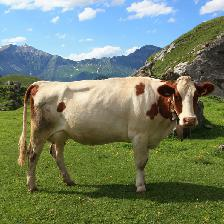
\includegraphics[width=\textwidth]{img/introduction/cow_original.jpg}
        \caption{Original}
    \end{subfigure}
    \hfill
    \begin{subfigure}[b]{0.22\textwidth}
        \centering
        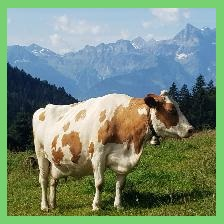
\includegraphics[width=\textwidth]{img/introduction/cow_noise.jpg}
        \caption{Sampling}
    \end{subfigure}
    \hfill
    \begin{subfigure}[b]{0.22\textwidth}
        \centering
        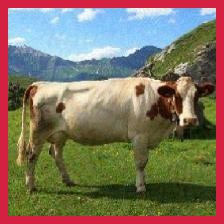
\includegraphics[width=\textwidth]{img/introduction/cow_fgsm.jpg}
        \caption{Adversarial}
    \end{subfigure}
    \hfill
    \begin{subfigure}[b]{0.22\textwidth}
        \centering
        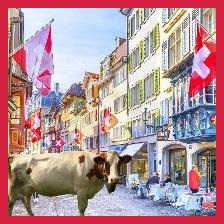
\includegraphics[width=\textwidth]{img/introduction/cow_ood.jpg}
        \caption{Distribution}
    \end{subfigure}
       \caption{Illustrative example of the three expected sources of variability. 
       A pre-trained MobileNetV2 model is shown to be vulnerable to adversarial perturbations 
       as the one represented in (c), and also to distribution shifts 
       as the one illustrated in (d), possibly because its inductive bias is influenced
       by the spurious correlation between cows and rural landscapes.}
       \label{fig:cows}
\end{figure}

This thesis will encompass all these phenomena under the same theoretical
framework, and devise a common approach to the measurement of
the shift entailed by both adversarial and distribution
variability sources. Robustness will be characterized from the space of
outcomes of the model, by means of a (posterior) probability 
distribution that will rank models and algorithms according to the
agreement in their predictions when facing different realizations of the same experiment.

\subsection{Adversarial setting}

As it was previously mentioned, certain perturbations on
original test images, which can be almost imperceptible
to the human eye, can lead to highly-confident but
incorrect predictions by deep neural networks, even when their
standard performance metrics are high.
Adversarial examples have been shown to transfer
across architectures and training procedures, and
even across subsets of data,
often yielding the same incorrect prediction in
all of these cases \cite{szegedyIntriguingPropertiesNeural2014}. \\

These intriguing phenomena were initially hypothesized to arise 
from a lack of smoothness over the input space, a property
commonly assumed in other learners, that derives from the
non-linear nature of deep learning architectures. Nevertheless,
extensive research on the field has elucidated that the root
cause is instead the linearity of its learning units, which makes them
vulnerable in certain directions of high-dimensional
spaces where small
effects can add up to significally change the outcome
\cite{goodfellowExplainingHarnessingAdversarial2015}. \\

Building on this intuition, numerous attacks have been proposed to evaluate the 
robustness of models against adversarial samples. A common strategy for inducing model 
failure involves identifying vulnerable directions in the feature space and adjusting 
perturbations to produce the desired misleading effect. Adversarial examples 
generated through these attacks can then be used to train robust models through 
regularization, thereby promoting generalization to the features present in 
worst-case examples and thus selecting models that are insensitivized
to them
\cite{baiRecentAdvancesAdversarial2021}.\\

Nevertheless, adversarial learning entails decision boundaries 
that are more complex than the ones derived via standard training
(see Figure \ref{fig:adversarial_complexity}), 
intuitively demanding more data and more complex 
architectures, at the risk of
overfitting to adversarial examples themselves
\cite{schmidtAdversariallyRobustGeneralization2018}. 
These limitations express a fundamental trade-off 
that arises from the intrinsic 
disparity between robust and non-robust features
\cite{tsiprasRobustnessMayBe2019, zhangTheoreticallyPrincipledTradeoff2019}. \\

\begin{figure}
    \centering
    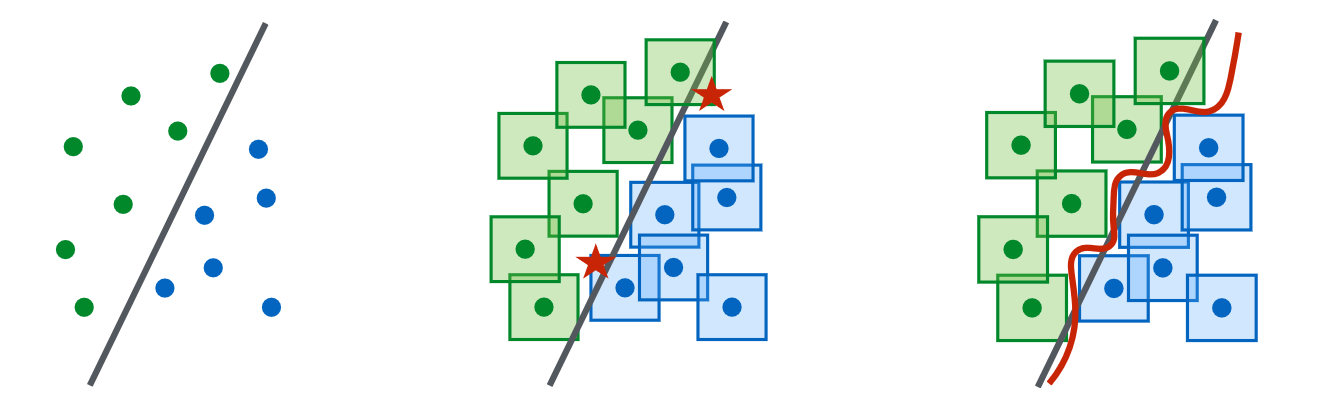
\includegraphics[width=0.65\textwidth]{img/introduction/adversarial_complexity.png}
    \caption{
    A conceptual illustration of standard vs. adversarial 
    decision boundaries. (\textbf{left}) A set of linearly-separable points. 
    (\textbf{middle}) Decision boundary learned via standard training.
    (\textbf{right}) Decision boundary learned via adversarial training.
    Both methods achieve zero training error, but only the robust model
    is able to generalize to $\ell_\infty$ perturbations.
    \cite{madryDeepLearningModels2019}
    }
    \label{fig:adversarial_complexity}
\end{figure}

Features selected via standard training
are the most predictive towards generalizing
to sampling randomness within the same dataset, but they do
not necessarily represent the features implicitly selected 
by humans and are not invariant to a human-based notion 
of similarity. Instead, features selected via adversarial training 
have been shown to better model this
invariance, and thus align much better with 
human perception, as seen in Figure \ref{fig:adversarial_loss}
\cite{ilyasAdversarialExamplesAre2019}. Furthermore, adversarial perturbations of robust 
models display salient characteristics;
that is, features that are perceived to belong to the
class they are misclassified to, as illustrated in Figure \ref{fig:salient_characteristics}
\cite{tsiprasRobustnessMayBe2019}. \\

\begin{figure}[H]
    \centering
    \begin{subfigure}[b]{0.28\textwidth}
        \centering
        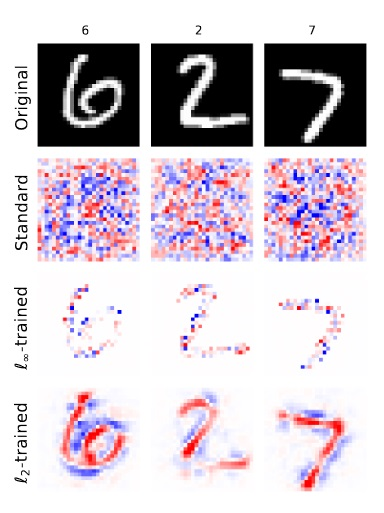
\includegraphics[width=\textwidth]{img/introduction/adversarial_loss_1.jpg}
        \caption{MNIST}
    \end{subfigure}
    \hspace{1cm}
    \begin{subfigure}[b]{0.28\textwidth}
        \centering
        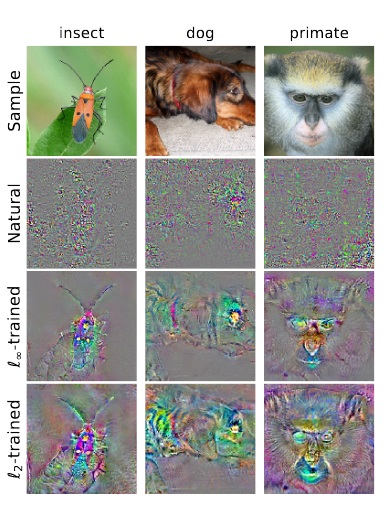
\includegraphics[width=\textwidth]{img/introduction/adversarial_loss_2.jpg}
        \caption{Restricted ImageNet}
    \end{subfigure}
       \caption{Scaled loss gradient with respect to input images.
       Input pixels yielding the highest predictive power are aligned 
       with perceptually relavant features for the case of adversarial
       models, while appearing completely random in the case of 
       standard models.
       \cite{tsiprasRobustnessMayBe2019}}
       \label{fig:adversarial_loss}
\end{figure}


\begin{figure}[H]
    \centering
    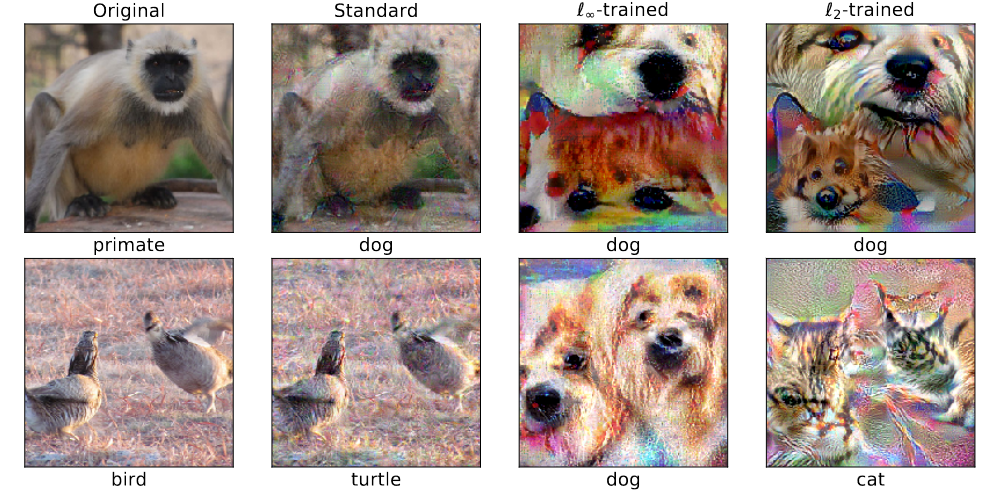
\includegraphics[width=0.45\textwidth]{img/introduction/adversarial_salient.png}
    \caption{Adversarial examples for standard and adversarially-trained models.
    Perturbed images produced for robust models 
    effectively capture salient data characteristics.
    % and appear similar to examples of a different class. 
    \cite{tsiprasRobustnessMayBe2019}}
    \label{fig:salient_characteristics}
\end{figure}

Overall, these and other findings suggest that robustness in the adversarial setting
is a fundamental property of the data features that are represented by models, 
rather than of the models themselves, and the phenomenon of transferability can be
explained in these terms. Training strategies that manage to navigate the 
robustness-generalization trade-off will be the ones yielding 
the best results, provided that the data distribution
is representative of the true underlying features. 

\subsection{Out-of-distribution setting}\label{sec:intro_ood}

Most learning algorithms work under the fundamental assumption that
a causal relationship exists between input and output spaces. The target function to 
learn represents that causality and must therefore remain 
invariant regardless of the available data, which implies that 
suitable approximations of this 
function can be obtained as long as data samples are independent 
and identically distributed in the input space
\cite{muandetDomainGeneralizationInvariant2013,quinonero-candelaDatasetShiftMachine2009}. 
Nevertheless, this is not always
the case, as often real-world data does not match the same statistical
patterns of the data used for training. Ultimately, this phenomenon induces a
distribution shift that leads to poor generalization performance
\cite{zhouDomainGeneralizationSurvey2022,wangGeneralizingUnseenDomains2022,liuOutOfDistributionGeneralizationSurvey2023}. \\

\begin{figure}[h]
    \centering
    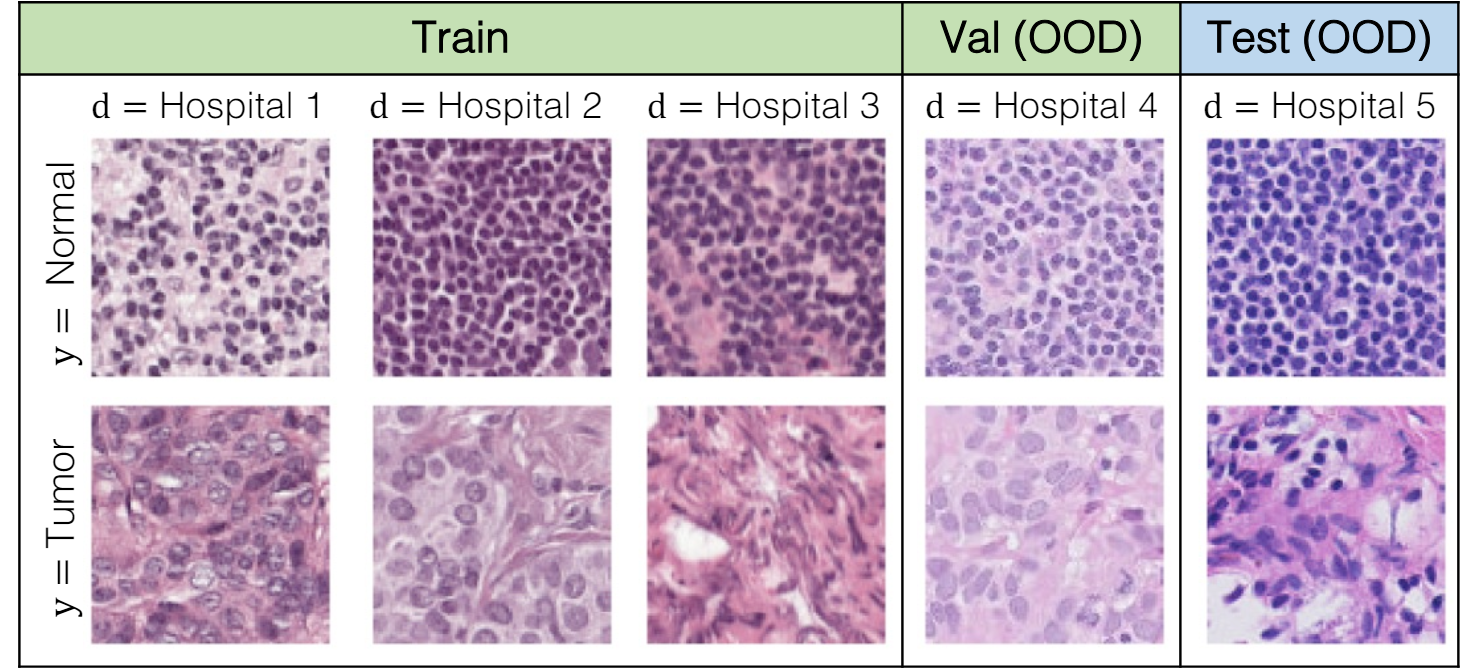
\includegraphics[width=0.5\textwidth]{img/introduction/camelyon17.png}
    \caption{The \texttt{camelyon17} (WILDS) dataset comprises images of stained 
    lymph node tissue patches sampled from different hospitals.
    \cite{kohWILDSBenchmarkIntheWild2021}
    }
    \label{fig:camelyon17}
\end{figure}

A distribution shift can arise for various reasons, namely the 
unfeasibility of collecting diverse enough data, the changing or time-dependent
nature of the data, or the implicit bias
introduced during the data collection process. This last case
is particularly relevant, as it can serve as a generalization of all
the previous cases and raise epistemological questions
about the learning framework itself. For instance, 
Figure \ref{fig:dataset_bias} refers to a cross-generalization analysis in which popular
machine learning datasets were shown to be biased towards
specific representation of features. Considering the fact that all
data is sampled from the same source (i.e. Internet), 
numerous human-induced biases are shown to determine the 
nature of representations, the most significant of all being 
negative bias, which arises when the negative subset\footnote{
    When certain observations in a dataset are labelled as belonging 
    to a specific class, the remaining observations are implicitly
    assigned to not belong to that class, and therefore define a
    negative set in the model's feature space.
}
of the dataset is not representative of the input subspace 
excluding that  particular class and results in a model that performs 
significantly worse in other datasets, even when trained with 
the same observations of that class.\\

\begin{figure}[H]
    \centering
    \begin{subfigure}[b]{0.35\textwidth}
        \centering
        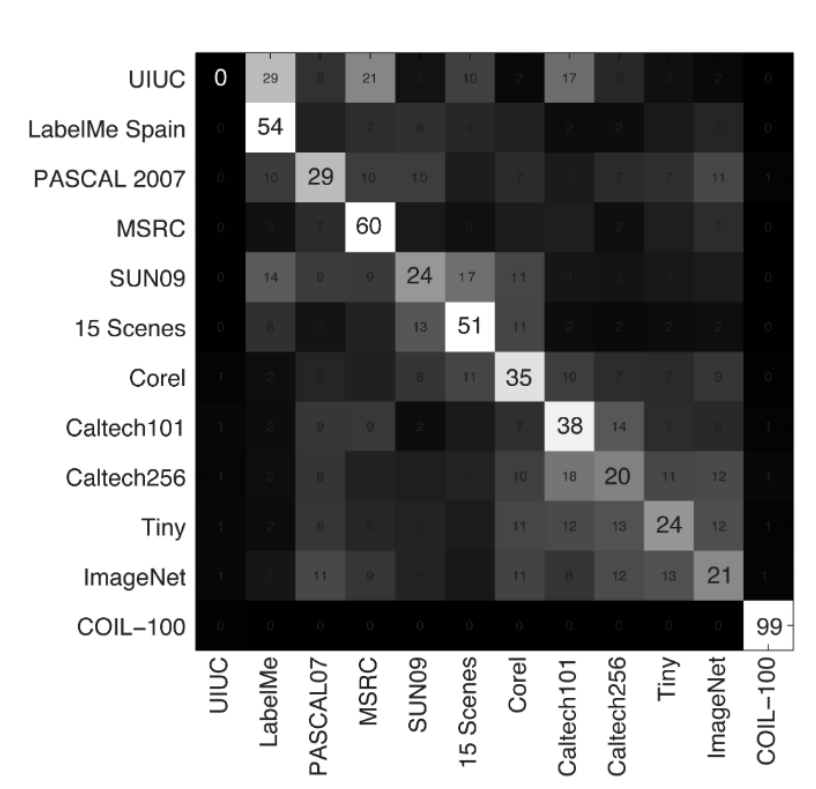
\includegraphics[width=\textwidth]{img/introduction/dataset_bias_confusion.png}
    \end{subfigure}
    \hspace{1cm}
    \begin{subfigure}[b]{0.32\textwidth}
        \centering
        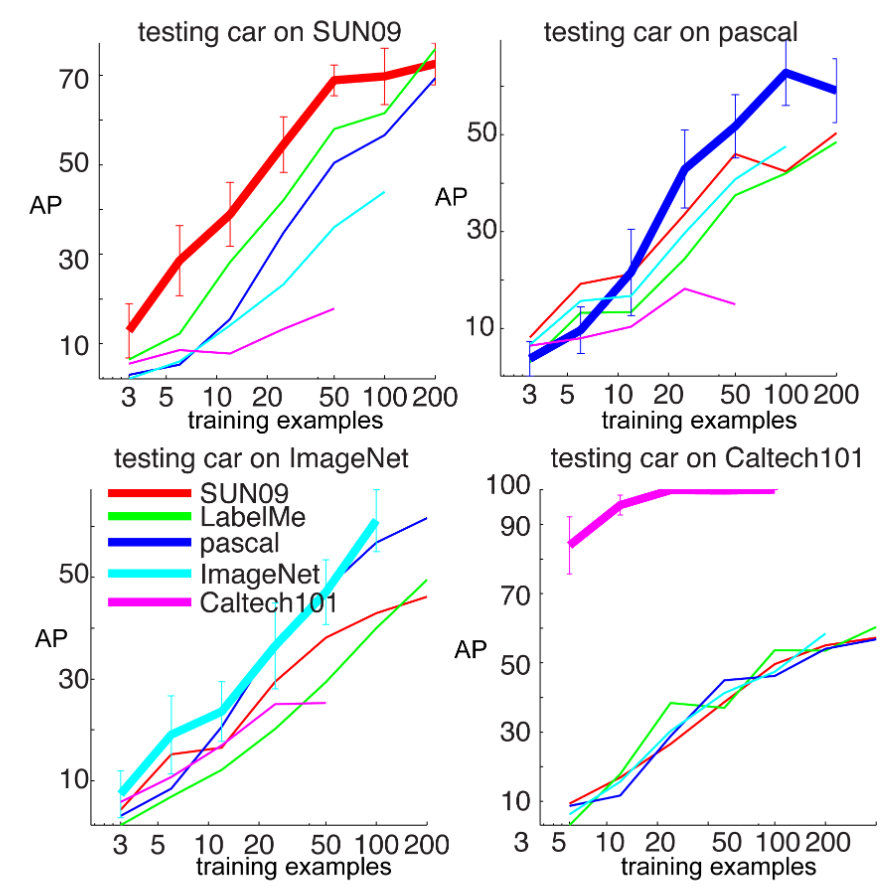
\includegraphics[width=\textwidth]{img/introduction/dataset_bias_cross_generalization.png}
    \end{subfigure}
       \caption{
        \textbf{(left)} Confusion matrix generated in a dataset
        identification task. A clearly pronounced diagonal 
        indicates that each dataset posesses unique traits that
        make it distinguishable from the rest.
        \textbf{(right)} Cross-dataset generalization
        for \texttt{car} detection as function of training data. 
        The vertical gap between lines represents the decrease in performance 
        when training on a different dataset, and the horizontal 
        shift corresponds to the increase in the amount of data needed 
        to reach the same performance.
        \cite{torralbaUnbiasedLookDataset2011}}
       \label{fig:dataset_bias}
\end{figure}

Several approaches can be taken to address this issue, depending
on the nature of the shift and the accessibility of the
causal structure of the data (see Figure 3 and Table 2 in 
\cite{wangGeneralizingUnseenDomains2022}).
Nevertheless, the common goal is to push the model towards
domain-invariant representations that foster robustness in the
face of distribution shifts, sometimes relaxing the causality condition
to an assumption of invariance or stability of the distribution in the output space
\cite{wangGeneralizingUnseenDomains2022,liuOutOfDistributionGeneralizationSurvey2023}. \\

In general, every formulation considers a set of source domains 
encompassing data that is available for the training of the model,
including any validation subsets used for model selection, 
regularization or hyperparameter tuning, and a set of target 
domains encompassing unseen data on which model performance will
be evaluated. Within this framework, a straightforward approach
to improving robustness is to directly sample target domains
and adjust feature representations to be invariant 
between both, which is commonly known as domain adaptation. \\

In this work we will focus instead on domain generalization, which 
refers to the case in which target domains are not accessible 
and feature invariance can be only enforced
from source domains
\cite{blanchardGeneralizingSeveralRelated}. In particular, two strategies will be considered, 
namely domain alignment and data augmentation/generation. \\

On the one hand, domain alignment stems from the target invariance hypothesis, 
and can be formulated as a regularization problem that pushes towards the 
minimization of the dissimilarity of feature  representations originated 
from different source environments. The feature space in which the 
alignment is performed (e.g. a kernel latent space, as Figure \ref{fig:dica} illustrates)
and the similarity metric considered will
determine the peculiarity of the method
\cite{shenWassersteinDistanceGuided2018,liangComprehensiveSurveyTestTime2023}. \\

\begin{figure}[H]
    \centering
    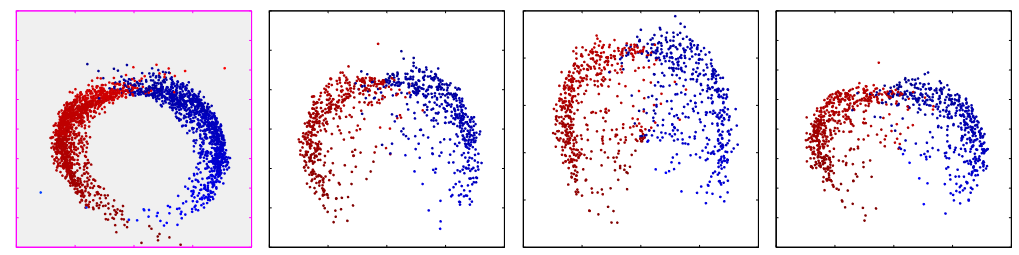
\includegraphics[width=0.65\textwidth]{img/introduction/dica.png}
    \caption{
    Projections of a binary synthetic dataset in the two principal DICA
    dimensions. The shaded box depicts the projection of training 
    data, whereas the unshaded boxes show projections of unseen 
    test datasets. \cite{muandetDomainGeneralizationInvariant2013}
    }
    \label{fig:dica}
\end{figure}

\begin{figure}[H]
    \centering
    \begin{subfigure}[b]{0.2\textwidth}
        \centering
        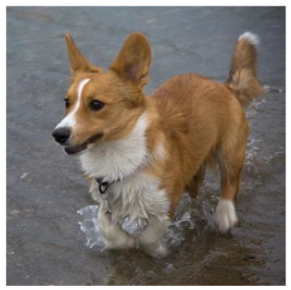
\includegraphics[width=\textwidth]{img/introduction/da_original.png}
        \caption{Original}
    \end{subfigure}
    \hspace{1cm}
    \begin{subfigure}[b]{0.2\textwidth}
        \centering
        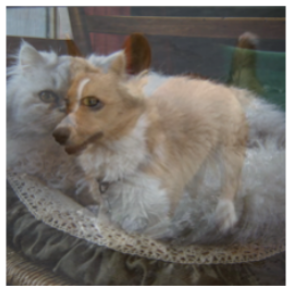
\includegraphics[width=\textwidth]{img/introduction/da_mixup.png}
        \caption{Mixup 
        \cite{zhangMixupEmpiricalRisk2018}
        }
    \end{subfigure}
    \hspace{1cm}
    \begin{subfigure}[b]{0.2\textwidth}
        \centering
        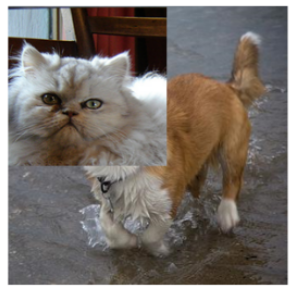
\includegraphics[width=\textwidth]{img/introduction/da_cutmix.png}
        \caption{CutMix
        \cite{yunCutMixRegularizationStrategy2019}
        }
    \end{subfigure}
       \caption{
        Mixup and Cutmix strategies can be used to interpolate
        between different labels and/or domains
        by generating intermediate observations.
        \cite{yunCutMixRegularizationStrategy2019}
        }
       \label{fig:data_augmentation}
\end{figure}

On the other hand, data augmentation/generation strategies 
do not need to assume target invariance and instead 
achieve cross-domain generalization by generating artificial observations that
diversify the original dataset with the hope of capturing 
the underlying causal structure of the data generation process. Augmented observations
can either be randomizations of original observations (e.g. transformations
such as rescaling or rotations) or new samples filling the distribution
gaps between domains (e.g. through interpolation, as illustrated 
in Figure \ref{fig:data_augmentation}). \\

Unlike in the adversarial setting, there is no common way of measuring
the shift in distribution betweeen source domains, and current approaches
are often constrained to specific datasets or training strategies. 
Robustness is instead quantified during (cross-)validation, either by reserving
a subset of each domain, leaving one domain out or
directly accessing target domains if they are available, 
which is known as the oracle approach. This last strategy is often
used to provide an upper bound estimate of model robustness, 
as it usually provides over-confident performance estimates
\cite{zhouDomainGeneralizationSurvey2022}.
Numerous benchmark datasets, some of which will be considered in this work, are the current 
standard for robustness assessment even with
the limitations they present
\cite{kohWILDSBenchmarkIntheWild2021}. 
\\

%Despite extensive research on the field and a wide variety
%of strategies envisionated, robustness to distribution shifts 
%continues to pose a fundamental challenge in machine learning. As
%previously mentioned, this difficulty primarily arises from the 
%violation of the sampling uniformity assumption, which renders 
%conventional learning techniques ineffective, and also from the 
%lack of a universal formal characterization of distribution shifts.
%Existing benchmark datasets, some of which will be considered in this work, are the current 
%standard for robustness assessment even with
%the limitations they present. \\

\section{Related work}

In the adversarial front, early work 
\cite{szegedyIntriguingPropertiesNeural2014}
unveiled the nature of the susceptibility of deep learning 
models to adversarial examples and FGSM 
\cite{goodfellowExplainingHarnessingAdversarial2015}
was introduced as an intuitive
approach for robust regularization. 
Since then, several gradient-based methods have been
proven to enhance adversarial robustness, such as PGD
\cite{madryDeepLearningModels2019}, C\&W 
\cite{carliniEvaluatingRobustnessNeural2017},
FMN
\cite{pintorFastMinimumnormAdversarial2021} and
many others (see 
\cite{liReviewAdversarialAttack2022} for reference). 
All of them ultimately entail a strategy to find
a vulnerable direction and adjust the perturbation 
(e.g. minimum-norm, maximum-confidence, etc.)
based on the location of the decision boundary, either via soft
constraints (i.e. regularization), boundary attacks or gradient
projections
\cite{baiRecentAdvancesAdversarial2021}. \\

In general, the primary distinction among adversarial attacks lies in
their knowledge of the model's architecture and parameters. In that
sense, white-box and black-box
attacks can be distinguished, where the former have full 
access to the model and the latter only 
to the model's predictions. In black-box settings, the loss gradient
is unknown and other strategies such as score-based or
decision-based attacks are used
\cite{liReviewAdversarialAttack2022}. Regarding adversarial training (i.e. defenses), 
robustness can
be achieved by a variety of methods, 
such as ensemble learning,
defensive distillation,
generative adversarial networks
\cite{xiaoGeneratingAdversarialExamples2019, miyatoVirtualAdversarialTraining2018},
diffusion models
\cite{wangBetterDiffusionModels2023,hoDenoisingDiffusionProbabilistic2020}
and adaptive-boundary methods
\cite{cohenCertifiedAdversarialRobustness2019}.
In this project, the Robustbench attack library
\cite{croceRobustBenchStandardizedAdversarial2021a}
will be leveraged to evaluate adversarial robustness 
in the CIFAR10 dataset
\cite{krizhevskyLearningMultipleLayers}. \\

In the domain generalization front, the existing rich taxonomy 
of methods can be classified into two main groups, namely
data manipulation and representation learning 
\cite{wangGeneralizingUnseenDomains2022,zhouDomainGeneralizationSurvey2022,liuOutOfDistributionGeneralizationSurvey2023}.
First, data manipulation strategies involve both augmentation and generation,
as for example image randomization or adversarial augmentation
\cite{yaoImprovingOutofDistributionRobustness2022,zhangMixupEmpiricalRisk2018,yunCutMixRegularizationStrategy2019}.
Second, representation learning strategies are primarily divided 
into domain-invariant methods (e.g. model-based
\cite{arjovskyInvariantRiskMinimization2020},
kernel-based
\cite{muandetDomainGeneralizationInvariant2013,arjovskyWassersteinGAN2017}
or adversarial-based
\cite{peiMultiAdversarialDomainAdaptation}) 
and feature disentanglement methods, which encompass causality-inspired
approaches and general multi-component analysis. Other 
learning strategies include meta-learning,
ensemble learning or self-supervised learning
\cite{liLearningGeneralizeMetaLearning2018,wangMetaFineTuningNeural2020}. \\

Regarding robustness characterization, a wide range of metrics
have been conceived (see
\cite{guoComprehensiveEvaluationFramework2023}), but
accuracy-based criteria are still the most common. As an alternative, 
some  theoretically-grounded approaches have been proposed, such
as CLEVER \cite{wengEvaluatingRobustnessNeural2018}, ACTS 
\cite{wangGeometricalApproachEvaluate2023}
or
PA
\cite{buhmannPosteriorAgreementModel2022}, 
which is the one explored in this work. 
In general, robustness is often reported and compared using 
robustness benchmark datasets. Some of the most relevant
for image classification tasks are 
MNIST 
\cite{lecun1998mnist}
(and its multiple variations, such as DiagVib-6
\cite{euligDiagViB6DiagnosticBenchmark2021}),
PACS
\cite{yuPACSDatasetPhysical2022},
VLCS
\cite{khoslaUndoingDamageDataset2012}
or WILDS
\cite{kohWILDSBenchmarkIntheWild2021}.

\section{Objectives}

The main goal of this project is to assess
the suitability of the posterior agreement framework in the 
context of deep learning model robustness for image 
classification tasks. For that, an operative version of posterior
agreement for finite, discrete hypothesis classes must be derived and
efficiently implemented, so that it can be used as a metric to evaluate 
and select models based on the robustness of their response to different 
sources and levels of randomness. The results obtained should be compared
with the current state-of-the-art in robustness evaluation, namely
Robustbench
\cite{croceRobustBenchStandardizedAdversarial2021a}
and WILDS 
\cite{kohWILDSBenchmarkIntheWild2021}
benckmarks in the adversarial and
out-of-distribution settings, respectively, and an overall
analysis of the use of the metric as an early-stopping 
criterion should be provided.\\

In order to conduct a comprehensive assessment, a series of steps should be undertaken in a 
deductive manner, so that evidence is provided starting from first principles and culminating
with performance evaluations on benchmark datasets. To begin with, the content of this work should
be self-contained, and for that a formal statement of the learning problem should be given. Both 
learning algorithms and classification models should be defined, including the nuances of their
parametrization via deep neural networks. \\

Next, the robustness challenge should be formulated within the framework of probability theory,
providing a rigorous mathematical foundation for understanding the principal sources of randomness that
are relevant in the context of this work. The generalization capabilities to specific sources of randomness
will determine the robustness score of a model, which for PA is conceived as a 
measure of the stability of the probabilistic output of the model to the randomness of the data 
sampling process. In this sense, the fundamental generalization-complexity trade-off must be reframed
within the context of information theory by relating complexity to the expected information content
of the data. The estimated informativeness will determine the resolution of the hypothesis space and
thus its stability under perturbations of various kinds. Once an operative PA metric is derived, 
its properties should be investigated and further assessed with artificial data, so that PA can be compared 
with baseline accuracy-based metrics at a fundamental level. \\

Experiments should be performed the adversarial setting first, for being adversarial perturbations
intentionally designed to change the prediction of the model and thus entailing a performance-based notion of
robustness that aligns with accuracy measures. After that, a customized implementation of 
the DiagVib-6 
\cite{euligDiagViB6DiagnosticBenchmark2021} 
syntetic data generation pipeline should be used to evaluate the suitability of PA in the domain
generalization setting. This will allow for a detailed analysis of the model selection capabilities of PA 
under different experimental conditions, especially regarding the source, power and rate of the shift 
entailed by each dataset and the accessibility of target domains for model validation and selection.\\


All in all, both analytical and numerical tools should be used to provide a comprehensive analysis
of the model-selection capabilities of PA and the source of its discriminative power. \\





\cleardoublepage
\chapter{Theoretical Background }\label{sec:theory}

\section{The learning framework}

Statistical learning theory encompasses the mathematical framework used to
study generalization in machine learning. In this formalism, the goal
is to learn a target function $f^*: \mathcal{X} \to \mathcal{Y}$ by means of an approximated
function $f \in \mathcal{F}$ using a finite set of observations. 

\begin{definition}[Supervised dataset]
    Let $\mathcal{X} \subseteq \mathbb{R}^d$ and $\mathcal{Y} \subseteq \mathbb{R}^t$ be
    the input and output spaces, respectively. Let $X$ be the random variable associated
    with the sampling in $\mathcal{X}$, and $\underbar{X} = (X_1, ..., X_N) \overset{\text{iid}}{\sim} X$ be a $N$-sized simple
    random sample of $X$. A supervised dataset $D$ is a realization of $\underbar{X}$ paired with its $f^*$-mapped output values.

    $$
    D = \{(\bm{x}_n, f^*(\bm{x}_n))\}_{n \in [N]}
    $$
\end{definition}

\subsection{Empirical risk minimization}

The quality of the approximation can be measured with the expected risk $\mathcal{R}(f)$

$$
\mathcal{R}(f)=\mathbb{E}_{x \sim X}[\mathcal{L}(f(x),f^\star(x))]
$$

where $\mathcal{L}: \mathcal{Y} \times \mathcal{Y} \to \mathbb{R}$ denotes a loss function. Glivenko-Cantelli theorem allow us to
estimate the expected risk with its empirical (plug-in) equivalent when $N$ is large enough.

\begin{definition}[Empirical risk] Let $D$ and $\mathcal{L}$ be the dataset and loss function of our problem, respectively. The empirical risk of $f \in \mathcal{F}$
    computed on $D$ is defined as

    $$
    \hat{\mathcal{R}}_D(f)=\frac{1}{N}\sum_{n=1}^{N}\mathcal{L}(f(\bm{x}_{n}),f^{\star}(\bm{x}_{n}))
    $$
\end{definition}

Training, therefore, amounts to minimizing the empirical risk over the function class $\mathcal{F}$.

$$
\text{ERM}_D = \hat{f}_D = \min_{f \in \mathcal{F}} \hat{\mathcal{R}}_D(f)
$$

The best learning algorithm will be that minimizing the difference between the 
expected and empirical risks computed on a different realization of the data. 

\begin{definition}[Empirical generalization error] Let $D_{t}$ and $D_v$ be two supervised datasets. Let $\hat{f}^* \in \mathcal{F}$ be the function minimizing the expected risk
    , and let $\hat{f}_{D_t}$ be the function minimizing the empirical expected risk computed on $D_t$. The empirical generalization error of $f_{D_t}$ computed on $D_v$ is defined as

    $$
    \mathcal{E}(D_t, D_v) = \hat{\mathcal{R}}_{D_v}(\hat{f}_{D_t}) = [\hat{\mathcal{R}}_{D_v}(\hat{f}) - \hat{\mathcal{R}}_{D_v}(\hat{f}^*)] + \hat{\mathcal{R}}_{D_v}(\hat{f}^*) = \mathcal{E}_{\text{estimation}}+ \mathcal{E}_{\text{capacity}}
    $$

    where $\mathcal{E}_{\text{capacity}}$ is governed by the ability of the function class $\mathcal{F}$ to represent the target function; i.e. its complexity.
\end{definition}


The definition of complexity depends on the problem, but intuitively measures the cardinality of the
subset of $\mathcal{F}$ that the algorithm is able to represent. A complex or high-capacity algorithm will
be able to represent a larger subset of $\mathcal{F}$ and achieve a low empirical error, but will be also
prone to overfitting to the specific learning realization thus yielding a higher generalization error. 

\subsection{Regularized risk minimization}

As a general principle, the inductive bias of the algorithm (i.e. the set of constraints imposed on $\mathcal{F}$ during learning) should be aligned with
that of our target function. Given that more expressive classes are always preferred by optimization algorithms, the ERM
objective function is usually tweaqued to include a regularization term penalizing complexity.

\begin{definition}[Regularized empirical risk] Let $\Omega: \mathcal{F} \to \mathbb{R}$ be a complexity measure. The regularized empirical risk of a function $f$
    computed on $D$ is defined as

    $$
    \hat{\mathcal{R}}_{\Omega}(f)=\hat{\mathcal{R}}(f) + \lambda \Omega(f)
    $$

    where $\lambda \in \mathbb{R}$ controls the trade-off between empirical risk and generalization error.

\end{definition}

The RRM problem now includes a hyperparameter $\lambda$, that will be selected so that the generalization error is minimized.

\section{Learning with neural networks}

Neural networks are biologically-inspired machine learning models that consist of a set of 
nodes (neurons) organized in layers and connected by weighted edges (synapses). Figure \ref{fig:nn_node} shows the 
data transformation performed by a single node.

\begin{figure}[H]
    \centering
    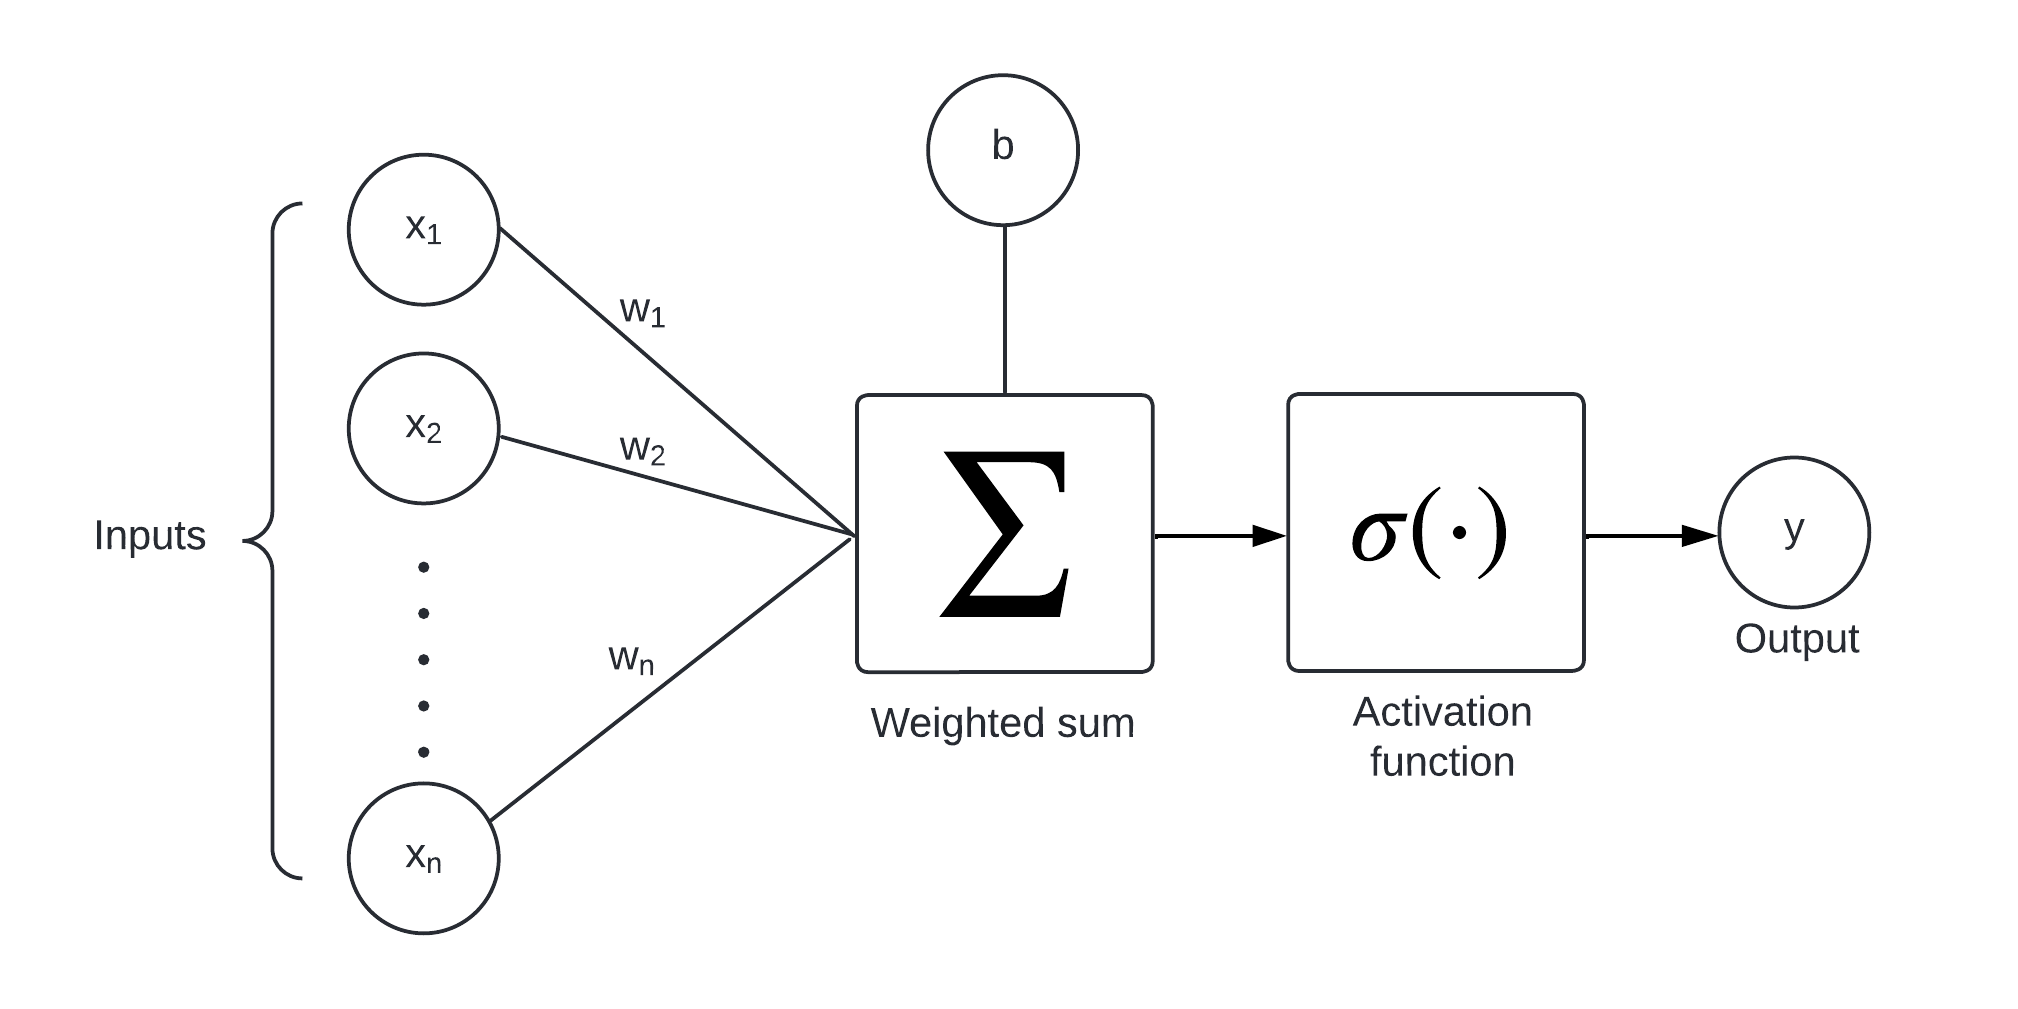
\includegraphics[width=0.4\textwidth]{img/theoretical_background/nn_node.png}
    \caption{The output of a node is computed by applying a non-linear
    activation function $\sigma(\cdot)$ to the weighted sum of its inputs.}
    \label{fig:nn_node}
\end{figure}

Let $\bm{x}_k \in \mathbb{R}^{d_k}$ be the input to the layer $k$, and let $\bm{W} \in \mathbb{R}^{d_k \times d_{k+1}}$ be the $k$-th weight matrix. The output of the layer can be expressed as

$$
\bm{x}_{k+1} = \sigma_k(\bm{z}_{k+1}) = \sigma_k(\bm{W}_k^T \bm{x}_k + \bm{b}_k)
$$

where $\sigma_k$ is the non-linear activation function at layer $k$. We can therefore express the overall transformation of a neural network
as the composition of its layers.

$$
f_{\text{NN}}(\bm{x}) = \bigcirc_{k=0}^{L-1} \sigma_k(\bm{W}_k^T \bm{x} + \bm{b}_k) = f(\bm{x}; \bm{\gamma})
$$

where $\bm{\gamma}$ represents the set of parameters of the network. In order to solve the learning problem, the optimization algorithm must navigate the non-convex loss
landscape towards the minimum of the empirical risk. This is computationally achieved by means of gradient-descent-based algorithms, which compute the
gradient over the parameters by means of the backpropagation algorithm.

\subsection{Backpropagation and gradient descent}

Let $w_{ji}^{(k)}$ be the weight from node $j$ on layer $k-1$ to node $i$ on layer $k$. Let $a_i^{(k-1)}$ be the output of node $i$ on layer $k-1$ and let $z_j^{(k)} = \sum_{i=0}^{n_k - 1} w_{ji}^{(k)} a_i^{(k-1)} + b_k^{(k)}$ be 
the linear input of node $j$ on layer $k$, so that $a_j^{(k)} = \sigma_j(z_j^{(k)})$ is the ouput from node $j$. We can compute the gradient of the loss $\mathcal{L}$ with respect to the weights by means of the chain rule as follows: 

$$  
\frac{\partial \mathcal{L}}{\partial w_{ji}^{(k)}} = \frac{\partial \mathcal{L}}{\partial a_{j}^{(k)}} \frac{\partial a_{j}^{(k)}}{\partial z_{j}^{(k)}} \frac {\partial z_{j}^{(k)}} {\partial w_{ji}^{(k)}} =
\frac{\partial \mathcal{L}}{\partial a_{j}^{(k)}} \frac{\partial \sigma_j^{(k)}}{\partial z_{j}^{(k)}} a_i^{(k-1)}
$$

Given that the loss is computed as a function of the output of the network, all the edges from node $i$ of layer $k-1$ influence the loss value at that node:

$$
\frac{\partial \mathcal{L}}{\partial a_{i}^{(k-1)}} = \sum_{j=0}^{n_{k} - 1} \frac{\partial \mathcal{L}}{\partial a_{j}^{(k)}}  \frac{\partial a_{j}^{(k)}}{\partial z_{j}^{(k)}} \frac{\partial z_{j}^{(k)}}{\partial a_{i}^{(k-1)}} =
\sum_{j=0}^{n_{k} - 1} \frac{\partial \mathcal{L}}{\partial a_{j}^{(k)}} \frac{\partial \sigma_j^{(k)}}{\partial z_{j}^{(k)}} w_{ji}^{(k)}
$$

All in all, we see that the same terms are required in different nodes to compute the gradient, making backpropagation algorithm very efficient. Equivalently, for the bias term:

$$
\frac{\partial \mathcal{L}}{\partial b_{j}^{(k)}} = \frac{\partial \mathcal{L}}{\partial a_{j}^{(k)}} \frac{\partial a_{j}^{(k)}}{\partial z_{j}^{(k)}} \frac {\partial z_{j}^{(k)}} {\partial b_{j}^{(k)}} = \frac{\partial \mathcal{L}}{\partial a_{j}^{(k)}} \frac{\partial \sigma_j^{(k)}}{\partial z_{j}^{(k)}}
$$

These derivatives are the components of the gradient vector that will be used to update the weights and biases of the network.

$$
w_{ji}^{(k)} = w_{ji}^{(k)} -\eta \frac{\partial \mathcal{L}}{\partial w_{ji}^{(k)}}
$$

$$
b_{j}^{(k)} = b_{j}^{(k)} -\eta \frac{\partial \mathcal{L}}{\partial b_{j}^{(k)}}
$$

where $\eta$ is the learning rate. More efficient variations of gradient descent such as stochastic gradient descent or Adam are used in practice.


\subsection{Loss landscape and parameter space}


A neural network architecture $\text{NN}$ can be expressed as a parametrization of the function space $\mathcal{F}$.

$$
    \begin{aligned}
        \text{NN}: \bm{\Gamma} & \subseteq \mathbb{R}^{S} \longmapsto \mathcal{F}_{\bm{\Gamma}} \\
        \bm{\gamma} & \longmapsto f(\bm{x}; \bm{\gamma}) = f_{\text{NN}}(\bm{x})
    \end{aligned}
$$

where $\Gamma$ is the parameter space associated with this particular architecture. The functional
landscape $\mathcal{F}_{\bm{\Gamma}}$ consists of all mappings $f(\bm{\gamma}): \mathcal{X} \longmapsto \mathcal{Y}$ that 
that can be realized by some parameter configuration $\bm{\gamma} \in \bm{\Gamma}$. \\

Universal approximation theorems state that arbitrarily wide or abitrarily deep architectures
are able to represent virtually any function, but it is an open challenge to theoretically describe which
complexity measure regulates generalization. A possible approach to this problem is to
study the geometry of the loss landscape, especially in the vicinity of local minima. For instance, 
connected flat minima are often linked to better generalization capabilities, as they
intuitively represent a robust manifold in the parametrization space and should be preferred over sharp minima. \\

In this work we will explore a different approach to the generalization problem, based on
a definition of the generalization error that relies on the implicit randomness of the
data sampling process. 

\section{Generalization error}

As we mentioned in the first lines of this chapter, the input of learning algorithms are
realizations of the random variable $X$ defined over the input space $\mathcal{X}$. The
implicit randomness embedded in the sampling process extends to the outcome of algorithms,
even when performing a deterministic sequence of operations. An alternative intuition of 
generalization arises from this perspective, in the sense that a learning algorithm should
learn the same function $f$ when trained on different realizations of the same experiment. This
intuition will be formalized in this section.\\

\subsection{Posterior distribution}

The function $f \in \mathcal{F}$ was defined mapping $\mathcal{X} \longmapsto \mathcal{Y}$, in the sense that an observation $x \in \mathcal{X}$ is mapped to
a prediction $f(x) \in \mathcal{Y}$. In order to formalize the randomness of the data sampling process, we
will redefine $\mathcal{X}$ so that its elements are realizations of the simple 
random sample $\underbar{X}$, which are then mapped to a set of outcomes $\theta$.

\begin{definition}[Distribution of $\underbar{X}$]
    The simple random sample $\underbar{X} \overset{\text{iid}}{\sim} X$ has a probability distribution
    described by the density function $f_{\underbar{X}}$.

    $$
     f_{\underbar{X}} = \prod_{n=1}^{N} f_{X}(x)
    $$

    We will refer to this probability distribution as $\mathbf{P}_X$ to avoid notation clutter.
\end{definition}

\begin{definition}[Hypothesis class]
    A data science algorithm learns a function $f$ implementing the following mapping:

    $$
    \begin{aligned}
        f: \mathcal{X} & \longmapsto \Theta \\
        \bm{x} = (x_1, \dots, x_N) \sim X  & \longmapsto (f(x_1), \dots, f(x_N)) = \theta
    \end{aligned}
    $$

    The output space of hypothesis $\Theta$ represents all possible outcomes of a function
    $f$ learned on a dataset sampled from $\mathcal{X}$.

\end{definition}

Intuitively, this framework interprets complexity from the perspective of the possible
set of outcomes of the function, rather than the function class itself. It can be argued
that both perspectives are equivalent, in the sense that the function class can be mapped 
to the hypothesis space $\Theta$. Nevertheless, more suitable generalization regularization
constraints can be defined in $\Theta$, especially when dealing with intractable
function classes $\mathcal{F}_{\Gamma}$ derived from deep neural networks. \\

For instance, complexity in the hypothesis class can be associated to the nature of the
randomness displayed by $X$. Ideally, too restrictive hypothesis classes that lack desirable
hypothesis for some realization $\bm{x}$ of $\underbar{X}$ should be avoided, and also those hypothesis
classes containing unrealizable elements (i.e. hypothesis that are not outcome of
any possible experiment). A richness condition can thus be postulated following
this intuition. \\

\begin{definition}[Richness condition]
    Let $\tau \in \mathbb{T}$ be a transformation of the sampling experiment $X$. The dependency
    of the data on the experimental design will be captured by the index $\tau$, and we will
    implicitely consider $\underbar{X}$ to be a sample of $\tau \circ X$.  We require a
    sufficiently rich set of experiments $\mathbb{T}$ such that every hypothesis $\theta \in \Theta$
    is the (most likely) outcome of some realization $\bm{x}$.

    $$
    \forall \theta, \exists \tau \in \mathbb{T} \text{ such that } f(\bm{x}) = \theta
    $$
\end{definition}


Since we assume a mapping $f$ and a data distribution $\mathbf{P}_X$, we can describe
the randomness of the hypothesis outcome conditioned on the the distribution of the data.

\begin{definition}[Posterior]
    A probability distribution over the hypothesis class can be defined as a 
    conditional distribution given an realization $\bm{x}$ of experiment $\underbar{X} \sim \mathbf{P}_X$. We will
    refer to this distribution as the posterior over $\Theta$ under $f$.

    $$
        \begin{aligned}
            f: \mathcal{X} \times \Theta & \longmapsto \mathbb{R} \\
            (\bm{x}, \theta) & \longmapsto \mathbf{P}^f (\theta \mid \bm{x})
        \end{aligned}
    $$

    $\mathbf{P}^f$ establishes the stochastic relation between data and hypothesis.
    
\end{definition}

Using these definitions we can operate over $\Theta$ within the framework of probability 
theory. For instance, we can obtain the (prior) probability of a hypothesis to be
selected by $f$ given $\underbar{X}$ as

$$
 \Pi^f (\theta) = \mathbb{E}_X \mathbf{P}^f (\theta \mid \bm{x})
$$

from which we can derive a probabilistic version of the richness condition, where a limit
case can be imposed with exactly one experiment per hypothesis, leading to a uniform prior:

$$
\Pi^f (\theta) = |\Theta|^{-1}
$$

Within this framework, selecting suitable hypothesis classes amounts to selecting
posterior distributions that yield a higher probability to the desired subset of hypothesis. This
is the leading principle that will guide the derivations that follow.

\subsection{Generalization error}

In order to define a generalization error within this framework, we will proceed in an
analogous way as we did in the previuous section. We will consider two datasets $D_t$ and $D_v$
that arise from two different sampling realizations. In this case, however, we will make
explicit the fact that they encode different instantiations of the randomness associated
with the sampling, and thus denote $\bm{x'}$ and $\bm{x''}$ as realizations of the two simple random
samples $\underbar{X}', \underbar{X}'' \overset{\text{iid}}{\sim} X \mid \tau$, respectively, and associate
each dataset with one of them. The $\tau$ indexing is now explicit, since both samples are conditionally
independent given the experiment:

$$
    \mathbf{P}(\underbar{X}', \underbar{X}'') = \mathbf{P}(\underbar{X}' \mid \tau) \mathbf{P}(\underbar{X}'' \mid \tau)
$$

The selection principles for a posterior distribution will be the following:
\vspace{-2mm}
\begin{description}
    \item[P1] It should be expressive enough to cover the realizable $\Theta$.
    \vspace{-3mm}
    \item[P2] Equally likely inputs drawn from the same experiment should yield similar sets of hypothesis.
\end{description}

\begin{definition}[Description length]
    Let $\mathcal{F}_{\bm{\Gamma}}(\cdot)$ be the function class containing all functions 
    represented by the parametrization $\bm{\Gamma}$. Let $\mathbf{P}_{\bm{\Gamma}}$ be the
    universal distribution relative to $\mathcal{F}_{\bm{\Gamma}}$ fulfilling the minimum
    description length principle. The description length of a function $f_\gamma \in \mathcal{F}_{\bm{\Gamma}}$ 
    is defined as the number of bits required to encode its parameters. The code length
    of the argument of such distribution is

    $$
    \text{DL}_{f_{\gamma}}(\cdot) = -\log f_{\gamma}(\cdot)
    $$
\end{definition}

The quality of the represented function $f$ will be measured by the description
length of its posterior, and thus a loss function can be defined as follows.

$$
    \ell (\theta, \bm{x}) = - \log \mathbf{P}^f (\theta \mid \bm {x})
$$



Given that the description length encompasses also the complexity of the hypothesis
class and not only the generalization capabilities, we will normalize the loss dividing by the
description length of the prior.

$$
    - \log \Pi^f (\theta) = - \log \mathbb{E}_X \mathbf{P}^f (\theta \mid \bm{x})
$$

\begin{definition}[Generalization error]
    Let $\bm{x'}$ and $\bm{x''}$ be realizations of $\underbar{X}', \underbar{X}''$, respectively.
    Let $\Theta$ be the hypothesis class represented by $f$ given data $X$. The generalization error 
    in the support $\mathcal{X}$ is defined as the out-of-sample description length:

    $$
        \mathcal{G}_{\mathcal{X}} = \mathbb{E}_{X', X''} \mathbb{E}_{\theta \mid X'} \left[ - \log \frac{\mathbf{P}^f(\theta | \bm{x}'')}{\Pi^f (\theta)} \right]
    $$
    
\end{definition}



It amounts to the expected normalized loss over the validation data $\bm{x}''$ computed
over the distribution on the hypothesis expressed by the posterior on the training data $\bm{x}'$.
Intuitively, a lower generalization error is achieved when good quality posteriors on $\bm{x}''$ are 
assigned a high probability by the posterior on $\bm{x}'$. 

\begin{lemma}[Posterior agreement]
    The generalization error $\mathcal{G}_{\mathcal{X}}$ is non-negative and has a lower bound $-\mathcal{J}$. We define $\mathcal{J}$ as the posterior agreement.
\end{lemma}
\begin{proof}
    $$
    \begin{aligned}
        \mathcal{G}_{\mathcal{X}} & \geq \mathbb{E}_{X', X''}\left[-\log \left(\mathbb{E}_{\theta \mid X'} \frac{\mathbf{P}^{f}\left(\theta \mid \bm{x}''\right)}{\Pi^{f}(\theta)}\right)\right] \\
        & =\mathbb{E}_{X', X''} \left[-\log \left(\sum_{\theta \in \Theta} \frac{\mathbf{P}^{f}\left(\theta \mid \bm{x}'\right) \mathbf{P}^{f}\left(\theta \mid \bm{x}'' \right)}{\Pi^{f}(\theta)}\right)\right] = -\mathcal{J} \\
        & \geq-\log \left(\mathbb{E}_{X', X''} \mathbb{E}_{\theta \mid X'} \mathbb{E}_{\theta \mid X''} \frac{\mathbf{P}^{f}\left(\theta \mid \bm{x}''\right)}{\Pi^{f}(\theta)}\right)=0 .
    \end{aligned}
    $$
\end{proof}

where Jensen's inequality has been applied twice to the convex function $-\log(\cdot)$:

$$
    \log (\mathbb{E} [\cdot]) \leq \mathbb{E}[\log( \cdot)]
$$

\subsection{Maximum posterior agreement}

Describe max posterior agreeement problem. All Joachim, but be brief.

\section{Posterior agreement kernel}

\subsection{Classification problem}

Statement of the classification problem. Follow structure from 


\section{DS algorithms, NNs and distribution shift}
MOST COMPLICATED SECTION. \\
- Cite Joachim, introduction to DS algorithms. Introduce notation that will follow the
rest of the thesis. Particularize for NNs (work to do).\\
- Explain function representation problem in NNs, why it is important. (look at phd zotero) \\
- Read about info theory, why description length  \\
- Start with two datasets, training and validation, and their distributions (also Joachim) \\
- Derive the OOD-error from the previous theory. More detail than Joachim. \\

\section{From OOD error to PA}
- Definitions and proofs (ommitted by Joachim) that lead to PA \\
- Intuition behind PA, plot. \\
- Read more about previous work from Joachim, where PA has worked. \\
- Include (briefly) the binary symmetric channel as an example, as it is 
important for Joachim and will be referenced later. \\

\section{The PA kernel}
- Follow derivation overleaf, include factorization theorem. \\
- Explain change of perspective, think of (binary) classification as a binary
symmetric channel. \\

\subsection{Properties}
(all in overleaf or papers) \\
- Positive definiteness, explain why important \\
- Symmetry, explain why important \\
- Convexity analysis. \\
- Problem with binary classification \\

\subsection{Example}
- Analytical results obtained, overleaf. \\


\section{Generalization error in the hypothesis space}
- Alternative formulation \\
- Explain why important, and formalize the data augmentation strategy (presentation) \\


\cleardoublepage
\chapter{Experimental setup}\label{sec:experimental_setup}

This chapter delineates the covariate shift setting within the 
supervised classification framework and introduces an operative
formulation of posterior agreement. This formulation represents 
the cornerstone of this work as it allows for robustness-based
model selection in discrete hypothesis classes.

\section{Problem formulation}

Out of all the possible learning problems in which a distribution shift
can be defined, this project will focus on the supervised classification
of images. The function space to navigate is composed of parametrized
classifiers.

\begin{definition}[Classifier]\label{def:classifier}
    Let $\mathcal{X}$ and $\mathcal{Y} \subset\mathbb{N}$ be the input and output spaces of the target function, respectively.
    Let $K \in \mathbb{N}$ be the cardinality of $\mathcal{Y}$.
    A $K$-class classifier can be defined as the 
    composition of three functions:

    \begin{itemize}
        \item A feature extractor, mapping the input space to a $d$-dimensional feature space.
            $$ 
            \begin{aligned}
                \Phi: \mathcal{X} & \longmapsto \mathbb{R}^d \\
                x & \longmapsto \Phi(x) = z
            \end{aligned}
            $$

        \item A discriminant function, assigning a score
        to each of the $K$ classes given a feature vector. 
            $$
            \begin{aligned}
                \bm{F}: \mathbb{R}^d  & \longmapsto \mathbb{R}^K \\
                z & \longmapsto \left ( F_1(z), \dots, F_K(z) \right ) = \bm{F}(z)
            \end{aligned}
            $$
        \item A decision rule, yielding the class label from a vector of scores.
        We will set it to be the maximum a posteriori (MAP) rule.
            $$
                \begin{aligned}
                    \eta: \mathbb{R}^K & \longmapsto \mathcal{Y} = \{1, \dots, K \} \\
                    \bm{F}(z) & \longmapsto \hat{y} = \arg \max_{j} F_j(z)
                \end{aligned}
            $$
    \end{itemize}

    A classifier is defined as the composition of these three functions:

    $$
    c = \eta \circ \bm{F} \circ \Phi.
    $$
\end{definition}

The results presented in this work are limited to neural network classifiers, which are
parametrized NN architectures in $\Gamma \subseteq \mathbb{R}^{S}$, such that:

$$
    \begin{aligned}
    c: \mathcal{X} \times \Gamma & \longmapsto \mathcal{Y} = \{1, \dots, K \} \\
    (x, \gamma) & \longmapsto c(x; \gamma) = \hat{y},
    \end{aligned}
$$

thus $c(x; \gamma) = \eta \circ (\bm{F} \circ \Phi)(x; \gamma)$. \\

The concepts defined in the previous chapter allow us to 
formalize the learning problem in which our robustness experiments
will be conducted. We will refer to this problem as a 
$K$-class classification.

\begin{definition}[$K$-class classification]
    Let $D \in \mathcal{D}$ be a supervised dataset.
    Let $c$ be a neural network classifier, parametrized
    in $\Gamma \subseteq \mathbb{R}^{S}$.
    Let $\operatorname{RRM}_D$ be the regularized risk minimization problem for $c$ on $D$.
    Let $\mathcal{L}$ be the cross-entropy loss function for the classifier $c$.

    $$
    \mathcal{L}(x, y) = - \log F_y(\Phi(x); \gamma)
    $$

    The $K$-class classification problem is the $\operatorname{RRM}_D$ 
    with loss function $\mathcal{L}$ parametrized in $\Gamma$. 
    $$
        \gamma^* = \arg \min_{\gamma \in \Gamma} - \frac{1}{N}\sum_{n=1}^{N} \log F_{y_n}(x_n; \gamma) + \lambda \Omega(\gamma)
    $$

\end{definition}

No further characterization of the regularization factor will be provided
in this chapter, as specific learning models and methods will be introduced
together with the results.

\section{Robustness in covariate shift settings}\label{sec:robustness_to_covariate_shift}

The concept of robustness, as defined in the previous chapter, entails
a measure of the stability of the learner to the randomness of
the data sampling process, but also requires an adequate characterization
of such randomness. In the context of the $K$-class classification
problem, sampling randomness can be formalized as a shift in the
distribution of the input space, also known as covariate shift. 

\begin{definition}[Covariate shift]
    Let $\bm{x}'$ and $\bm{x}''$ be two $N$-sized samples of $\underbar{X} \overset{\text{iid}}{\sim} X$.
    A covariate shift exists between $\bm{x}'$ and $\bm{x}''$ if their
    (empirical) distributions are significantly different\footnote{
        The notion of difference relies on the nature of the data. Common measures 
        include statistical distances such as the Kullback-Leibler divergence, 
        Wasserstein distance, or even simpler metrics like the difference in 
        means or variances. These methods help establish whether observed 
        differences are statistically significant. \cite{quinonero-candelaDatasetShiftMachine2009}
    }
    for $N$ large enough:

    $$
    \mathbf{P}_{\bm{x}'} \not \sim \mathbf{P}_{\bm{x}''}
    $$
    
    It must be noted that, since the target function is assumed
    to be invariant (see Section \ref{sec:intro_ood}), 
    the true distribution over the output space
    remains the same \cite{quinonero-candelaDatasetShiftMachine2009}.
\end{definition}

The presence of covariate shift as defined above already leads
to a non-zero generalization error, given that $\bm{x}'$ and $\bm{x}''$ 
represent different noise instantiations and result in different 
learning outcomes. Nevertheless, this definition can be further
expanded to encompass more practical sources of shift in the 
context of classification tasks.

\begin{definition}[Distribution shift]\label{def:domain_shift}
    Let $X'$ and $X''$ be two random variables associated to different sampling 
    experiments in $\mathcal{X}$ such that $f_{X'} \neq f_{X''}$.
    The randomness entailed by their respective measurement process is also different
    in general (i.e. $\mathbb{T}' \neq \mathbb{T}''$). In such case

    $$
        \bm{x}' \sim \underbar{X}' \overset{\text{iid}}{\sim} X' \text{ and } \bm{x}'' \sim \underbar{X}'' \overset{\text{iid}}{\sim} X''
    $$

    lead to a covariate shift known as out-of-distribution (OOD), given that 
    the fundamental source of distribution shift is the difference in the probability
    measure over the support induced by each experiment. \cite{quinonero-candelaDatasetShiftMachine2009}
\end{definition}

In the OOD case, $\bm{x}'$ and $\bm{x}''$ are
drawn from different random variables, each with a distinct probability 
landscape over the support, namely source and target domains, that result 
in implicit differences (sometimes unbalanced) in the distribution of some features.
Therefore, empirical distributions $\mathbf{P}_{\bm{x}'}$ and $\mathbf{P}_{\bm{x}''}$ will
be different in general, and thus a covariate shift will be induced
leading to a non-zero generalization error.

\begin{definition}[Adversarial shift]
    Let $\bm{x}' \sim \underbar{X}$ be a sample drawn from experiment
    $X$. Let $\bm{\Delta}$ be a perturbation over
    the sample space. In this case, $\bm{x}''$ is generated by perturbing $\bm{x}'$ as

    $$
    \bm{x}'' = \bm{x}' + \bm{\Delta},
    $$

    which induces a covariate shift known as adversarial, given that
    perturbation $\bm{\Delta}$ is crafted ad-hoc to hinder the 
    output of the model.
\end{definition}

In adversarial examples, sampling randomness is not the source of
distribution shift, as both $\bm{x}'$ and $\bm{x}''$ arise from
the same realization of the experiment. \\

In this work we must consider a wider concept of sampling 
randomness that does not only comprise the implicit
noise instantiation of each realization $\bm{x} \sim \underbar{X}$
but also the explicit shift in the distribution of the input space
generated by intentional or unintentional perturbations of the 
data generation process. This broader interpretation aligns practical
covariate shift experiments with the robustness framework
defined in the theoretical introduction.\\

Once the possible sources of randomness in the data 
generation process have been established and formalized, 
a general concept of robustness measure must be introduced 
accordingly, so that the suitability of posterior agreement
as a robustness metric can be assessed.

\begin{definition}[Robustness metric]
    Let $D'$ and $D''$ be datasets generated from realizations $\bm{x}'$ and $\bm{x}''$,
    respectively. 
    A robustness metric is a function $\Omega: \mathcal{D}'' \times \mathcal{F} \longmapsto \mathbb{R}$ 
    that quantifies the generalization
    capability of a learned $\hat{f}_{D'} \in \mathcal{F}$ to observations in $D''$. \\

    The baseline robustness metric in supervised classification tasks is
    accuracy, defined as the proportion of correct predictions 
    achieved by a learned classifier $\hat{c}_{D'}$ over 
    dataset $D''$:

    $$
    \operatorname{ACC}_{D'}(D'') = \frac{1}{N} \sum_{n=1}^N \delta_{y_n''} \left ( \hat{c}_{D'}(x_n'') \right ).
    $$

\end{definition}

As it was argued before, we will 
interpret the concept of generalization from the 
perspective of the possible learning outcomes
of a specific experiment. The ultimate goal 
of robustness measurement is thus the characterization of the "resolution" 
limit that can be achieved in the hypothesis space 
consistent with the intrinsic randomness entailed by each 
possible realization of the experiment. \\
%\cite{chehreghaniInformationTheoreticModel,buhmannInformationTheoreticModel}.\\

The resolution limit does not depend on the model but on the 
nature of the randomness of the data generation process. 
Therefore, a robustness metric should evaluate how stable are hypothesis 
to different realizations of the same experiment, regardless 
of the complexity of the model. The more 
complex the model is, the higher will be the resolution of its
associated hypothesis space, but the more prone will be to overfit
to the noise and thus yield unstable hypothesis. A regularization 
or model selection procedure derived from the robustness metric 
should then find the sweet spot between resolution and stability. \\

\begin{properties}[Robustness metric]\label{properties:robustness}
    A suitable robustness metric should possess the following two properties:
\begin{description}
    \item[P1](Non-increasing) The metric should be non-increasing with respect to the
    response of the model under increasing levels of shift.
    \item[P2](Independent discriminability) The metric should differentiate models only by their generalization capabilities against 
    covariate shift. For instance, the metric should be independent of the task
    performance of the model.
\end{description}
\end{properties}

The first property is commonly satisfied, but the second one entails
a specific interpretation of stability that is not straightforward to
quantify \cite{buhmannPosteriorAgreementModel2022}. Let us consider
the following example.

\begin{example}
    Let $\mathcal{D}$ be a class of balanced binary supervised datasets; that is,
    containing exactly the same number of observations of each 
    label. We will examine the following 
    three classifiers evaluating observations in $D \in \mathcal{D}$:

    \begin{description}
        \item[C1] A random classifier, returning
        a random prediction to each observation in the dataset. Overall performance 
        tends to 50\% accuracy as dataset size increases. 
        \item[C2] A constant classifier, returning exactly the same
        prediction for each observation in the dataset. Overall performance is 50\% accuracy,
        as the dataset is exactly balanced.
        \item[C3] A perfect classifier, returning the correct prediction
        to each observation in the dataset. Overall performance is 100\% accuracy. 
    \end{description}

    In terms of performance, \textbf{C1} and \textbf{C2} are equivalent when
    the dataset is large enough, and \textbf{C3} would be selected as the best.
    Nevertheless, a robustness metric compliant with \textbf{P2} would
    evaluate \textbf{C1} to be non-robust, while \textbf{C2} and
    \textbf{C3} would be considered equivalent and achieve maximum robustness, since their
    set of hypothesis remains the same for every dataset in $\mathcal{D}$.
\end{example}

In general, any accuracy-based metric would discriminate the perfect and
constant classifiers based on their performance, even if both are maximally robust
by construction, and would even consider the latter to be as robust as 
a random classifier, which is unrobust by definition. It is now straightforward to see 
that accuracy or any task-dependent metric does not comply with \textbf{P2}. \\

This work will provide a \textbf{P2}-compliant robustness metric derived from the
concept of posterior agreement. Before that, the statement of the problem must be 
completed with an extended characterization of adversarial and out-of-distribution 
shifts from a practical perspective; that is, the specific quantification
of the shift magnitude that will be considered in the experiments.

\section{Adversarial setting}\label{sec:adversarial_setting}

The magnitude of adversarial shifts will be quantified by an aggregated
measure of the perturbation applied to the each observation in the dataset.

\begin{definition}[Perturbation]\label{def:adversarial_perturbation}
    Let $\bm{x}'$ be a realization of $\underbar{X} \overset{\text{iid}}{\sim} X$ with support $\mathcal{X} \subset \mathbb{R}^d$.
    Let $x \in \bm{x}'$ be an observation of the sample.
    Let $\mathbf{B}_p^\epsilon(x)$ be the $\ell_p$-norm ball of radius 
    $\epsilon$ centered at $x$. A perturbation $\Delta$ is defined as

    $$
        \Delta \in \mathbb{R}^d \text{ s.t. } x + \Delta \in \mathbf{B}_p^\epsilon(x),
    $$

    where $\epsilon \in [0, 1]$ keeps it hard-box constrained due to the
    normalization of the input space. A perturbation set $\bm{\Delta}$
    will be $\epsilon_p$-constrained if each of its components
    satisfies the previous definition. In such case,

    $$
        \bm{x}'' = \bm{x}' + \bm{\Delta}
    $$

    defines an adversarial shift of magnitude $\epsilon_p$.
\end{definition}

As it was previously outlined, the existence of adversarial
examples in NNs was initially associated with their heavily non-linear nature 
and, as a consequence, to a lack of smoothness over the hypothesis space
\cite{szegedyIntriguingPropertiesNeural2014}.
Nevertheless, it is instead the linearity of their units and the high 
dimensionality of inner representations that make them vulnerable
to perturbations in certain directions
\cite{goodfellowExplainingHarnessingAdversarial2015}.\\

\begin{example}
Let $w \in \mathbb{R}^d$ be the weight vector of a NN unit.
The difference in activation responses between perturbed and original
observations

$$
w^\top (x'' - x') = w^\top \Delta
$$

will be maximum when $\Delta \propto \operatorname{sign}(w)$; that is,
when the perturbation is aligned with the weights. 
\end{example}

Following the same intuition, we can define the most adversarial direction of 
perturbation as the one maximizing the resulting loss.

\begin{attack}[FGSM]
    Perturbations are generated by alignment with the gradient of the 
    loss with respect to the original observation:
    
    $$
    \Delta = \epsilon_p \operatorname{sign}(\nabla_{x'} \mathcal{L}(x', y; \gamma)).
    $$

    This is known as the fast gradient sign method attack
    \cite{goodfellowExplainingHarnessingAdversarial2015}.
\end{attack}

An effective regularizer for adversarial training can be built by 
including the FGSM term on the objective that makes the model robust 
to $\epsilon_p$-constrained perturbations \cite{goodfellowExplainingHarnessingAdversarial2015}. 
A multi-step version can be immediately derived that sistematically
perturbs observations in the most adversarial direction at each
optimization step.

\begin{attack}[PGD]
    Perturbations are generated by iteratively applying the FGSM
    perturbation to each step and projecting the result back to the
    $\epsilon_p$-constrained ball:

    $$
        x^{s+1} = \Pi_{\mathbf{B}_p^\epsilon(x)} \left ( x^s + \epsilon_p \operatorname{sign}(\nabla_{x'} \mathcal{L}(x', y; \gamma)) \right ),
    $$

    where $\Pi$ is the projection operator. This is known as
    projected gradient descent attack
    \cite{madryDeepLearningModels2019}.
    \label{attack:pgd}
\end{attack}

It can be shown that a PGD regularizer for adversarial training navigates
the loss landscape to minimize the model loss under
the maximum adversarial perturbation:

$$
    \gamma^* = \arg \min_{\gamma \in \Gamma} \left \{ \mathbb{E} \left[ \max_{\Delta} \mathcal{L} (f(x + \Delta), y; \gamma) \right]  \right \}.
$$

The inherent complexity of this optimization problem requires making
certain assumptions in oder to solve it. For instance, it is commonly
assumed that the loss landscape contains numerous local minima, but
with very similar values. Then, the distribution of loss values attained
with different starting points is well concentrated and has no outliers,
which fosters robustness
\cite{madryDeepLearningModels2019}.\\

Our experimental setup will also consider a minimum-norm 
adversarial training method that works by iteratively finding the 
sample misclassified with maximum confidence within $\mathbf{B}_p^\epsilon(x)$,
while adapting its radius to minimize the distance between the perturbed
sample and the decision boundary.

\begin{attack}[FMN]
    Perturbations are generated as follows:
    
    $$
        \begin{aligned}
            \Delta^\star = \arg \min_\Delta & \; ||\Delta||_p \\
            \text { s.t. } & F_y(x; \gamma)- \max_{j \neq y} F_j(x; \gamma) < 0, \\
            & x + \Delta \in \mathbf{B}_p^\epsilon(x).
        \end{aligned}
    $$

    This is known as the fast minimum-norm (FMN) attack
    \cite{pintorFastMinimumnormAdversarial2021}.
\end{attack}

%In general, adversarial training can be thought of the
%ultimate form of data augmentation, as NNs are trained with
%worst-case examples that make them insensitive
%to $\epsilon_p$-bounded perturbations. Nevertheless, any architecture 
%or learning procedure will ultimately lead to a representation of
%the most predictive features that foster generalization on original
%(or natural) samples, and these features are not necessarily the same as
%the ones humans are naturally invariant to. The presence
%of highly-predictive but non-robust features in the data
%explains adversarial transferability, and drive us to the conclusion
%that successful robust models must encode a human prior over
%the sample space. \\

\section{Domain generalization setting}\label{sec:domain_generalization_setting}

As described in the introductory chapter, domain generalization
refers to a specific setting in which several instantiations of
the data are shifted in the OOD sense, and only a subset of them
are available. We can formalize the problem as follows.

\begin{definition}[Domain generalization]
    Let $\mathcal{S} = \{X^S_1, \cdots, X^S_S\}$ and $\mathcal{T} = \{X^T_1, \cdots, X^T_T\}$ 
    be two sets of random variables associated with specific probability measures 
    over the input space $\mathcal{X}$. The probability measure 
    induced by each random variable implicitly selects a region of
    the support $\mathcal{X}$, so in this context we will metonymically 
    refer to them as domains. Set $\mathcal{S}$ encompasses source domains,
    and $\mathcal{T}$ target domains (see Section \ref{sec:intro_ood})
    \cite{liuOutOfDistributionGeneralizationSurvey2023,wangGeneralizingUnseenDomains2022}. \\

    According to Definition \ref{def:domain_shift}, datasets sampled from each domain
    entail a OOD shift that will lead to non-zero generalization error. The 
    domain generalization problem consists of selecting the model with
    the lowest generalization error between source target domains without
    having access to the target domains at all. 
\end{definition}

Unlike the adversarial case, there is no standard way of quantifying
the magnitude of the shift besides reporting model performance in benchmark
datasets. These datasets encode specific variations in the causal structure generating
the data, and we expect our robustness assessment to be sensitive to the intensity
of these variations. \\

In this work, we will also explore a more epistemologically grounded
approach to robustness assessment that will be agnostic to the nature of the model
generating the images and in general to the concept of image itself. Even though some \
general-purpose metrics exist to evaluate structural similarity between pairs 
of image-representing tensors (see \cite{guoComprehensiveEvaluationFramework2023}),
we will use the geometrical properties of the feature space and the resulting
probability distribution over the output space to quantify the shift. Even though
this approach might seem biased towards the specific parameters of the classifier 
network, we will redefine the model selection problem in a way that these definitions
make sense.\\

Taking into account the magnitude of the existing covariate shift among source
domains, the performance of the selected model will be reported for each of
the target domains. In particular, average accuracy and worst-case accuracy
will be provided \cite{zhouDomainGeneralizationSurvey2022}.

\section{Robust learners}\label{sec:robust_learners}

This project will evaluate the suitability of posterior agreement as a robustness
metric in the adversarial and out-of-distribution settings. In accordance with
\textbf{P2} (see Properties \ref{properties:robustness}), we must eventually
assess whether our metric is able to differentiate between robust and non-robust
models. For that reason, we will consider ERM (see Definition \ref{def:erm}) as
our baseline vanilla model and compare its generalization performance to covariate
shift with two models representing two different robustness enhancement strategies. \\

As a first approach, NN architectures will be trained by means of IRM, a regularization method driven 
by feature alignment \cite{arjovskyInvariantRiskMinimization2020}.
IRM follows a domain-invariant representation 
learning strategy emerging from the hypothesis of invariance of the 
causal structure of the input-output relation. The existence of 
representations encoding that causality in the feature space is assumed so 
that the invariance of such representations
under different source domains can be enforced
\cite{liuOutOfDistributionGeneralizationSurvey2023}.

\begin{definition}[IRM]
    Let $\mathcal{R}^d$ be the risk of a classifier $c$
    over domain $d \in \mathcal{S}$. The IRM problem minimizes risk over all domains
    while enforcing the feature extractor to yield domain-invariant representations
    \cite{arjovskyInvariantRiskMinimization2020}:

    $$
        \begin{aligned}
            c^* = \min_{c = \eta \circ \bm{F} \circ \Phi} & \; \sum_{d \in \mathcal{S}} \mathcal{R}^d(c) \\
            \text{s.t.} & \; (\eta \circ \bm{F}) = \arg \min_{\bar{c}} \mathcal{R}^d(\bar{c}) \; \forall d \in \mathcal{S}.
        \end{aligned}
    $$

    A surrogate version of the problem simplifies its implementation:

    $$
        c^* = \min_{c} \sum_{d \in \mathcal{S}} \mathcal{R}^d(c) + \lambda || \nabla_{w \mid w = 1} \mathcal{R}^d(w \cdot c) ||^2,
    $$

    where $w$ is a dummy classifier added to the problem to relax the invariance
    constraint and enforce instead that the optimal feature representation induces
    an optimal classifier that is the same in all domains (see
    \cite{arjovskyInvariantRiskMinimization2020} for details). The balance between
    the ERM term and the invariance predictor is controlled by
    the regularization hyperparameter $\lambda \in [0, \infty)$.
\end{definition}

As a second approach, we will consider a data generation strategy
that populates the gaps among source domain distributions with new 
observations obtained via interpolation. Learning invariant
features via selective augmentation (LISA) is accomplished by interpolating 
original samples that either belong to the same class but a 
different source domain (LISA-D), or belong to the same domain but have 
different labels (LISA-L). 
The former helps the model learn domain-invariant features, while the latter
fosters the learning of class-invariant features. Two interpolation
strategies will be considered, namely Mixup 
\cite{zhangMixupEmpiricalRisk2018}
and CutMix
\cite{yunCutMixRegularizationStrategy2019}.

\begin{definition}[LISA]
    Let $D_1$ and $D_2$ be datasets associated with two different source domains.
    A convex interpolation with weight $\lambda \sim \operatorname{Beta}(\alpha, \beta)$ 
    generates a new sample that lies in the 
    line segment connecting the two original samples. \\

    \vspace{-3.0mm}
    (LISA-D) Let $(x_1, y_1) \in D_1$ and $(x_2, y_2) \in D_2$, with $y_1 = y_2$, \\
    (LISA-L) Let $(x_1, y_1), (x_2, y_2) \in D_1$, with $y_1 \neq y_2$,
    \vspace{-1.0mm}

    $$
        \begin{aligned}
            x_{LISA} = & \lambda x_1 + (1 - \lambda) x_2 \\
            y_{LISA} = & \lambda y_1 + (1 - \lambda) y_2,
        \end{aligned}
    $$

    where a random value $s \in \operatorname{Bernoulli}(p)$ will determine
    the strategy to be applied, being $p \in [0,1]$ the probability of LISA-L
    \cite{yaoImprovingOutofDistributionRobustness2022}.
\end{definition}

%\begin{figure}[H]
%    \centering
%    \includegraphics[width=0.8\textwidth]{name}
%    \caption{
%        Illustration of the LISA interpolation strategy on a MNIST 
%        binary classification problem. In this example, two source domains contain
%        red and green samples, respectively.
%        \textbf{(above)} Intra-label interpolation (LISA-L).
%        \textbf{(below)} Intra-domain interpolation (LISA-L).
%        and (b) the
%        Source: \cite{yaoImprovingOutofDistributionRobustness2022}
%    }
%    \label{fig:lisa}
%\end{figure}

\section{Robustness assessment with posterior agreement}

As it was argued in Section \ref{sec:robustness_to_covariate_shift}, accuracy and
by extension the custom law of quantifying robustness by reporting
model performance in benchmark datasets does not offer any theoretical
mechanism for the true characterization of robustness and ultimately depends 
on the nature of the shift that the model is being made robust to. \\

In this section we will derive a practical version of posterior agreement (PA) that
can be used in supervised classification tasks to assess the generalization performance
to different kinds of shifts. Even before reaching the final expression, a 
fundamental distinction between PA and accuracy can be made, namely the fact
that posterior agreement is computed with the output of the discriminant function,
which encodes the confidence in the classification, whereas accuracy only
considers the output prediction label. Confidence information increases 
the discriminative power of the metric, for instance when
comparing models with similar predictive capabilities, but also involves a probability
distribution over the output space that allows for a broader theoretical
interpretation.

\subsection{Posterior in classification tasks}

Definition \ref{def:posterior} established the posterior as the probability
distribution over the hypothesis space encoding the stochastic nature of
model outputs. The hypothesis class $\Theta$ of a $K$-class classification problem is the set of
all possible vectors of labels associating each of the $N$ samples
to one of the $K$ classes, which is

$$
\Theta = \{1, \dots, K \}^N
$$

with cardinality $|\Theta| = K^N$.

\begin{theorem}[Classification posterior]
    Let $\Theta$ be the classification hypothesis class associated with the 
    $K$-class classification problem with approximating function $c$.
    The posterior distribution class $\mathfrak{P}^c$ is the Gibbs
    distribution family with inverse temperature parameter $\beta$
    \cite{buhmannPosteriorAgreementModel2022}

    $$
        \mathbf{P}^c (\theta | \bm{x}) = \frac{\exp \left ( \beta R(\theta, \bm{x}; \gamma) \right )}{\sum_{\theta \in \Theta} \exp \left ( \beta R(\theta, \bm{x}; \gamma) \right )}.
    $$
\end{theorem}

\begin{proof}
    The proof is based on the maximum entropy principle (MEP), which states that
    given some prior testable information to be encoded by a probability 
    distribution, the distribution that best encodes that information is the one
    minimizing additional assumptions besides the testable information; that is, the one
    maximizing information entropy within the testable space. Testable information amounts to certain constraints on
    the MEP optimization problem over the non-negative, Lebesgue-integrable function class $\mathcal{P}$.

    $$
    \begin{aligned}
        \underset{\mathbf{P}^c(\theta \mid \bm{x}) \in \mathcal{P}}{\operatorname{max}} & \mathcal{H}_{\mathbf{P}^c}(\theta \mid \bm{x}) \\
        \text {s.t.} & \sum_{\theta \in \Theta} \mathbf{P}^c(\theta \mid \bm{x}) = 1 \\
        & \mathbb{E}_{\mathbf{P}^c(\theta \mid \bm{x})}[R(\theta, \bm{x})]=\mu \;\; \forall \theta \in \Theta \\
        & [\mathbf{P}^c(\theta_i \mid \bm{x}) - \mathbf{P}^c(\theta_j \mid \bm{x})][R(\theta_i, \bm{x}) - R(\theta_j, \bm{x})] \geq 0 \;\; \forall \theta_i, \theta_j \in \Theta
    \end{aligned}
    $$

    where $\mu \in \mathbb{R}$ is a hyperparameter ensuring that the expected confidence is finite
    and the last constraint imposes a monotonic relationship between the confidence and the posterior.
    The lagrangian formulation of the problem with equality constraints is:

    $$
        \mathcal{L}(\mathbf{P}^c, \alpha, \beta) = \mathcal{H}_{\mathbf{P}^c}(\theta \mid \bm{x}) + \alpha \left ( 1 - \sum_{\theta \in \Theta} \mathbf{P}^c(\theta \mid \bm{x}) \right ) +
        \beta  \left ( \mathbb{E}_{\mathbf{P}^c(\theta \mid \bm{x})}[R(\theta, \bm{x})] - \mu \right )
    $$

    Its derivative with respect to $\mathbf{P}^c(\theta \mid \bm{x})$ is:

    $$
    \frac{\partial \mathcal{L}}{\partial \mathbf{P}^c(\theta \mid \bm{x})} = -1 - \log \mathbf{P}^c(\theta \mid \bm{x}) - \alpha + \beta R(\theta, \bm{x}),
    $$

    which has a unique solution

    $$
    \mathbf{P}^c(\theta \mid \bm{x}) = \frac{\exp \left ( \beta R(\theta, \bm{x}) \right )}{\exp \left ( 1+ \alpha \right )}.
    $$

    Setting $\exp \left ( 1+ \alpha \right ) = \sum_{\theta \in \Theta} \exp \left ( \beta R(\theta, \bm{x}) \right )$ and $\beta \geq 0$ 
    we ensure normalization and the fulfillment of the monotonic relationship constraint.
\end{proof}

From a statistical physics perspective, a dataset can be interpreted as system of 
$N$ particles in thermal equilibrium with a thermal bath at $T \propto 1/\beta$. 
Under the Maxwell-Boltzmann statistics of ideal gases, hypotheses are considered 
states of the system, and the confidence in the prediction as the energy of each state. 
The normalization factor arises naturally from this perspective, as it corresponds to 
the partition function of the system. The posterior expression can be derived analogously 
by enforcing the MEP principle (in this case, the second law of thermodynamics) under 
the constraints of finite energy and number of particles
\cite{bovierStatisticalMechanicsDisordered2012}.

\begin{definition}[Classification confidence]
    Let $D \in \mathcal{D}$ be a dataset associated with a realization $\bm{x} \sim \underbar{X}$. Let $F_j(\cdot; \gamma)$ 
    be the $j$-th component of the score vector returned by the discriminant of the classifier.
    The cost function driving posterior selection will be the negative
    confidence in the prediction:

    $$
    R(\theta, \bm{x}; \gamma) = - \sum_n^N F_{\theta_i}(x_i; \gamma),
    $$

    where $\theta_i$ is the class label associated with the $i$-th sample in the dataset.
\end{definition}

\subsection{The posterior agreement kernel}

\begin{lemma}[Exchangeability]\label{lemma:exchangeability} 
    Let $N, K \in \mathbb{N}$ and let $\left\{\mathcal{E}_{i j} \mid i \leq N, j \leq K\right\}$ be an indexed set of values. Then,
    $$
    \sum_{c \in \mathcal{C}} \prod_{i=1}^N \mathcal{E}_{i, c(i)}=\prod_{i=1}^N \sum_{j=1}^K \mathcal{E}_{i j}
    $$
\end{lemma}

\begin{proof}
    See Appendix \ref{sec:proofs}.
\end{proof}

\begin{theorem}[Posterior factorization]\label{theorem:posterior_factorization}

    The posterior distribution for a classification problem can be factorized as follows:
    $$
    \mathbf{P}^c(\theta \mid \bm{x}) = \prod_i^N  \mathbf{P}_i^c(\theta_i \mid \bm{x}) = \prod_{i=1}^N \frac{\exp \left ( \beta F_{\theta_i}(x_i) \right )}{\sum_{j=1}^K \exp \left ( \beta F_j(x_i) \right )}
    $$
\end{theorem}

\begin{proof}
    See Appendix \ref{sec:proofs}.
\end{proof}

\begin{theorem}[\textcolor{blue}{PA kernel for classification}]
    Let $\bm{x}'$ and $\bm{x}''$ be $N$-sized realizations of $\underbar{X}$.
    Let $\Theta$ be the hypothesis class represented by classifier $c$ under $\mathcal{D}$.
    With no prior information about $\Theta$, the posterior agreement kernel
    for supervised $K$-class classification tasks has the following expression:

    $$
    \textcolor{blue}{
        \boxed{
            \operatorname{PA}\left(\bm{x}', \bm{x}'' ; \beta\right)=\frac{1}{N} \sum_{i=1}^N \log \left\{|\Theta| \sum_{j =1}^K \mathbf{P}^c\left(j \mid x_i' \right) \mathbf{P}^c \left( j \mid x_i'' \right)\right\}
        }
    }
    $$

    where $\mathbf{P}^c(j \mid x_i)$ can be shown to be

    $$
    \textcolor{blue}{
        \boxed{
            \mathbf{P}^c\left(j \mid x_i\right)=\frac{\exp\left(\beta F_{j}(x_i)\right)}{\sum_{k=1}^K\exp\left(\beta F_k(x_i)\right)}.
        }
    }
    $$
\end{theorem}

\begin{proof}
    The posterior agreement $\mathcal{J}$ has the following expression, derived in Lemma \ref{lemma:pa}:

    $$
    \mathcal{J} =\mathbb{E}_{\mathbf{P}_{\bm{x}', \bm{x}''}}\left[\log\left(\mathbb{E}_{\mathbf{P}^c(\theta|\bm{x}')}\frac{\mathbf{P}^c(\theta\mid \bm{x}'')}{\mathbf{\Pi}^c(\theta)}\right)\right]
    $$

    As defined previously, $\Theta$ is a discrete, finite set of possible classification 
    vectors of the $N$ observations, and the sampling distribution $\mathbf{P}_{\bm{x}', \bm{x}''}$ is 
    assumed to be uniform. Therefore, the expectation operators amount to:

    $$
    \mathbb{E}_{\mathbf{P}_{\bm{x}', \bm{x}''}} = \frac{1}{N} \sum_{i=1}^N \cdot
    $$

    $$
    \mathbb{E}_{\mathbf{P}^c(\theta|\bm{x}')} = \sum_{\theta \in \Theta} \mathbf{P}^c(\theta \mid \bm{x}') \cdot
    $$

    A non-informative prior is assumed, thus enforcing the richness condition

    $$
    \mathbf{\Pi}^c(\theta) = |\Theta|^{-1}.
    $$

    $\mathbf{P}^c(\theta|\bm{x})$ can be factorized on the terms expressed in Theorem \ref{theorem:posterior_factorization}.

    $$
    \mathbf{P}^c(\theta \mid \bm{x}) = \prod_i^N  \mathbf{P}_i^c(\theta_i \mid \bm{x}) = \prod_{i=1}^N \frac{\exp\left(\beta F_{\theta_i}(x_i)\right)}{\sum_{k=1}^K\exp\left(\beta F_k(x_i)\right)}.
    $$

    Operating analogously for $\bm{x}'$ and $\bm{x}''$, the expression for the PA kernel is obtained.

    $$
    \begin{aligned}
    \operatorname{PA}\left(\bm{x}', \bm{x}'' ; \beta\right) = & \frac{1}{N} \sum_{i=1}^N \left[\log\left(\sum_{\theta \in \Theta} \mathbf{P}^c(\theta \mid \bm{x}') \frac{\mathbf{P}^c(\theta\mid \bm{x}'')}{|\Theta|^{-1}}\right)\right] \\
    = & \frac{1}{N} \sum_{i=1}^N \left[\log\left( |\Theta| \sum_{\theta \in \Theta} \mathbf{P}^c(\theta \mid \bm{x}') \mathbf{P}^c(\theta\mid \bm{x}'')\right)\right] \\
    = & \frac{1}{N} \sum_{i=1}^N \left[\log \left( |\Theta| \sum_{\theta \in \Theta} \prod_{i=1}^N \frac{\exp\left(\beta F_{\theta_i}(x_i')\right)}{\sum_{k=1}^K\exp\left(\beta F_k(x_i')\right)} \frac{\exp\left(\beta F_{\theta_i}(x_i'')\right)}{\sum_{k=1}^K\exp\left(\beta F_k(x_i'')\right)} \right)\right]. \\
    \end{aligned}
    $$

    Finally, applying Lemma \ref{lemma:exchangeability} to the product inside the 
    logarithm, we reach the final expression.

\end{proof}

Once the expression of the posterior agreement for classification tasks has been reached,
we can proceed to analyze its properties and its suitability as a robustness metric. 


\begin{theorem}[Properties of the PA kernel]\label{theorem:pa_properties}
    $\operatorname{PA}\left(\bm{x}', \bm{x}'' ; \beta\right)$ has the following properties.

    \begin{description}
        \item[P1](Non-negativity) $\operatorname{PA}\left(\bm{x}', \bm{x}'' ; \beta\right) \geq 0 \;\; \forall \bm{x} \sim \underbar{X}$ and $\beta \in \mathbb{R}^+$.
        \item[P2](Symmetry)  $\operatorname{PA}\left(\bm{x}', \bm{x}'' ; \beta\right) = \operatorname{PA}\left(\bm{x}'', \bm{x}'; \beta\right)$. This property is 
        important from the robustness perspective, given that noise
        instantiations are not indexed and no reference noiseless experiment can be performed.
        \item[P3](Concavity) $\operatorname{PA}\left(\bm{x}', \bm{x}'' ; \beta\right)$ is a concave function of $\beta \in \mathbb{R}^+$ $\forall \bm{x} \sim \underbar{X}$. This means that 
        the kernel optimization problem will have a unique solution
        \cite{boydConvexOptimization2004}.
    \end{description}
\end{theorem}

\begin{proof}
    See Appendix \ref{sec:appendix_pa}.
\end{proof}

\begin{theorem}
    The posterior agreement kernel for classification tasks complies with the desired properties of a robustness metric (see Properties \ref{properties:robustness}).
\end{theorem}
\begin{proof}
    See Appendix \ref{sec:appendix_pa}.
\end{proof}

\subsection{Implementation}

Following the derivation in the previous section, an operative version of the 
posterior agreement kernel for the $K$-class classification problem is given by

$$
\operatorname{PA}\left(\boldsymbol{x}^{\prime}, \boldsymbol{x}^{\prime \prime} ; \beta\right)=\sum_{i=1}^N \log \left\{ \sum_{j=1}^K \mathbf{P}_i^c\left(j \mid \boldsymbol{x}^{\prime}\right) \mathbf{P}_i^c\left(j \mid \boldsymbol{x}^{\prime \prime}\right)\right\},
$$

where factors $|\Theta|$ and $1/N$ have not been considered as they are merely for
scale, making kernel values now range in $(-\infty, 0]$. \\

The goal of this project is to use $\operatorname{PA}\left(\boldsymbol{x}^{\prime}, \boldsymbol{x}^{\prime \prime} ; \beta^{*}\right)$
to assess the generalization capabilities of different models and eventually select the most robust one at
the epoch level. Having to solve the optimization problem for each set of weights is a 
computationally demanding task, both in terms of memory and time, and hard-coding the 
kernel optimization inside the training loop for every task
is also highly impractical. \\

For these reasons, a custom implementation of the kernel optimization task has been
developed with the purpose of this project. The implementation is wrapped under the
the \texttt{torchmetrics}\footnote{https://lightning.ai/docs/torchmetrics/stable/}
framework, which allows for a flawless integration in any machine learning project.
Here is a small code snippet showcasing a simple evaluation:

\begin{lstlisting}[language=Python, caption=PA metric implementation.]
    from pametric import PosteriorAgreementBase, LogitsDataset

    # Initialization
    pa_metric = PosteriorAgreementBase(pa_epochs, beta_0)
    
    # Within the training or evaluation logic:
    logits_dataloader = DataLoader(LogitsDataset([logits0, logits1], y))
    pa_results = pa_metric(logits_dataloader)
    logPA = pa_results["logPA"]
\end{lstlisting}

\begin{properties}[PA metric implementation]
    The most relevant features of the numerical implementation of the metric are the following:
\begin{itemize}
    \item The metric launches a single optimization process with a pair of datasets. Nevertheless, 
    additional datasets can be added for validation purposes. The metric also accepts different models,
    which can be useful in cross-validation settings.
    \item If data samples are not corresponding between datasets, the metric can implement several
    pairing strategies, namely label matching, nearest-neighbor or canonical correlation.
    \item Multi-device computation is supported. In particular, a distributed-data-processing (DDP)
    strategy on a CUDA-managed set of GPUs can be used to parallelize model evaluation.
    \item The output of the model is computed just once per training epoch, which reduces drastically
    the time required for the optimization of the kernel.
    \item Detailed information about the optimization process can be easily retrieved and logged, which helps
    tuning the optimization algorithm and other hyperparameters.
\end{itemize}
\end{properties}

The complete code implementation along with the set of unit tests conducted 
to ensure consistency between training and data processing strategies can be 
found in the \texttt{pa-metric} repository\footnote{https://github.com/viictorjimenezzz/pa-metric}.


\cleardoublepage
\chapter{Robustness assessment}\label{chapter:robustness_assessment}

The fundamental goal of this project is to assess the suitability of posterior
agreement as a robust model selection criterion in the image classification setting.
This chapter will explore the properties of the PA kernel as a robustness metric in the
adversarial and out-of-distribution settings and will provide evidence supporting 
its suitability against baseline accuracy-based metrics.

\section{In-distribution setting}\label{sec:results_robustness}

Before addressing more relevant sources of covariate shift, an exploratory analysis
of the behaviour of PA under random (noise) perturbations will be conducted. This
setting is denoted as in-distribution because a single sampling experiment is 
considered and perturbations are randomly generated, thus remaining agnostic of the
model and the learning task. \\

The first experiment will explore the behavior of the metric under different levels of 
observation mismatch following Example \ref{example:robustness}. Perfect, constant and random
classifiers will be considered under different conditions. The goal of this
experiment is to empirically assess whether the implemented PA kernel satisfies the 
properties of a robustness metric established in Proposition \ref{properties:robustness}.

\begin{experiment}
    A binary sample $\bm{y} \overset{\text{iid}}{\sim} \operatorname{Bernoulli}(p)$ of size 1000 is generated, 
    with $p = \mathbf{P}_Y(y = 1)$. The nature of the covariates is irrelevant, as the predictive outcome of each
    classifier is obtained artificially. In particular, two classification outputs $\bm{\hat{y}}^\prime, \bm{\hat{y}}^{\prime \prime}$ are 
    considered.

    \begin{itemize}
        \item For a perfect classifier, predictions are $\bm{\hat{y}}^\prime = \bm{\hat{y}}^{\prime \prime} = \bm{y}$.
        \item For a constant classifier, predictions are $\bm{\hat{y}}^\prime = \bm{\hat{y}}^{\prime \prime} = \bm{0}$.
        \item For a random classifier, predictions $\bm{\hat{y}}^\prime, \bm{\hat{y}}^{\prime \prime}$ are generated by randomly permuting $\bm{y}$, so 
        that the number of mismatched observations depends on the value of $p$. 

        % $$
        %     \bm{\hat{y}}^\prime, \bm{\hat{y}}^{\prime \prime} \sim \operatorname{Permutation}(\bm{y})
        % $$
    \end{itemize}
        
    Furthermore, several levels of prediction confidence are simulated by artificially generating the
    output of the discriminant function. In particular,

    $$
    F_{\hat{y}} = \frac{\Delta}{2}, \;\; \text{and} \;\; F_{1 - \hat{y}} = - \frac{\Delta}{2},
    $$
    
    for $\hat{y} = \{\hat{y}',\hat{y}''\}$. In this way, $\bm{F}$ discriminates the predicted and non-predicted class 
    by $\Delta \in \mathbb{R}$. 
    
    % Figure \ref{fig:logits_confidence} illustrates the generated $\bm{F}$ for the 
    % cases $\Delta = \{ 1/2, 1, 2\}$.
    
\end{experiment}

\begin{table}[H]
    \centering
    \begin{tabular}{l|cc|c}
    Classifier & $\beta^*$ & \textbf{PA} & Accuracy \\
    \midrule
    Perfect   & 12.33   & \textbf{\Minus 0.0082}  & 1.000   \\
    Constant  & 12.33   & \textbf{\Minus 0.0082}  & 0.525   \\
    Random    & 0.000   & \textbf{\Minus 693.14}  & 0.516   \\
    \bottomrule
    \end{tabular}
    \caption{Comparison of accuracy and PA values for the case $p = 1/2$.}
    \label{tab:empirical_table}
\end{table}


\begin{figure}[t]
    \centering
    \begin{subfigure}[b]{0.45\textwidth}
        \centering
        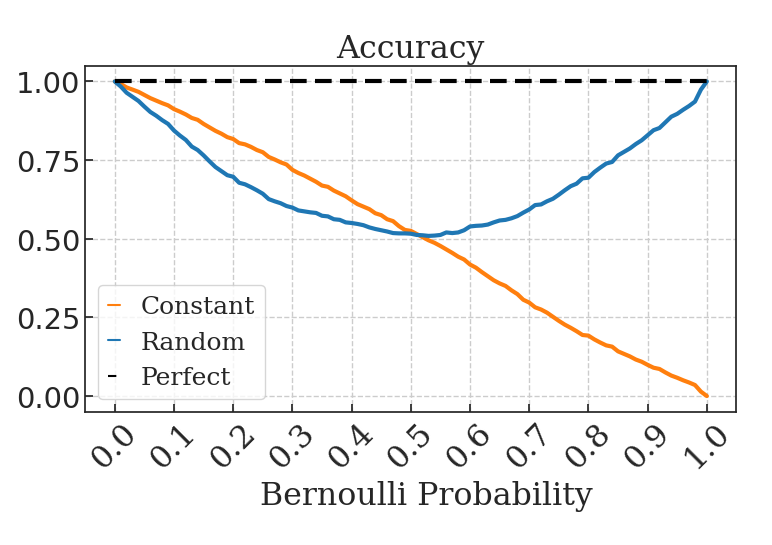
\includegraphics[width=\textwidth]{img/results_discussion/empirical/artificial_acc_final.png}
    \end{subfigure}
    \hfill
    \begin{subfigure}[b]{0.45\textwidth}
        \centering
        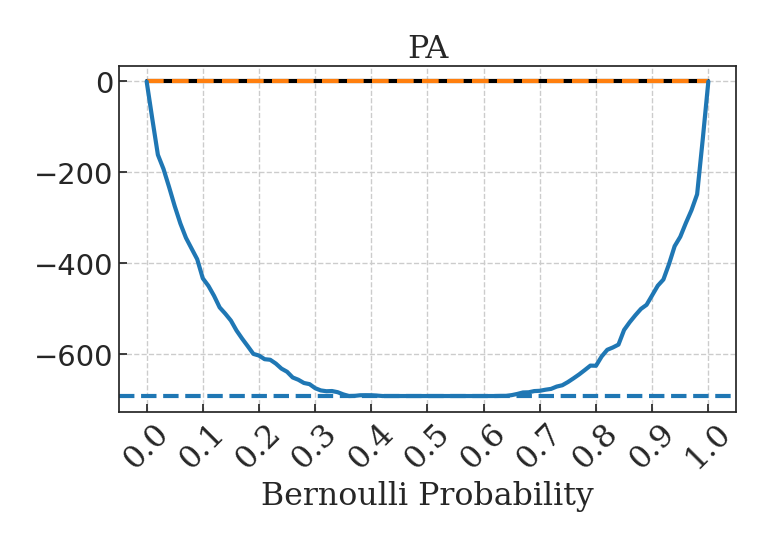
\includegraphics[width=\textwidth]{img/results_discussion/empirical/artificial_logPA_final.png}
    \end{subfigure}
    \caption{
    Evolution of PA and accuracy for constant, perfect and random classifiers across different 
    values of $p \in [0,1]$. Accuracy does not comply with the desired properties of a robustness metric
    and provides an inconsistent assessment that is exclusively driven by task performance. In contrast,
    PA continuously discriminates robust from unrobust classifiers for $p \in (0,1)$ and reaches 
    its minimum (blue dashed line) for the random classifier when $p \in (0.3,0.7)$.
    }
    \label{fig:empirical_plot}
\end{figure}

Table \ref{tab:empirical_table} displays the values of PA and accuracy
obtained for the case $p = 1/2$. It is clear that PA is independent of the task performance
of the model, which in classification tasks is mostly reported through accuracy-based metrics, and 
instead discriminates effectively the random classifier from the rest. In particular, 
PA converges towards its minimum value $-N \log{2}$ for the random classifier 
as $\beta \longrightarrow 0$, and converges towards zero for the 
other two as $\beta \longrightarrow \infty$. This behavior aligns with the 
intuitive assessment given in Example \ref{example:robustness}, since perfect and constant 
classifiers are robust by definition, while random classifiers are extremely unrobust. \\

 It can be observed that the miniumum PA is obtained only after 
a certain mismatch threshold has been reached, of approximately 30\% of the samples. 
This illustrates the trade-off navigated during $\beta$ optimization, in which 
matching samples are more heavily penalized the higher the value of $\beta$ is,
whereas mismatching samples are more heavily penalized the lower the value of $\beta$ is.
A balanced random classifier (i.e. balanced on the two classes) would yield the minimum
PA value for any possible original sample, as shown in the blue dashed line.\\

Figure \ref{fig:empirical_plot} extends these results across different values of 
$p \in [0,1]$. It can be observed that the minimum PA is obtained only after a mismatch 
threshold of approximately 30\% of the samples has been reached. This illustrates the 
trade-off navigated during $\beta$ optimization, where matching samples are increasingly penalized 
as the value of $\beta$ increases, while mismatching samples are more heavily penalized 
as $\beta$ decreases. FINISH. \\

The prediction confidence, expressed as a difference in  the unnormalized log-odds $\bm{F}$, 
is very informative with regard to the quality of the model, as we can intuitively infer that the latent 
space represented by a high-confidence model encodes a better set of features 
to discriminate observation classes than one with a lower prediction confidence. \\

HERE INTERPRETATION OF INFORMATIVENESS AND BETA. ALSO HERE INTERPRETATION OF BETA CONVERGENCE AND 
WHY WE DONT SET THE VALUE TO ZERO. HERE INTERPRETATION OF INFORMATIVENESS AND BETA. 
ALSO HERE INTERPRETATION OF BETA CONVERGENCE AND WHY WE DONT SET THE VALUE TO ZERO.
These and other results (see Appendix \ref{subsec:appendix_empirical_behaviour}) indicate
that the PA kernel behaves as expected and is highly informative of the generalization
capabilities of the model, provided that the nature of the randomness existing
between $\bm{x}^\prime$ and $\bm{x}^{\prime \prime}$ is known. \\

\begin{figure}[t]
    \centering
    \begin{subfigure}[b]{0.45\textwidth}
        \centering
        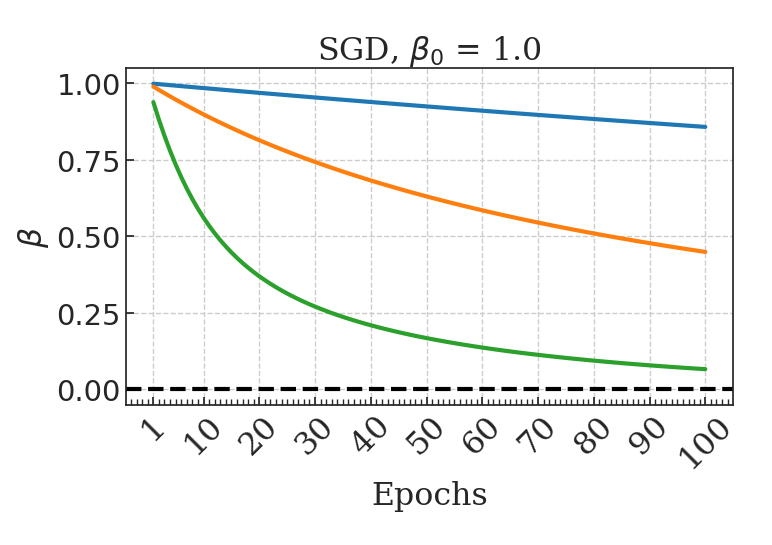
\includegraphics[width=\textwidth]{img/results_discussion/empirical/nonrob_met=betas_hue=ldiff.png}
    \end{subfigure}
    \hfill
    \begin{subfigure}[b]{0.45\textwidth}
        \centering
        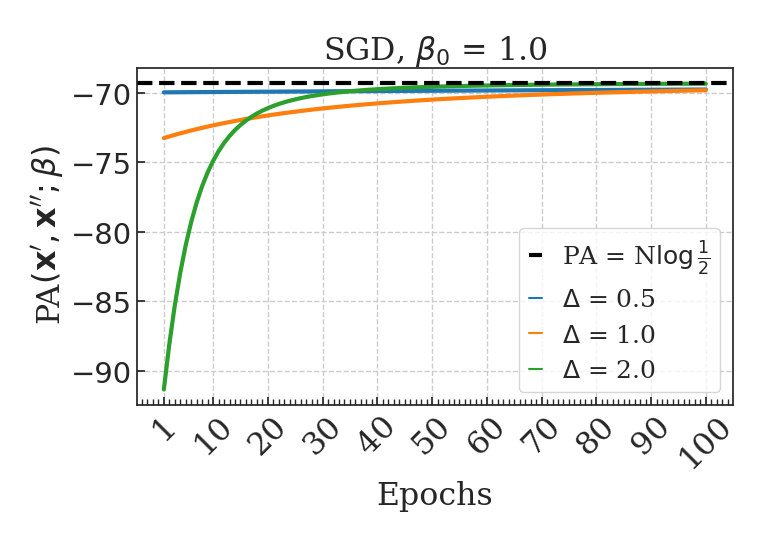
\includegraphics[width=\textwidth]{img/results_discussion/empirical/nonrob_met=logPA_hue=ldiff.png}
    \end{subfigure}
    \caption{Evolution of PA kernel optimization under different levels of prediction 
    confidence. An illustration of the original log-odds and its associated posterior distribution
    can be found in Appendix \ref{subsec:appendix_empirical_behaviour}.}
    \label{fig:prediction_confidence}
\end{figure}

The results obtained with artificial samples motivate the exploration of more realistic
scenarios. In general, the PA metric is expected to capture the generalization capabilities
of any model yielding probabilistic predictions, regardless of the task at hand. This
already represents an incredible advantage from an epistemological perspective, as we
can argue that the metric is agnostic of the underlying mechanism that generated the data
and even to the nature of the data itself. \\

In order to verify this claim, we will start by evaluating the robustness of two
different classifier models in two different domains under increasing levels of 
random noise. This particular setting, even if synthetically designed, is 
relevant in any classification context because it provides a general measure of the 
quality of the features learned. The presence of noise, at least 
at low levels, does not perturb the set of features that define a particular class from
a perceptual standpoint and should therefore not perturb very significantly the
predictions of robust models.

\begin{experiment}
The model under consideration is an image classifier for CIFAR10, a popular
computer vision dataset composed of coloured, 32 $\times$ 32 pixel images belonging to 10
different classes \cite{krizhevskyLearningMultipleLayers}. Sample
$\bm{x}'$ contains 10.000 images and $\bm{x}''$ is generated 
by perturbing each image with white noise of increasing intensity.
A pre-trained, undefended WideResNet-28-10
\cite{BMVC2016_87}
architecture is used to evaluate the effectiveness of the attack. The 
magnitude of the perturbations is expressed in the same terms as those 
of an adversarial attack for further reference, but translate to 
using $\sigma = 3 \ell_\infty$, as 99.73\% of the
total mass of the gaussian distribution lies within the 
interval $\pm 3\sigma$.
\end{experiment}

\begin{figure}[b]
    \centering
    \begin{subfigure}[b]{0.45\textwidth}
        \centering
        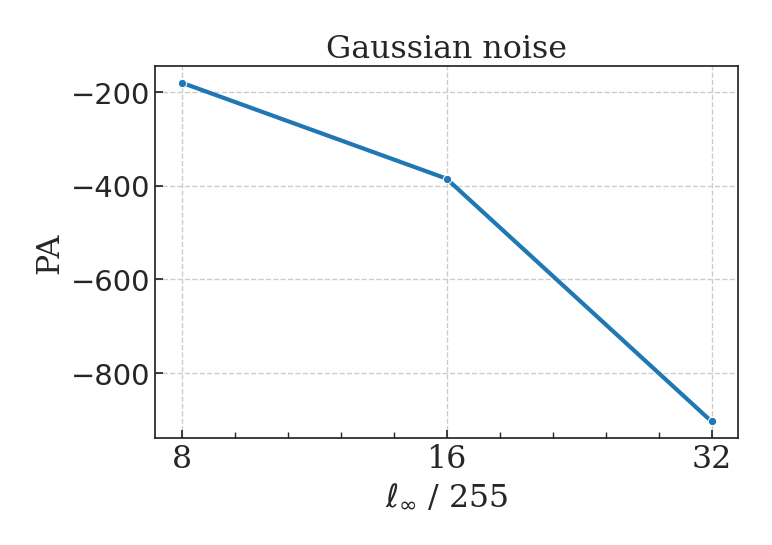
\includegraphics[width=\textwidth]{img/results_discussion/adversarial/GAUSSIAN_logPA_eps_single.png}
    \end{subfigure}
    \hfill
    \begin{subfigure}[b]{0.45\textwidth}
        \centering
        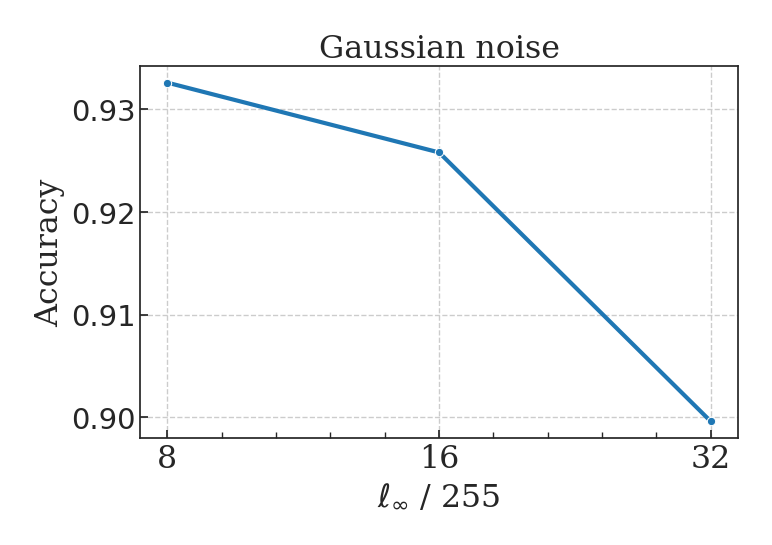
\includegraphics[width=\textwidth]{img/results_discussion/adversarial/GAUSSIAN_acc_pa_eps_single.png}
    \end{subfigure}
    \caption{PA and accuracy displayed by the CIFAR10 classifier under increasing levels of white noise. Robustness
    and task performance are shown to be non-linearly related.
    }
    \label{fig:gaussian_noise}
\end{figure}



Figure \ref{fig:gaussian_noise} shows that 
PA is highly sensitive to the presence of white noise and effectively captures the factor 
of increase in the magnitude of the perturbations. In general, gaussian perturbations genuinely simulate increasing levels of sampling randomness, as the 
perceptual features that should drive the inductive bias of the model are still present, even 
if in a proportionally dissimilar way as they were encoded. In contrast to adversarial attacks, 
these perturbations are not expected to distort the predictive outcome 
abruptly. As a result, any robustness score will be driven by the standard generalization error, including validation 
accuracy. \\

Figure \ref{fig:gaussian_optimization} expands these results by gradually adjusting
the perturbation so that it only affects a specific ratio of observations. As expected, 
$\beta \longrightarrow \infty$ in the unperturbed case, and converges
quickly to its optimal value in the rest of cases, even for a considerably large 
sample size. The decay in the PA value is less pronounced the higher
fraction of perturbed samples are there, which is consistent with the concept 
of robustness defined, as it already approaches the lower bound for these kinds of 
perturbation even when the whole sample has yet not been affected. \\


\begin{figure}[t]
    \centering
    \begin{subfigure}[b]{0.49\textwidth}
        \centering
        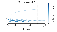
\includegraphics[width=\textwidth]{img/results_discussion/empirical/beta_100.pdf}
    \end{subfigure}
    \hfill
    \begin{subfigure}[b]{0.49\textwidth}
        \centering
        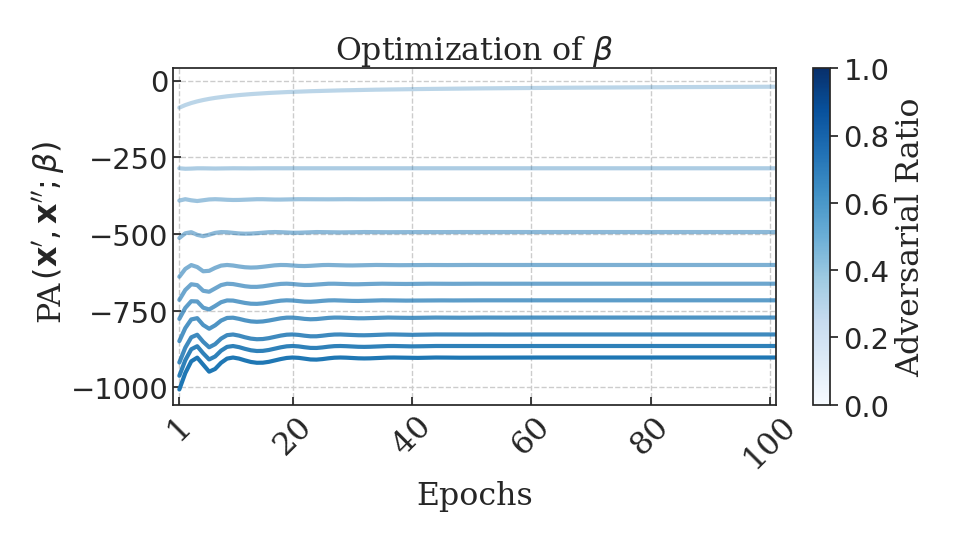
\includegraphics[width=\textwidth]{img/results_discussion/empirical/logPA_100.png}
    \end{subfigure}
    \caption{PA kernel optimization in the CIFAR10 gaussian noise setting for different ratio
    of perturbed samples. Perturbation magnitude is $\ell_\infty$ = 32 / 255.}
    \label{fig:gaussian_optimization}
\end{figure}



\begin{experiment}
The model under consideration is a sentiment classifier for IMDB,
a popular NLP dataset containing 50,000 movie reviews labeled 
as either positive or negative
\cite{maas2011learning}. 
A pre-trained DistilBERT-based architecture 
is adopted, with the appropiate tokenizer
\cite{sanh2019distilbert}. 
After a 100 epoch training using SGD with a learning rate of $10^{-3}$, the model with the highest validation
accuracy is selected. Then, the original test dataset $\bm{x}^\prime$
is incrementally perturbed to generate $\bm{x}^{\prime \prime}$, by either adding, removing or replacing 
single characters. This perturbation amounts to increasing the Levenshtein
distance $L$ between identical observations of the dataset, and the attack power
is defined as $2^{L}$.
\end{experiment}

\begin{figure}[b]
    \centering
    \begin{subfigure}[b]{0.45\textwidth}
        \centering
        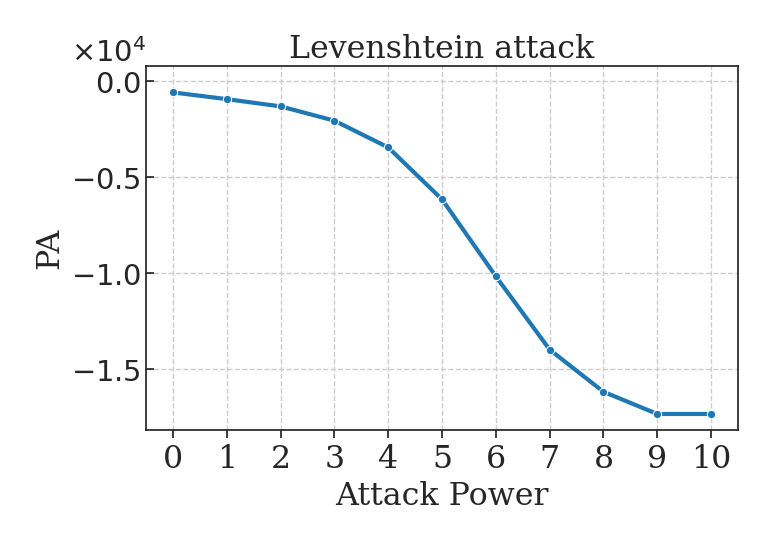
\includegraphics[width=\textwidth]{img/results_discussion/empirical/levenshtein_logPA.png}
    \end{subfigure}
    \hfill
    \begin{subfigure}[b]{0.45\textwidth}
        \centering
        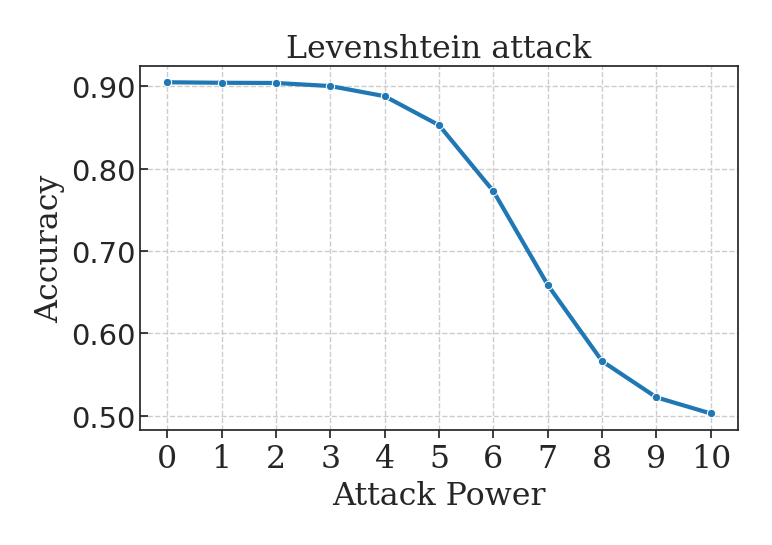
\includegraphics[width=\textwidth]{img/results_discussion/empirical/levenshtein_AFR_true.png}
    \end{subfigure}
    \caption{PA and accuracy for the IMDB sentiment classification under Levenshtein perturbations.
    The attack power is defined as $2^L$, being $L$ the Levenshtein distance between pairs of
    observations in $\bm{x}^\prime$ and $\bm{x}^{\prime\prime}$.}
    \label{fig:imdb_levenshtein}
\end{figure}

Figure \ref{fig:imdb_levenshtein} shows that PA is highly sensitive to the
presence of Levenshtein perturbations, as it is able to capture the
change in the predictive outcome of the model even when performance remains 
unaltered. In particular, accuracy remains maximum even when 4 characters
are perturbed in every observation, and begins to decrease only after that. In contrast,
PA drops significantly after the first perturbation and reaches its minimum value
after $2^9$ perturbations have been made, indicating that the outcome is maximally
unrobust. \\

Further discrepancies between accuracy and PA can be observed if the 
attack is designed to directly influence the sentiment prediction, which corresponds
to an adversarial setting. For instance, Figure \ref{fig:imdb_adversarial} shows that accuracy can be 
manipulated to increase or decrease by perturbing original samples with
adjectives that reinforce or contradict, respectively, 
the sentiment expressed in the review. In both cases, PA measures the lack of robustness in the
predictions that these perturbations represent, regardless of the task
performance displayed. The robustness against of adversarial attacks in
image classification tasks will be discussed in the next section. \\

\section{Adversarial setting}\label{sec:results_adversarial}

The first scenario in which covariate shift robustness will be measured is the
adversarial case. This setting serves as an archetypal use case for a robustness 
metric, given that adversarial perturbations are deliberately generated to mislead the
model, and any robustness score will ultimately be driven by the effectiveness of the 
attack. In particular, PA should be highly informative about the defensive capabilities 
of models, as the posterior distribution over the hypothesis class will shift 
significantly in the presence of adversarial perturbations. This section aims to validate 
this claim and provide deeper insights into the nature of the metric. \\

It is important to note that adversarial perturbations constitute an
intermediate instance between sampling randomness and distribution shift. 
On the one hand, they emulate a sampling variation that appears 
as an outlier under the model's representation of the true class, even if
the source of variability is completely artificial. On the other
hand, samples are known to contain the set of features that should 
align with the inductive bias of the model, and so the model's ability to 
distillate those features is in question. In practice, we are evaluating the 
quality of the complex discriminator function defining a basin of stability
around original samples, and for that no deep understanding of the nature of 
the randomness of the samples or the features they encode is needed.\\

This interpretation is aligned with the measure provided by accuracy-based metrics, 
because adversarial examples do not entail any accountable source of randomness, 
but instead exploit specific vulnerabilities of models to alter the position of the 
maximum of the posterior ditribution. A greater posterior overlap will still
indicate higher robustness to attacks, regardless of the nature of the model or the
attack, but optimal posteriors are expected to converge to very peaked gibbs
distributions centered at the predicted class, reducing the interpretability of PA
to that of accuracy. \\

In order to explore these claims, robustness and performance results will be
provided through the attack failure rate (AFR) value and compared to those
yielded by PA. The AFR computed with the true class labels will be used as a baseline
of model performance, whereas the AFR computed with the predicted class label
will be a reference for robustness, as it aligns with the aforementioned
interpretation.

\begin{definition}[\emph{Attack failure rate}]
    Let $\bm{\hat{y}^\prime}, \bm{\hat{y}^{\prime\prime}} \in \mathcal{Y}^N$ be the predicted class 
    labels for $\bm{x}^\prime$ and $\bm{x}^{\prime \prime}$, respectively, 
    and let $\bm{y}\in \mathcal{Y}^N$ be the true labels. Considering the definition of accuracy
    provided in Section \ref{sec:robustness_to_covariate_shift}, the attack failure rate (AFR)
    can be expressed as

    $$
    \begin{aligned}
        \operatorname{AFR}_\text{T} &= \operatorname{Accuracy}(\bm{\hat{y}^{\prime \prime}}, \bm{y}), \\
        \operatorname{AFR}_\text{P} &= \operatorname{Accuracy}(\bm{\hat{y}^{\prime \prime}}, \bm{\hat{y}^{\prime}}).
    \end{aligned}
    $$

\end{definition}

\begin{definition}[\emph{Adversarial ratio}]
    Besides the maximum norm allowed for each perturbation, we are also interested in evaluating 
    the sensitivity of our robustness measure to the ratio of perturbed samples in the dataset, 
    also known as adversarial ratio $\alpha \in [0,1]$. The final adversarial dataset $\bm{x}''$ will be generated as

    $$
    \bm{x}'' := \alpha \bm{x}'' + (1 - \alpha) \bm{x}',
    $$

    where $\bm{x}'' = \bm{x}' + \bm{\Delta}$, as per Definition \ref{def:adversarial_perturbation}.
\end{definition}

This incremental expansion of the attack is particularly relevant for PA, as we would initially 
expect it to behave non-linearly with respect to $\alpha$ and converge faster to
the the $\alpha=1$ robustness value than any accuracy-based metric, in light of the results obtained
in the previous section. \\

Before delving into the results, it is worth exploring the immediate consequences
of the previous claim, namely the fact that the maximum posterior agreement will
be achieved when gibbs distributions are highly peaked on the predicted 
class, at least for moderate attacks. This is because most adversarial 
perturbations will not succeed at misleading the model and thus drive the inverse temperature to
infinity. The divergence of $\beta^{*}$ is only limited by the set of misleading adversarial 
examples, that for being perturbed from the original class are still expected to assign a
significant confidence to the original prediction, even if not the maximum anymore.
Table \ref{tab:entropy_gibbs} illustrates this claim by showing that $\beta^{*} > 1$ 
for all robust models, resulting in a substantial decrease of the entropy between initial and 
optimal posteriors. \\

This realization allows us to break down the dataset into subsets of observations
that contribute to the final PA value in different ways, and therefore improve
the interpretation of the resulting robustness measurement.
For a start, a robust model should be expected to correctly classify most of the 
original observations with high confidence, as they
contain the features encoded in the inductive bias of the 
classifier. Original samples that do not contain these features will be misclassified,
and the lack of generalization to sampling randomness should be penalized for lowering
the confidence in the predicted class. Regarding adversarial examples, a clear
distinction between robust and non-robust models should be made based on the success 
rate of perturbations and the confidence attributed to misleading predictions. Adversarial 
perturbations on originally misclassified observations will not be of much interest,
as the effect on prediction confidence should not be as significant as in
the correctly classified ones. An interpretable expression for PA in the adversarial
setting can be obained by approximating the optimal posterior for each of these
subsets of observations. \\

\begin{theorem}[\emph{Approximated PA in the adversarial setting}]
    Let $\Xi_{\text{ERR}}$, $\Xi_{\text{MIS}}$ and $\Xi_{\text{ADV}}$ be the approximated robustness
    contributions of correctly classified original samples, misclassified original samples
    and misleading adversarial samples, respectively. Then, we can express

    $$
    \operatorname{PA} \approx \Xi_{\text{ERR}} + \Xi_{\text{MIS}} + \Xi_{\text{ADV}} = \Xi_{\text{SAM}} + \Xi_{\text{ADV}} 
    $$

    with
    $$
    \begin{aligned}
        &\Xi_{\text{ERR}} = N \operatorname{AFR}_T^0 \operatorname{AFR}_P \log \left( 1 - 2\delta_{\text{ERR}} \right), \\
        &\Xi_{\text{MIS}} = N (1- \operatorname{AFR}_T^0) \operatorname{AFR}_P \log \left( 1 - 2\delta_{\text{MIS}} \right), \\
        &\Xi_{\text{ADV}} = N \operatorname{AFR}_T^0 (1 - \operatorname{AFR}_P) \log \delta_{\text{ADV}},
    \end{aligned}
    $$

    where $\operatorname{AFR}_T^0 \equiv \operatorname{AFR}_T(\alpha=0)$ is the accuracy of the model in the original data.
    Variables $\delta_{\text{ERR}}$, $\delta_{\text{MIS}}$ and $\delta_{\text{ADV}}$ account for the 
    average probability assigned to
    classes other than the predicted class for the three aforementioned cases 
    (see illustration in Figure \ref{fig:appendix_adv_illustration}). $\Xi_{\text{SAM}}$ aggregates
    the first two terms and will be interpreted as the sampling randomness contribution.
    \label{thm:approximated_pa}
\end{theorem}
\begin{proof}
    See Apendix \ref{sec:appendix_results_adversarial}.
\end{proof}

Figures \ref{fig:appendix_adversarial_approx_pa_pgd} and \ref{fig:appendix_adversarial_approx_pa_fmn}
compare the true and approximated PA values under increasing adversarial ratio for
PGD and FMN attacks, respectively. It is clear that penalizations are overestimated, 
given that the average posterior probability was used and differences by defect are more 
significantly penalized than those by excess due to the nonlinear nature of the logarithm in 
the range $[0,1]$. Besides, $\beta^{*}$ is fixed to its lowest possible value (i.e. when $\alpha$ = 1),
which makes the approximation on the FMN attack less reliable for smaller adversarial 
ratio settings, as $\beta^{*}$ decreases significantly due to the effectiveness of the attack. \\

Nevertheless, the relative differences in the approximated PA values are consistent
with the true values, and the ranking of the models is largely preserved across different
$\alpha$ values. For that reason, the additional interpretability provided by this approximation
will illustrat PA expression will help characterize the source of the robust and unrobust
observed in the different models. \\

\begin{table}[t]
    \centering
        \begin{tabular}{l|rr|rr}
        Defense & $\beta^{*}_{\text{PGD}}$ & $\Delta H_{\text{PGD}}$  & $\beta^{*}_{\text{FMN}}$ & $\Delta H_{\text{FMN}}$ \\
        \midrule
        {\color{tab:orange} \textbf{Undefended}} & 0.78 & 0.048 & 0.65 & 0.10\\
        {\color{tab:blue} \textbf{Engstrom et al.}} & 15.63 & -1.204 & 2.59 & -0.71\\
        {\color{tab:green} \textbf{Athalye et al.}} & 35.48 & -3.049 & 19.84 & -2.13 \\
        {\color{tab:red} \textbf{Wong et al.}} & 15.46 & -1.229 & 4.59 & -0.96\\
        {\color{tab:purple} \textbf{Addepalli et al.}} & 15.89 & -2.023 & 6.08 & -1.71 \\
        {\color{tab:brown} \textbf{Wang et al.}} & 11.24 & -1.833 & 2.53 & -1.41\\
        \bottomrule
        \end{tabular}
        \caption{
        Entropy difference $\Delta H = H(\beta^{*}) - H(1)$
        for different models, obtained for FMN and $\ell_\infty$ = 8/255 
        PGD attacks, both at $\alpha = 1$. Entropy values are 
        estimated using the average posterior distribution over correctly classified
        samples, which constitute the largest proportion of the dataset.
        Figures \ref{fig:pgd_distributions_undefended}-\ref{fig:pgd_distributions_bpda}
        show the initial and optimal average posteriors from which these values
        were computed.
        }
        \label{tab:entropy_gibbs}
\end{table}

\begin{experiment}
The results provided in this section have been obtained using the CIFAR10 dataset
\cite{krizhevskyLearningMultipleLayers},
which is widely regarded as a standard benchmark for robustness evaluation. CIFAR10 is
a balanced dataset containing 60.000 coloured 32 $\times$ 32 pixel images belonging to 10
different classes. We will consider a pre-trained WideResNet-28-10
\cite{BMVC2016_87}
as a baseline, undefended model and compare it to some state-of-the-art robust ResNet50
\cite{resnet50}
models provided by the 
RobustBench \cite{croceRobustBenchStandardizedAdversarial2021a}
library under PGD \cite{madryDeepLearningModels2019}
and FMN \cite{pintorFastMinimumnormAdversarial2021}
attacks, both run for 1000 steps (see Section \ref{sec:adversarial_setting}).
The defenses applied are those proposed by 
{\color{tab:blue} \textbf{Engstrom et al.}} \cite{engstrom2019adversarial}, 
{\color{tab:green} \textbf{Athalye et al.}} \cite{AthalyeC018}, 
{\color{tab:red} \textbf{Wong et al.}} \cite{WongRK20}, 
{\color{tab:purple} \textbf{Addepalli et al.}} \cite{Addepalli2022ScalingAT}
and {\color{tab:brown} \textbf{Wang et al.}} \cite{wang2023betterdiffusionmodelsimprove}.
The PGD attack power will be specified in terms of $\ell_\infty$, which corresponds
to the maximum perturbation allowed for each pixel. This is consistent with the characterization
of adversarial perturbation given in the previous chapter, as every perturbation will be bounded
to the region defined by $\mathbf{B}_\infty^{\ell_{\infty}} (x)$.
\end{experiment}

\begin{figure}[H]
    \centering
    \begin{subfigure}[b]{0.25\textwidth}
        \centering
        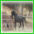
\includegraphics[width=\textwidth]{img/results_discussion/adversarial/adv_unperturbed_framed.png}
        \caption{Original}
    \end{subfigure}
    \hfill
    \begin{subfigure}[b]{0.25\textwidth}
        \centering
        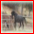
\includegraphics[width=\textwidth]{img/results_discussion/adversarial/adv_pgd_framed.png}
        \caption{PGD, $\ell_\infty$ = 36/255}
    \end{subfigure}
    \hfill
    \begin{subfigure}[b]{0.25\textwidth}
        \centering
        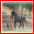
\includegraphics[width=\textwidth]{img/results_discussion/adversarial/adv_fmn_framed.png}
        \caption{FMN}
    \end{subfigure}
    \caption{Original and adversarially-perturbed CIFAR10 sample of class \texttt{horse}. Both perturbations succeed
    at misleading an undefended, pre-trained WideResNet-28-10 architecture.}
\end{figure}

The first results presented correspond to PGD attacks with different attack power 
$\ell_\infty$, namely 8/255, 16/255 and 32/255, for increasing ratio of 
perturbed samples in the CIFAR10 dataset.

\begin{figure}[H]
    \centering
    \begin{subfigure}[b]{\textwidth}
        \centering
        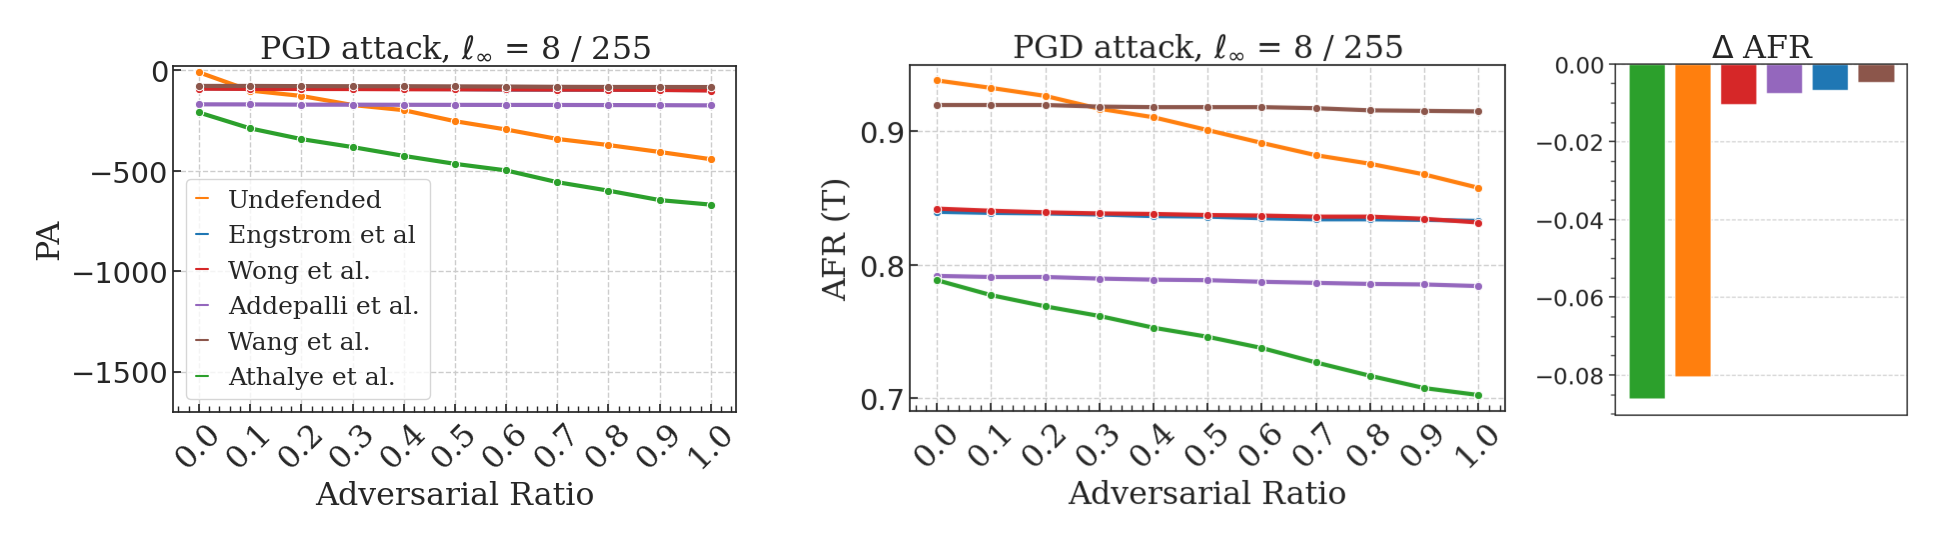
\includegraphics[width=\textwidth]{img/results_discussion/adversarial/PGD_0.0314_combo.png}
    \end{subfigure}

    \vspace{1em}

    \begin{subfigure}[b]{\textwidth}
        \centering
        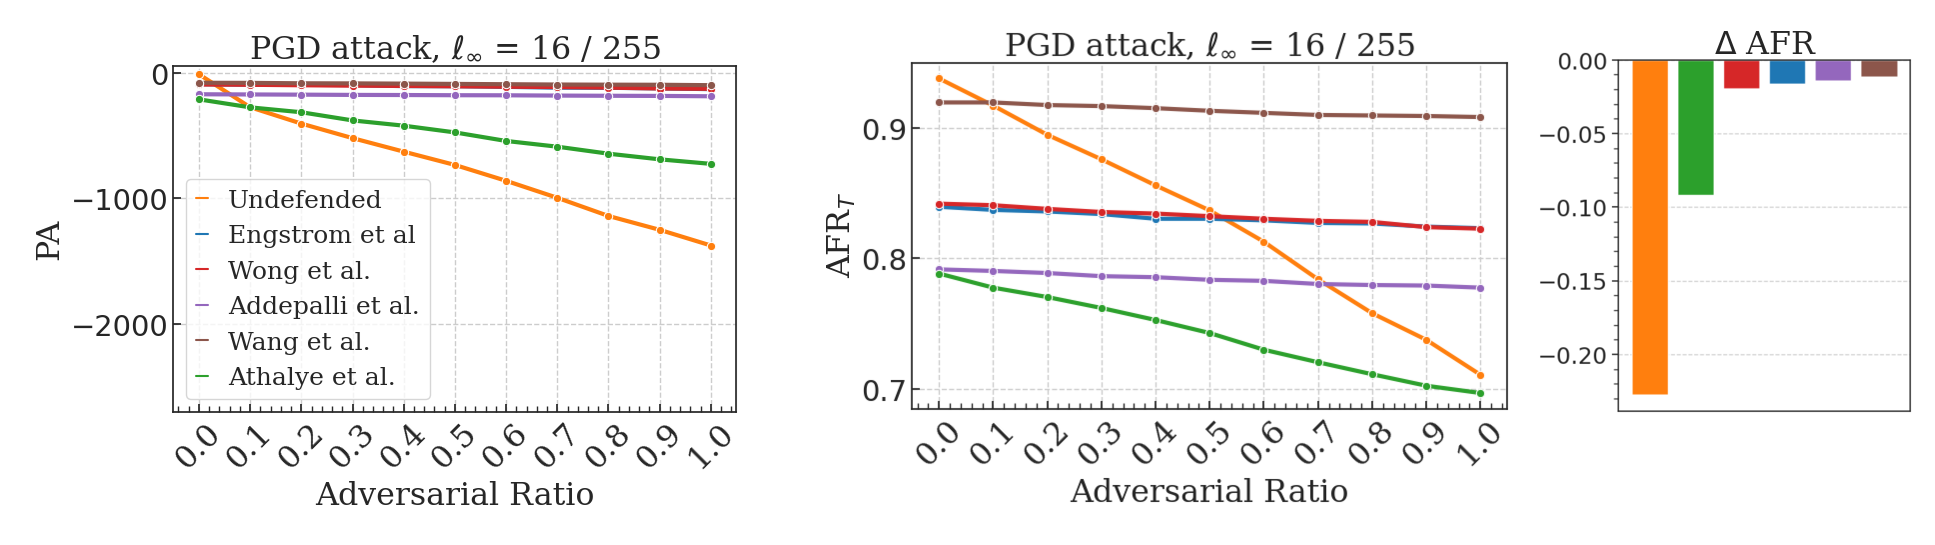
\includegraphics[width=\textwidth]{img/results_discussion/adversarial/PGD_0.0627_combo.png}
    \end{subfigure}

    \vspace{1em}

    \begin{subfigure}[b]{\textwidth}
        \centering
        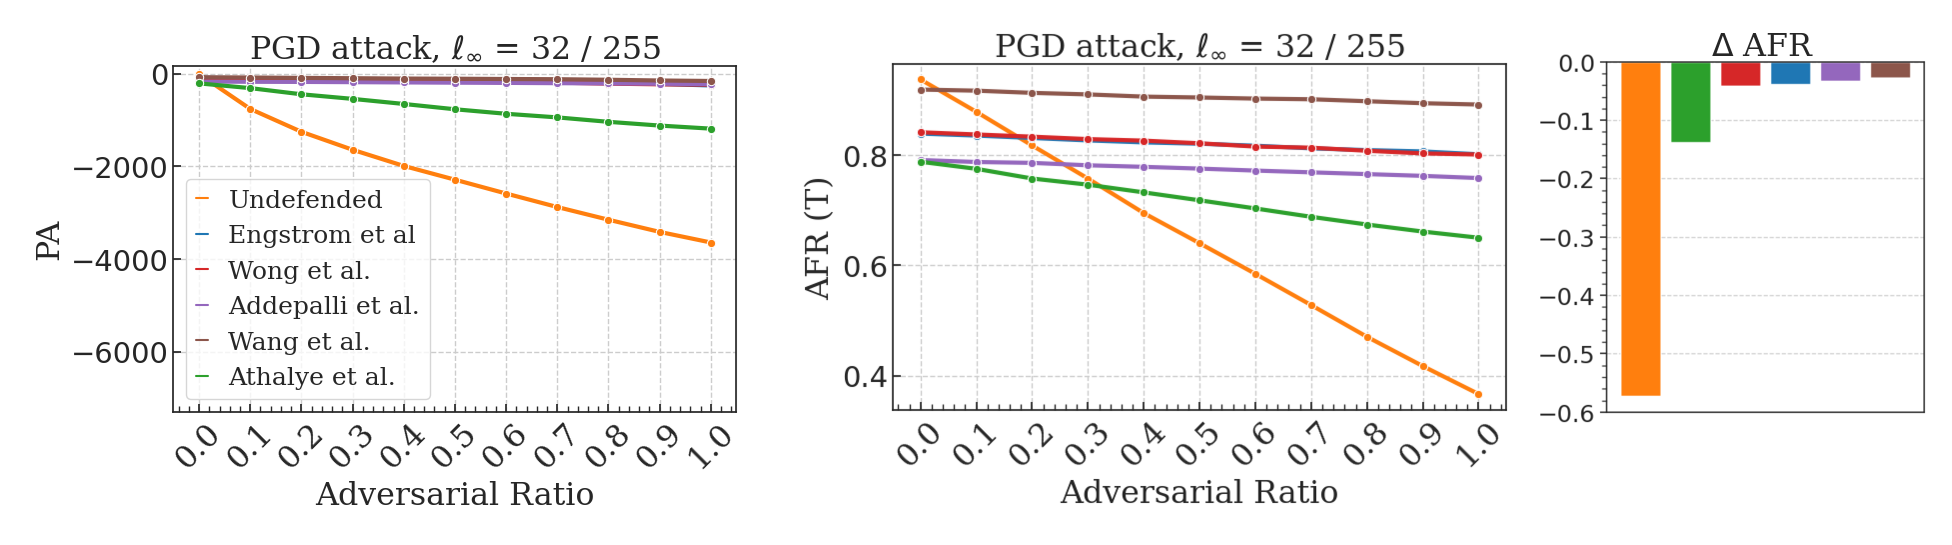
\includegraphics[width=\textwidth]{img/results_discussion/adversarial/PGD_0.1255_combo.png}
    \end{subfigure}

    \caption{PA, $\operatorname{AFR}_\text{T}$ and the AFR variation against increasing adversarial ratio $\alpha \in [0,1]$ at different
    perturbation norm bounds $\ell_infty$. A pre-trained, undefended WideResNet-28-10
    and five RobustBench %\cite{croceRobustBenchStandardizedAdversarial2021a}
    defended models are subject to a 1000 step PGD attack.
    When $\alpha$ = 0, $\operatorname{PA} \longrightarrow 0$ as $\beta \longrightarrow \infty$ in all cases, but
    the convergence rate depends on the prediction confidence (see Figure \ref{fig:prediction_confidence}) and thus yields an assessment equivalent to that
    of $\operatorname{AFR}_\text{T}$.
    }
    \label{fig:six_figures_pa_adv}
\end{figure}

At first glance, it is clear that PA is able to discriminate robust models from
the {\color{tab:orange} \textbf{Undefended}} one, which is shown to significantly
decrease its performance with increasing adversarial ratio and attack power. As expected, 
the rate at which its performance decreases is higher
the more powerful the attack is, since a greater percentage of samples are able to
mislead its predictions. \\

From both PA and $\operatorname{AFR}_{\text{T}}$ stems the fact that {\color{tab:green} \textbf{Athalye et al.}}
is significantly less robust to PGD attacks than its RobustBench counterparts, as 
its performance decreases way more significantly with increasing adversarial ratio. 
We observe that the rate at which its performance decreases is inversely proportional to the 
attack power. This is consistent with the behaviour expected from a JPEG compression defense 
mechanism, as it is less effective for small perturbations \cite{dasKeepingBadGuys2017}. \\

A fundamental difference between these two models, which cannot be
inferred from a purely performance-based metric, is the nature of the misalignment in
the probabilistic output of the model, which is the source of the robust and non-robust
behaviour observed. Figure \ref{fig:unrobust_posterior_short_pgd} \textbf{(right)}
shows the optimal $\beta^{*}$ value for each model, which follows
the entropy of the posterior distribution and discriminates the two non-robust
models from the rest and from each other. The {\color{tab:orange} \textbf{Undefended}}
model provides overconfident predictions that maximize disagreement in misleading and 
misclassified samples, whereas {\color{tab:green} \textbf{Athalye et al.}} provides 
uncertain predictions that minimize disagreement in adversarial samples but have 
the opposite effect in correctly classified ones. \\

Following the interpretation outlined in Chapter \ref{sec:theory}, we show that $\beta^{*}$ effectively measures the quality of 
the informativeness estimation made by each model. The {\color{tab:orange} \textbf{Undefended}} 
model overestimates the information content of the features it has learned, and thus overfits 
to these and is unable to generalize under adversarial perturbations. On the other hand, 
{\color{tab:green} \textbf{Athalye et al.}} underestimates the information content and thus
provides overly uncertain predictions. The maximum mutual information between posteriors is 
lower than its robust counterparts for both models, the former because information is not 
mutual and the latter because there is less information.
This insight clarifies the unintuitive behaviour observed earlier, by which {\color{tab:green} \textbf{Athalye et al.}} 
robustness value decreases at a lower rate with increasing attack power, despite maintaining a
constant decrease in performance. \\

Figure \ref{fig:unrobust_posterior_short_pgd} \textbf{(left)} illustrates
the previous reasoning by displaying the average posterior
probability assigned to the predicted class by each model, conditioned on the type
of prediction assigned. This discrimination yields three groups of observations,
namely original samples that are correctly classified by the robust model, 
original samples that are misclassified, and perturbed samples that, having their 
associated unperturbed sample been correctly classified, 
have been able to mislead the model. These three cases are relevant from the 
adversarial robustness perspective,  as they illustrate the trade-off between high-confident 
original predictions and adversarial vulnerability, which has been already stated in 
previous chapters. {\color{tab:brown} \textbf{Wang et al.}}
acts as a reference for an ideal robust behaviour, in which original samples are
predicted with high confidence and adversarially misleading predicted labels are 
only slightly more likely than the rest. Equivalent representations for the remaining
models can be found in Figure \ref{fig:appendix_adversarial_distribution_pgd}.\\

\begin{figure}[H]
    \centering
    \begin{subfigure}[b]{\textwidth}
        \centering
        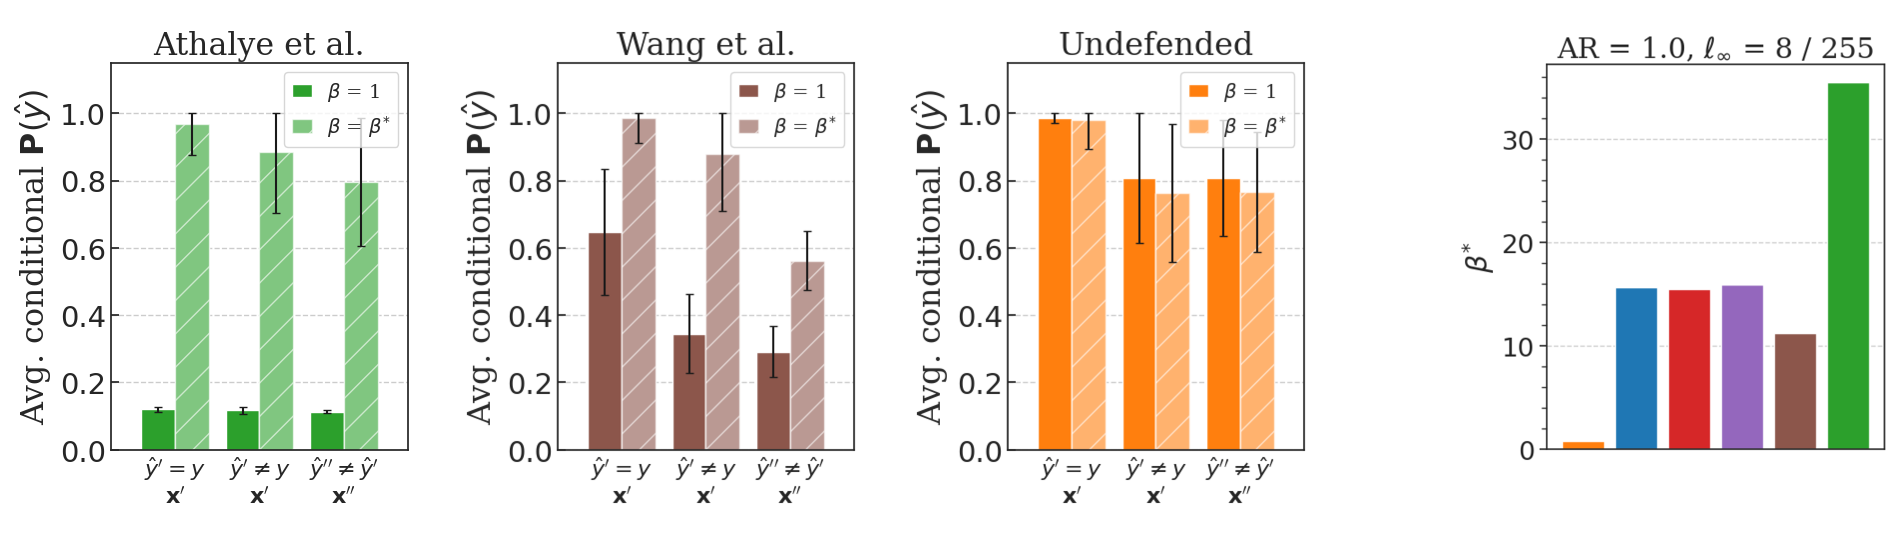
\includegraphics[width=\textwidth]{img/results_discussion/adversarial/bpda_wang_undefended_beta_pgd.png}
    \end{subfigure}
   
    \caption{(\textbf{left}) Average posterior probability of the predicted class for 
    correctly classified original samples, misclassified original samples, and 
    misleading adversarial samples, respectively. (\textbf{right}) Optimal $\beta^{*}$ value for each model.
    Results obtained through a PGD attack with $\ell_\infty = 8 / 255$.}
    \label{fig:unrobust_posterior_short_pgd}
\end{figure}

With respect to robust models, we observe a significant difference in the 
discriminative power of PA and accuracy-based metrics that does not immediately
derive from the informativeness of the optimal posterior. As remarked before, AFR (P)
constitutes our baseline robustness metric, as by definition represents the ratio
of predictions that remained constant under adversarial perturbations, and
therefore ranks models by their predictive capabilities against these attacks. The
value of $\Delta$AFR aligns with that definition, and discriminates robust models
by a very thin margin, selecting {\color{tab:brown} \textbf{Wang et al.}} as
the best. Further analysis on PA is needed to understand the source of this 
discrepancy, as for instance why {\color{tab:purple} \textbf{Addepalli et al.}} model
is attributed a significantly lower value than the remaining robust models
under a $\ell_\infty$ = 8/255 PGD attack, despite displaying a similar decrease in performance. \\

\begin{figure}[H]
    \centering
    \begin{subfigure}[b]{0.37\textwidth}
        \centering
        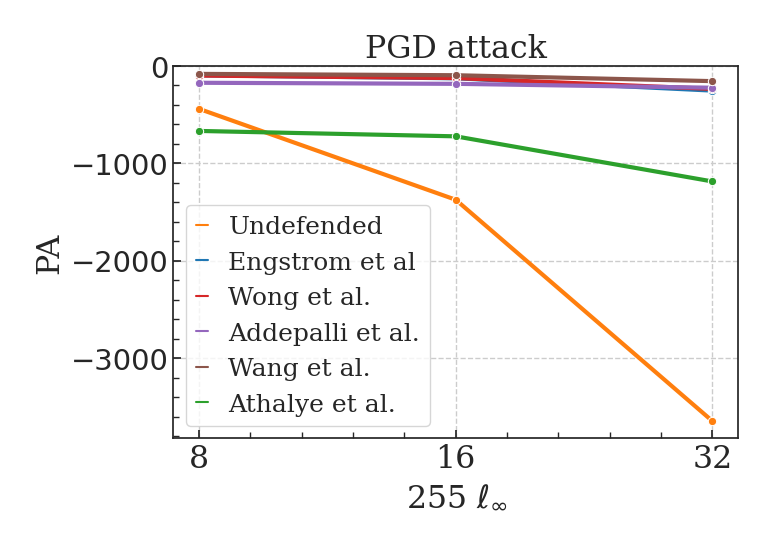
\includegraphics[width=\textwidth]{img/results_discussion/adversarial/PGD_logPA_eps.png}
    \end{subfigure}
    \hfill
    \begin{subfigure}[b]{0.59\textwidth}
        \centering
        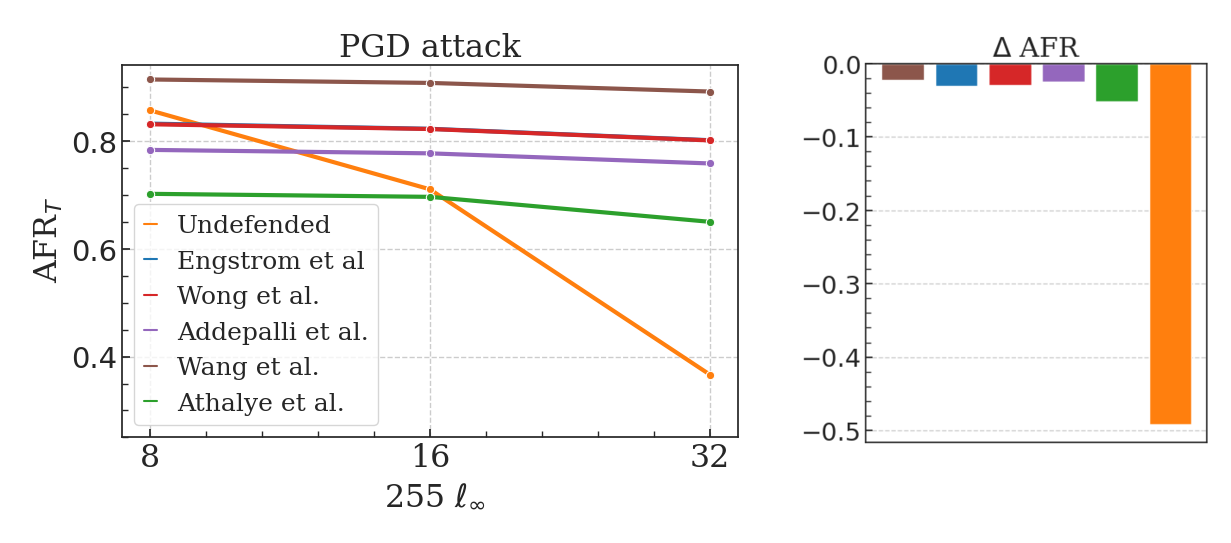
\includegraphics[width=\textwidth]{img/results_discussion/adversarial/PGD_AFR_true_eps_diff.png}
    \end{subfigure}
    \caption{PA, $\operatorname{AFR}_\text{T}$ and the AFR variation against increasing attack power for  $\alpha = 1$. 
    The aforementioned undefended net and several RobustBench robust models are considered
    under a 1000 step PGD attack.}
    \label{fig:pgd_eps}
\end{figure}

Finally, Figure \ref{fig:pgd_eps} shows that PA is also discriminative with respect to
increasing attack power, expressed through the maximum allowed $\ell_\infty$ norm. 
As mentioned earlier, PA values are heavily aligned with the performance
decrease of the models under a specific attack power, but the observed decrease in PA 
under increasing $\ell_\infty$ is much more significant that the decrease 
in performance. This can be explained by the fact that the metric is sensitive 
to the overall posterior shift and not only the position of the maximum. When increasing 
the attack power, confidence in the predicted class will decrease in general, 
even when the sample does not succeed at misleading the model, and therefore the
overall overlap between posteriors will be reduced even at comparable performance 
levels. This observation further illustrates the independent discriminability power
offered by PA (see Properties \ref{properties:robustness}), which constitutes the 
cornerstone argument of this work. \\

In order to widen the scope of the analysis, analogous results will be obtained for
FMN attacks, which are expected to be more effective than PGD attacks for being 
unbounded, which translates into an overall decrease in $\beta^{*}$ (see 
Table \ref{tab:entropy_gibbs}). Figure \ref{fig:adv_fmn_pa_afr} shows the evolution 
of PA against increasing adversarial ratio for the same models, and compares
it with the assessment provided by AFR.


\begin{figure}[H]
    \centering
    \begin{subfigure}[b]{0.39\textwidth}
        \centering
        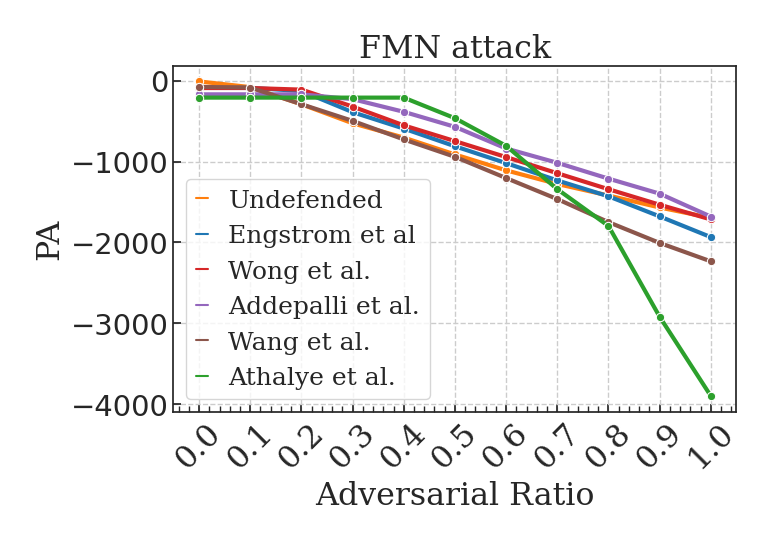
\includegraphics[width=\textwidth]{img/results_discussion/adversarial/FMN_logPA.png}
    \end{subfigure}
    \hfill
    \begin{subfigure}[b]{0.59\textwidth}
        \centering
        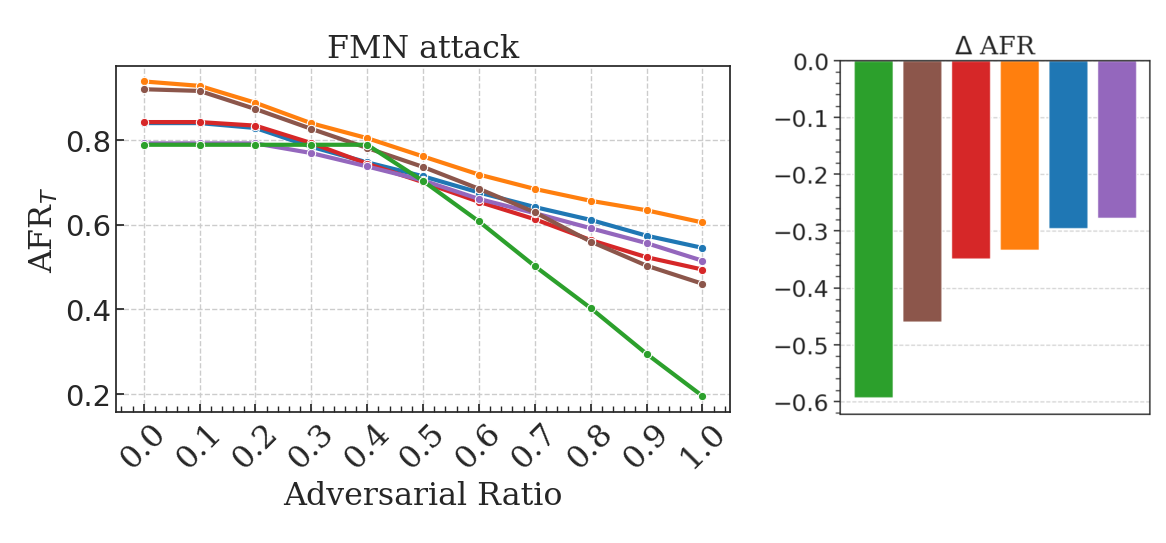
\includegraphics[width=\textwidth]{img/results_discussion/adversarial/FMN_1000_AFR_true.png}
    \end{subfigure}
    \caption{PA, $\operatorname{AFR}_\text{T}$ and the AFR variation against increasing adversarial ratio. 
    The aforementioned undefended net and several RobustBench robust models are considered 
    under a 1000 step FMN attack.}
    \label{fig:adv_fmn_pa_afr}
\end{figure}


As expected, the effectiveness of the FMN attack is superior to that of PGD attacks, as
the decrease in performance is substantially more significant for all models, especially the ones
previously considered robust. In this case, the assessment provided by PA is 

It is likely that these models have been defended with a
compression strategy that succeeds at filtering out small perturbations, which are
the ones employed by FMN, and for that reason maintain their performance at low
adversarial ratio values \cite{dasKeepingBadGuys2017}.
In particular, {\color{tab:green} \textbf{Athalye et al.}} remains maximally robust
until at least 40\% of the samples are perturbed, at which point the defensive strategy
is neutralized and a constant fraction of the additional perturbed samples succeeds at
misleading the model, which translates into a linear decrease in performance and PA. \\

PA proves to be very discriminative among robust models and to represent the 
phase transition entailed by the collapse of the defense strategy better than AFR does, which can be
observed in more detail in Figure \ref{fig:appendix_adversarial_afrpred_fmn}. A significative
result is that PA is not so directly aligned with $\Delta$AFR, in contrast to
the PGD case, which shows again that the decrease in performance is not the main driver of
the robustness assessment provided by PA, but instead can be interpreted as a consequence of
a misalignment in the posterior distributions of adversarial samples, which are the ones driving
the metric after the $\alpha$ thresold is reached. \\

\begin{figure}[H]
    \centering
    \begin{subfigure}[b]{\textwidth}
        \centering
        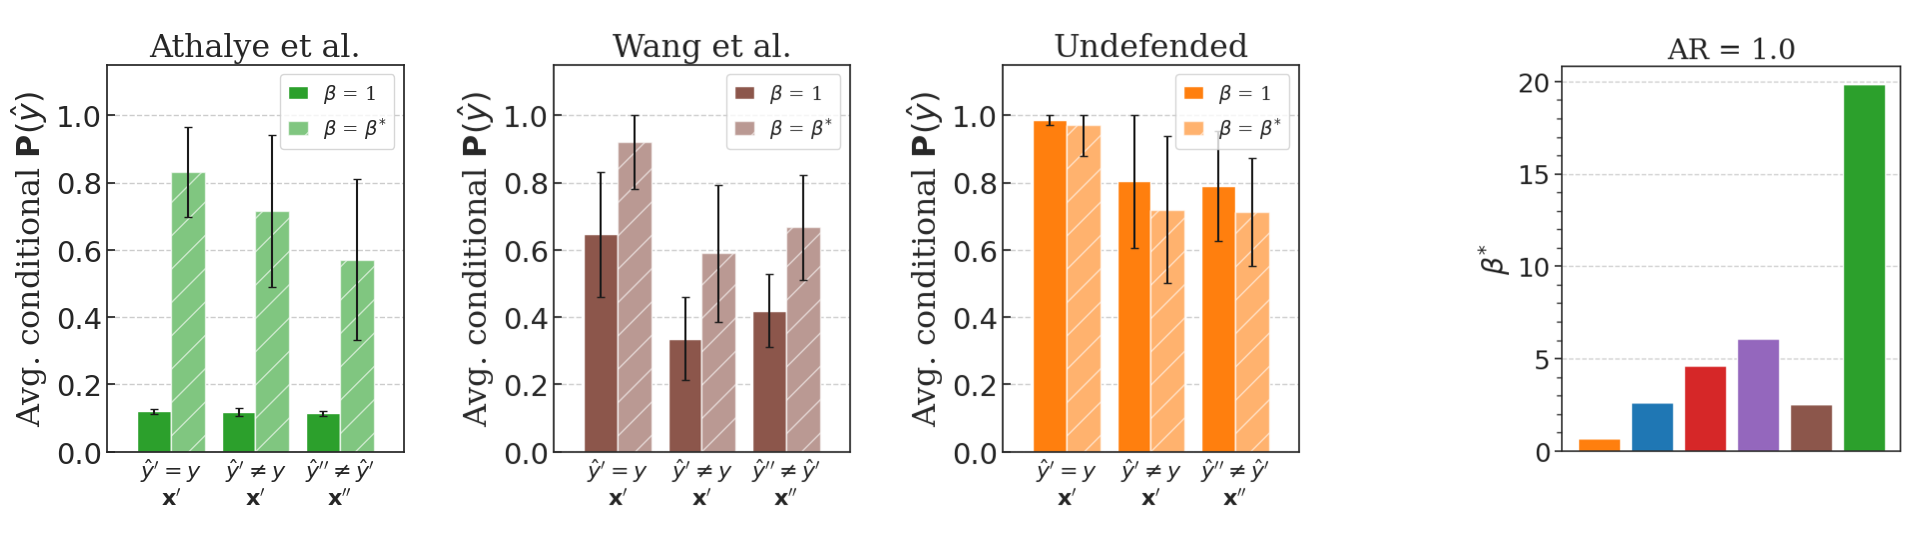
\includegraphics[width=\textwidth]{img/results_discussion/adversarial/bpda_wang_undefended_beta_fmn.png}
    \end{subfigure}
   
    \caption{(\textbf{left}) Average posterior probability of the predicted class for 
    correctly classified original samples, misclassified original samples, and 
    misleading adversarial samples, respectively. (\textbf{right}) Optimal $\beta^{*}$ value for each model.
    Results obtained through a FMN attack.}
    \label{fig:unrobust_posterior_short_fmn}
\end{figure}

Figure \ref{fig:unrobust_posterior_short_fmn} gives insight into the probabilistic output
of the model and the informativeness of the optimal posterior for the {\color{tab:orange} \textbf{Undefended}}, 
{\color{tab:green} \textbf{Athalye et al.}} and {\color{tab:brown} \textbf{Wang et al.}} models, in
analogous way to the PGD experiments. The first two models display a very similar behaviour for 
$\beta = 1$, but optimal posteriors are less informative due to the increased number of misleading
samples, which translates into a smaller $\beta^{*}$. The response of 
the {\color{tab:brown} \textbf{Wang et al.}} model further illustrates the higher effectiveness of
FMN attacks, as adversarial perturbations are on average more misleading than outlier samples in
the original dataset, which did not occur in the PGD case. Analogous representations for the remaining
models can be found in Figure \ref{fig:appendix_adversarial_distribution_fmn}, which show
that the {\color{tab:purple} \textbf{Addepalli et al.}} is the only robust model that maintains
the same behaviour under both attacks.\\

Overall, we recognize that PA has a higher discriminative power than AFR, especially
considering the evolution of each metric over increasing adversarial ratio, as
seen in Figures \ref{fig:six_figures_pa_adv} and \ref{fig:adv_fmn_pa_afr}. 
In particular, Figures \ref{fig:appendix_adversarial_afrpred_pgd} and \ref{fig:appendix_adversarial_afrpred_fmn}
compare the evolution of PA with that of AFR (P), which is the baseline metric for robustness,
and show the susceptibility of the latter to dataset variability. This is an important
consideration, as PA not only improves the discriminability in terms of the scale of
the differences between models, but also provides a more stable assessment across varying
levels of perturbed sample presence, under which AFR (P) exhibits significant fluctuations
that alter the ranking of the models at every step, as illustrated in Table \ref{tab:pa_afrpred_comparison_table}. \\

\begin{table}[h]
    \centering
    \resizebox{\textwidth}{!}{%
    \begin{tabular}{l|ccc|ccc|ccc}
    \multirow{2}{*}{} & \multicolumn{3}{c|}{$\alpha$ = 2/10} & \multicolumn{3}{c|}{$\alpha$ = 4/10} & \multicolumn{3}{c}{$\alpha$ = 6/10} \\
    % \cmidrule{2-10}
    \textbf{PGD} & PA & $\operatorname{AFR}_{\text{P}}$ & $\operatorname{AFR}_{\text{T}}$ & PA & $\operatorname{AFR}_{\text{P}}$  & $\operatorname{AFR}_{\text{T}}$ & PA & $\operatorname{AFR}_{\text{P}}$  & $\operatorname{AFR}_{\text{T}}$ \\
    \midrule
    {\color{tab:purple} \textbf{Addepalli et al.}} & \textbf{-172.5} & \textbf{0.995} & \textbf{0.785} & \textbf{-175.5} & 0.992  & \textbf{0.786} & \textbf{-177.6} & 0.989  & \textbf{0.783} \\
    {\color{tab:red} \textbf{Wong et al.}} & -97.7 & 0.996  & 0.838 & -102.9 & 0.992  & 0.834 & -109.2 & \textbf{0.987}  & 0.830 \\
    {\color{tab:blue} \textbf{Engstrom et al.}} & -94.2 & 0.996 & 0.836 & -104.6 & \textbf{0.990} & 0.830 & -110.3 & 0.988 & 0.829 \\
    {\color{tab:brown} \textbf{Wang et al.}} & -81.9 & 0.997 & 0.917 & -84.6 & 0.996 & 0.915 & -89.4 & 0.991 & 0.912 \\
    \midrule
    \addlinespace
    \addlinespace
    \textbf{FMN} & PA & $\operatorname{AFR}_{\text{P}}$ & $\operatorname{AFR}_{\text{T}}$ & PA & $\operatorname{AFR}_{\text{P}}$  & $\operatorname{AFR}_{\text{T}}$ & PA & $\operatorname{AFR}_{\text{P}}$  & $\operatorname{AFR}_{\text{T}}$ \\
    \midrule
    {\color{tab:purple} \textbf{Addepalli et al.}} & -169.4 & 1.0 & \textbf{0.791} & -385.4 & 0.944  & \textbf{0.737} & --838.9 & 0.867  & 0.660 \\
    {\color{tab:red} \textbf{Wong et al.}} & -111.2 & 0.991  & 0.834 & -553.1 & 0.901  & 0.743 & -944.8 & 0.810  & \textbf{0.653} \\
    {\color{tab:blue} \textbf{Engstrom et al.}} & -128.5 & 0.988 & 0.828 & -592.9 & 0.907 & 0.747 & -1020 & 0.836 & 0.675 \\
    {\color{tab:brown} \textbf{Wang et al.}} & \textbf{-291.6} & \textbf{0.952} & 0.873 & \textbf{-726.8} & \textbf{0.861} & 0.781 & \textbf{-1204} & \textbf{0.764} & 0.684 \\
    \bottomrule
    \end{tabular}%
    }
    \caption{
        Comparison of PA, $\operatorname{AFR}_{\text{P}}$ and $\operatorname{AFR}_{\text{T}}$ scores for a 
        PGD attack with $\ell_\infty$ = 16 / 255 and an FMN attack across different adversarial 
        ratio values. The worst robustness score is emboldened for every case.
        PA displays higher consistency and discriminative power 
        across varying $\alpha$ with respect to 
        accuracy-based metrics.
    }
    \label{tab:pa_afrpred_comparison_table}
\end{table}

\begin{table}[h]
    \centering
    \begin{tabular}{l|ccc|ccc}
    \multirow{2}{*}{} & \multicolumn{3}{c|}{$\alpha$ = 1/10} & \multicolumn{3}{c}{$\alpha$ = 5/10} \\
    % \cmidrule{2-10}
     & PA & $\operatorname{AFR}_{\text{P}}$ & $\operatorname{AFR}_{\text{T}}$ & PA & $\operatorname{AFR}_{\text{P}}$  & $\operatorname{AFR}_{\text{T}}$ \\
    \midrule
    PGD, $\ell_\infty$=8/255 & \textbf{1.0} & 0.0 & 0.66  & \textbf{1.0} & -0.66 & 0.66  \\  
    PGD, $\ell_\infty$=16/255 & \textbf{0.66} & -0.33 & 0.66 & 0.66  & \textbf{1.0} & 0.66 \\  
    PGD, $\ell_\infty$=32/255 & \textbf{0.66} & -0.33 & 0.66  & 0.66 & \textbf{1.0} & 0.66  \\  
    FMN & 0.33 & \textbf{0.66} & 0.0  & \textbf{1.0} & 1.0 & -0.66  \\  
    \bottomrule
    \end{tabular}
    \caption{
        Kendall rank correlation coefficient comparing the consistency of the model ranking
        provided by each metric at different adversarial ratio values. The raking at a specific $\alpha$ is 
        compared with that with $\alpha$ = 1.0. PA is shown to display the highest consistency, especially under
        low attack power settings.
    }
    \label{tab:kendall_comparison_table}
\end{table}

These observations lead to the conclusion that PA offers a more reliable
assessment of adversarial robustness, which in general aligns with the decrease
in performance on perturbed samples, but that relies heavily on the informativeness
of the posterior distribution and the confidence in the predictions for both
original and perturbed samples. \\

\subsection{Interpretability of PA in the adversarial setting}

In light of the results obtained, the suitability of
PA in the adversarial setting has been demonstrated, but a deeper exploration of the
reason of the discrepancies between PA and the baseline robustness measures is needed
so that it can confidently be established as a model selection criterion. In particular,
we will work with the approximated expression of PA derived in Theorem \ref{thm:approximated_pa} 
and ellucidate the source of the measured robust behaviour. \\

Table \ref{tab:approx_pa_pgd_table} shows the contribution of each subset of observations to the final
approximated PA value for a PGD attack. $N_{\text{ERR}}$, $N_{\text{MIS}}$ and $N_{\text{ADV}}$ are the number of (pairs of)
contributing samples, and $\Xi_{\text{ERR}}$, $\Xi_{\text{MIS}}$ and $\Xi_{\text{ADV}}$ are
the total amount of the contribution. For reasons described earlier in this section,
the PA approximation overestimates penalizations when compared to the true value, but
relative discrepancies between models are still largely preserved and therefore the rationale
behind the discriminative power of PA, as shown in Figures \ref{fig:appendix_adversarial_approx_pa_pgd}
and \ref{fig:appendix_adversarial_approx_pa_fmn}. The parameters $2 \delta_{\text{MIS}}$ and
$\delta_{\text{ADV}}$ account for the average probability assigned to classes other than the predicted
class for misclassified original samples and misleading adversarial samples, respectively, and 
help interpret the informativeness of the distibution as well as the value of each individual 
penalization. \\

For instance, a large $2 \delta_{\text{MIS}}$ value indicates robustness to sampling randomness, as it
represents higher average uncertainty in misclassified predictions. A model with a high performance on 
test data entails a more negative penalization $\log(1 - 2 \delta_{\text{MIS}})$, for being misclassified 
samples more likely to be equivalently misclassified under adversarial perturbations, but at
the same time makes misclassifications less likely, and therefore the number of terms added to
$\Xi_{\text{MIS}}$. The existing trade-off between standard and robust generalization arises when 
following this reasoning towards the minimization of $\Xi_{\text{MIS}}$, because reducing the number of 
misclassified samples will drive $\beta^{*}$ to higher values and therefore decrease adversarial 
uncertainty $\delta_{\text{ADV}}$. As outlined before, $\delta_{\text{ADV}}$ indicates 
robustness to adversarial perturbations, as it represents the average prediction uncertainty on adversarial 
misleading samples, and entails a penalization of $\log(\delta_{\text{ADV}})$. \\

The interpretation of these terms is vitally important for the purpose of this work, as it enables
the identification of the different sources of robustness displayed by each model, and therefore
the characterization of the randomness that we will demand models to generalize to. From a general 
perspective, $\Xi_{\text{SAM}} = \Xi_{\text{ERR}} + \Xi_{\text{MIS}}$ can be understood as the lack of robustness
to sampling randomness, and $\Xi_{\text{ADV}}$ as the lack of robustness to adversarial perturbations. \\


\begin{table}[H]
    \centering
    \begin{tabular}{l|rrr|rrr}
    Defense & $N_{\text{MIS}}$ & $2 \delta_{\text{MIS}}$ & $\Xi_{\text{SAM}}$ & $N_{\text{ADV}}$ & $\delta_{\text{ADV}}$ & $\Xi_{\text{ADV}}$ \\
    \midrule
    {\color{tab:brown} \textbf{Wang et al.}} & 799 & 0.24 & -468.62 & 47 & 0.44 & -39.44 \\
    {\color{tab:blue} \textbf{Engstrom et al.}} & 1591 & 0.17 & -566.72 & 67 & 0.39 & -63.43 \\
    {\color{tab:red} \textbf{Wong et al.}} & 1562 & 0.17 & -537.25 & 90 & 0.38 & -88.98 \\
    {\color{tab:purple} \textbf{Addepalli et al.}} & 2063 & 0.21 & -877.42 & 75 & 0.46 & -58.92 \\
    {\color{tab:orange} \textbf{Undefended}} & 566 & 0.47 & -736.63 & 810 & 0.24 & -1173.55 \\
    {\color{tab:green} \textbf{Athalye et al.}} & 1915 & 0.23 & -963.85 & 747 & 0.21 & -1183.96 \\
    \bottomrule
    \end{tabular}
    \caption{
    Approximated PA contributions for a PGD attack with $\ell_\infty$ = 8/255 and
    $\alpha = 1.0$. The number of originally misclassified and adversarially misleading
    samples is $N_{\text{MIS}} = \lfloor N (1-\operatorname{AFR}_T^0) \operatorname{AFR}_P \rfloor$ and
    $N_{\text{ADV}} = \lfloor N \operatorname{AFR}_T^0 (1-\operatorname{AFR}_P) \rfloor$, respectively. 
    The penalization argument $2 \delta_{\text{ERR}}$ has not
    been included for being negligible in all cases.
    }
    \label{tab:approx_pa_pgd_table}
\end{table}

As expected, the standard generalization error term $\Xi_{\text{SAM}}$ is the one contributing most to
the PA measure in robust models, as the selected PGD attack is not very effective and can only generate
a small number of misleading samples $N_{\text{ADV}}$. The discrimination of models based exclusively 
on $\Xi_{\text{SAM}}$  is very much aligned with that of $\operatorname{AFR}_\text{T}$ in all cases with the exception of the
{\color{tab:orange} \textbf{Undefended}} model, which is penalized more heavily for providing
overconfident predictions with a large number of misleading examples $N_{\text{ADV}}$ and
thus converging to a small $\beta^{*}$. This is an important realization, as it shows that even if
standard and adversarial robustness contributions can be dissociated, they are mutually dependent
and ultimately derive from the overall agreement in all predictions, regardless of the nature of the
randomness they are bound to. The generalization error to sampling randomness will be exceedigly penalized
the less robust a model is to other sources of randomness, because the optimal resolution of the hypothesis
space is reduced and the less distinction can be made between adversarial samples and outliers from
the original dataset. Further insights into this reasoning can be obtained by comparing these results
with those of the {\color{tab:green} \textbf{Athalye et al.}} model, which has a similar accuracy
on adversarial samples and a significantly worse accuracy on original samples. The fact that posterior
distributions are profoundly uninformative increases agreement in between mismatching posterior and
thus lowers penalization terms, even if more terms will be added as a consequence of the
associated decrease in performance. \\

The same reasoning can be followed to explain the discrimination made by PA between
{\color{tab:purple} \textbf{Addepalli et al.}} and the other robust models. {\color{tab:purple} \textbf{Addepalli et al.}}
experiences a comparable drop in performance, and for displaying a reduced confidence in mismatching predictions
is assigned a smaller $\Xi_{\text{SAM}}$ contribution than some of these models. Nevertheless, such 
uncertainty is also observed for original samples, which lowers accuracy on the original dataset 
and thus increases random sampling penalization $\Xi_{\text{SAM}}$. In that sense, it can be argued
that {\color{tab:purple} \textbf{Addepalli et al.}} is more robust than {\color{tab:red} \textbf{Wong et al.}}
and {\color{tab:blue} \textbf{Engstrom et al.}} to adversarial perturbations, which also stems from
the baseline AFR (P) and $\Delta$AFR values, but significantly less robust to sampling randomness.
PA weights both contributions and yields an intermediate model selection criterion. \\

Regarding adversarial robustness, we observe that $\Xi_{\text{ADV}}$ is driven by the decrase in 
performance under attack $\Delta$AFR, as $N_{\text{ADV}}$ penalization terms
are added. Nevertheless, the value of each of these terms is $\log(\delta_{\text{ADV}})$, which penalizes
models that achieve maximum posterior agreement by increasing confidence on adversarially
misleading examples. This is a clear distinctive trait with respect to accuracy-based metrics,
whose penalizations are reduced to a binary decision.


\begin{table}[H]
    \centering
    \begin{tabular}{l|rrr|rrr}
    Defense & $N_{\text{MIS}}$ & $2 \delta_{\text{MIS}}$ & $\Xi_{\text{SAM}}$ & $N_{\text{ADV}}$ & $\delta_{\text{ADV}}$ & $\Xi_{\text{ADV}}$ \\
    \midrule
    {\color{tab:purple} \textbf{Addepalli et al.}} & 1507 & 0.52 & -1910.69 & 2187 & 0.28 & -2788.89 \\
    {\color{tab:red} \textbf{Wong et al.}} & 1032 & 0.46 & -1125.53 & 2920 & 0.27 & -3844.40 \\
    {\color{tab:blue} \textbf{Engstrom et al.}} & 1125 & 0.72 & -2469.65 & 2505 & 0.32 & -2847.99 \\
    {\color{tab:brown} \textbf{Wang et al.}} & 435 & 0.82 & -1599.08 & 4215 & 0.33 & -4637.45 \\
    {\color{tab:orange} \textbf{Undefended}} & 412 & 0.56 & -704.58 & 3132 & 0.29 & -3906.55 \\
    {\color{tab:green} \textbf{Athalye et al.}} & 859 & 0.57 & -2054.23 & 4679 & 0.43 & -3955.43 \\
    \bottomrule
    \end{tabular}
    \caption{
    Approximated PA contributions for a FMN attack with $\alpha = 1.0$. The number of 
    originally misclassified and adversarially misleading
    samples is $N_{\text{MIS}} = \lfloor N (1-\operatorname{AFR}_T^0) \operatorname{AFR}_P \rfloor$ and
    $N_{\text{ADV}} = \lfloor N \operatorname{AFR}_T^0 (1-\operatorname{AFR}_P) \rfloor$, respectively. 
    The penalization argument $2 \delta_{\text{ERR}}$ has not
    been included for being negligible in all cases with the exception of the 
    {\color{tab:green} \textbf{Athalye et al.}} model, which amounts to 0.36. 
    }
    \label{tab:approx_pa_fmn_table}
    \end{table}

In contrast with the PGD case, the FMN attack is much more effective and $N_{\text{ADV}} > N_{\text{MIS}}$
in all cases, which makes the adversarial contribution $\Xi_{\text{ADV}}$ more relevant in the
overall robustness assessment. The discrepancy observed between PA and
accuracy-based metrics for the {\color{tab:red} \textbf{Wong et al.}} model can also be explained 
in these terms, as it is the least penalized by $\Xi_{\text{SAM}}$ among robust models due to its
superior accuracy. In the context of effective attacks, predictive certainty on
original samples is highly rewarded because lower overall agreement makes sampling penalization terms
$\log(1 - 2 \delta_{\text{MIS}})$ more negative. \\

Overall, this approximation shows that the final PA value stems from a combination of 
standard and adversarial generalization error, which are normally obtained independently through
different accuracy-based metrics, and leads to the realization that PA provides an intermediate
assessment in between AFR measures. An analogous combined metric weighting
accuracy and $\Delta$AFR would not be equiparable to PA, given that these weights would be arbitrary
and would not adjust to the particularities of each model. For instance, the 
{\color{tab:orange} \textbf{Undefended}} model should be mostly penalized on the basis of its
robustness to adversarial examples, whereas {\color{tab:purple} \textbf{Addepalli et al.}}
model should be mostly penalized for its lack of robustness to sampling randomness in the
original data. These considerations are fundamental in the covariate shift setting, as
different models with different defensive or invariant feature learning strategies will
navigate the generalization-complexity trade-off in a different way. \\

As a conclusion to our analysis, other kinds of metrics have been contrasted to determine whether they
are able to provide a reliable assessment of adversarial and sampling robustness that is comparable to
the baseline accuracy-based measures. These include confidence-based measurements,
such as the Kullback-Leibler (KL) divergence and the Wasserstein distance between posterior
distributions, and typical distance measures on the feature space of the model, namely 
through dataset cosine similarity, distance between centroids, and other cluster-based approaches 
such as the maximum mean discrepancy or the Fr\'{e}chet inception distance (FID). This last one is 
particularly interesting, as it is a widely used metric in the generative adversarial network 
literature and thus fits intuitively well into our setting. \\

\begin{figure}[H]
    \centering
    \begin{subfigure}[b]{0.3\textwidth}
        \centering
        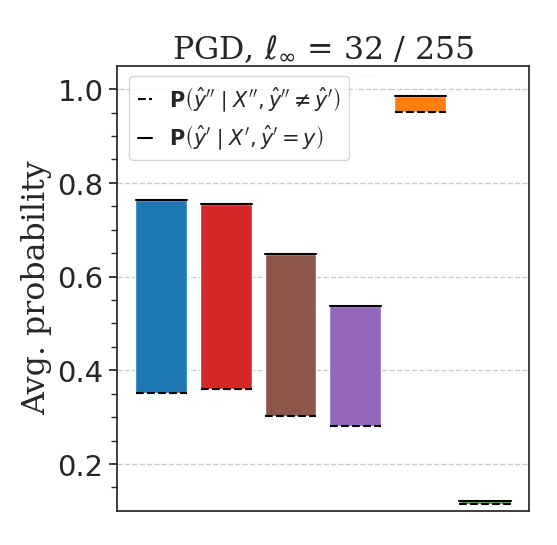
\includegraphics[width=\textwidth]{img/results_discussion/adversarial/DIFF_PGD_0.1255.png}
    \end{subfigure}
    \hfill
    \begin{subfigure}[b]{0.3\textwidth}
        \centering
        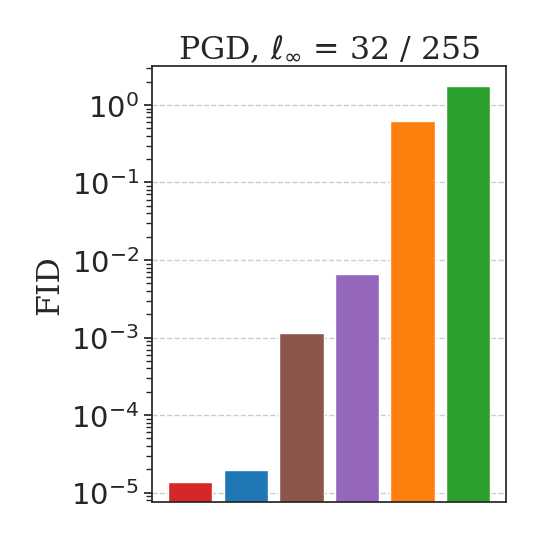
\includegraphics[width=\textwidth]{img/results_discussion/adversarial/FID_barplot_0.1255.png}
    \end{subfigure}
    \begin{subfigure}[b]{0.3\textwidth}
        \centering
        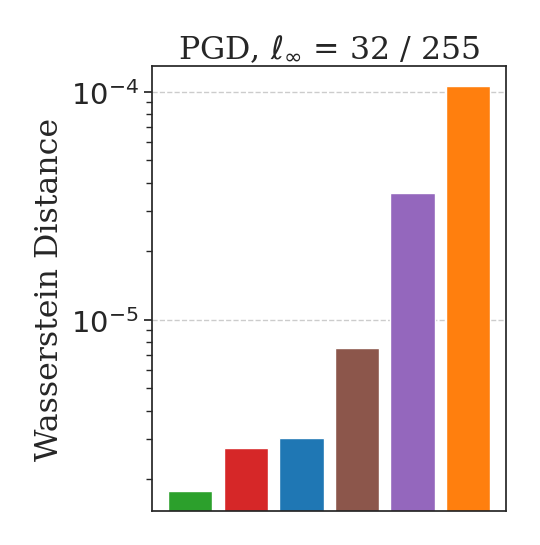
\includegraphics[width=\textwidth]{img/results_discussion/adversarial/W_barplot_0.1255.png}
    \end{subfigure}

    \vspace{1em}

    \begin{subfigure}[b]{0.3\textwidth}
        \centering
        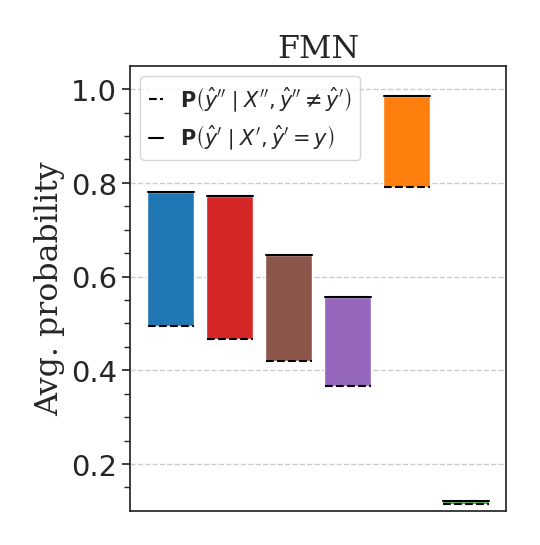
\includegraphics[width=\textwidth]{img/results_discussion/adversarial/DIFF_FMN.png}
    \end{subfigure}
    \hfill
    \begin{subfigure}[b]{0.3\textwidth}
        \centering
        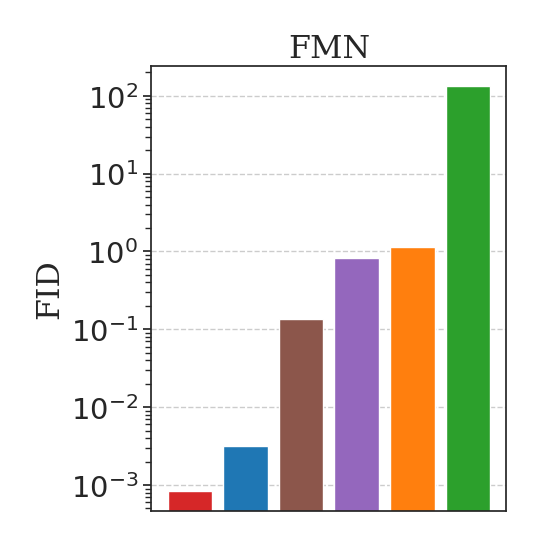
\includegraphics[width=\textwidth]{img/results_discussion/adversarial/FID_barplot_FMN.png}
    \end{subfigure}
    \begin{subfigure}[b]{0.3\textwidth}
        \centering
        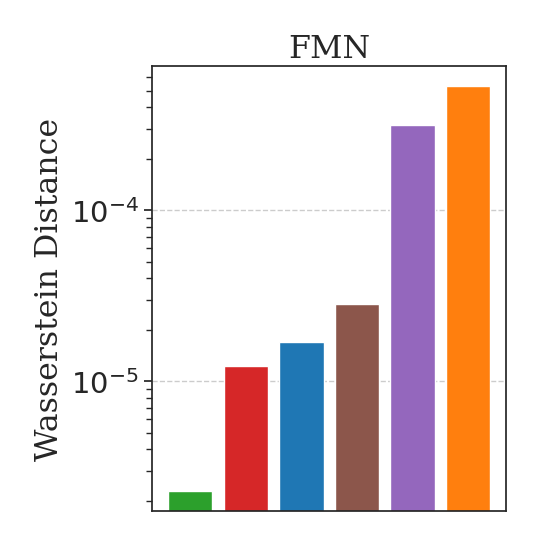
\includegraphics[width=\textwidth]{img/results_discussion/adversarial/W_barplot_FMN.png}
    \end{subfigure}

    \caption{
    The two metrics considered are FID, which amounts to the group-based dissimilarity 
    in the feature space, and Wasserstein distance, which measures the average distance between 
    probability distributions. 
    }
    \label{fig:adv_metric_comparison}
\end{figure}

Figure \ref{fig:adv_metric_comparison} displays some of these metrics for
PGD and FMN attacks, together with a condensed visualization of the average 
probability gap existing amidst predictions on original and adversarial examples. As
we can see, the discriminative power of these metrics stems from the overall difference 
between posteriors at $\beta = 1$. This result is not surprising, since the discriminant function 
of the classifier is constituted by a small subset of layers in the network, and is not expected 
to represent a complex discrimination that cannot be inferred from the distribution 
of samples in the feature space. As expected, probability-based metrics tend to concide in 
their assessment in general terms, and feature-space-based metrics as well. Besides, it is also not
surprising that feature space distances are more sensitive to the success rate of the attack, 
given that the inductive bias remains constant under any condition, whereas confidence-based metrics
are susceptible to the overall shift in the posterior, which in general favours non-informative
posteriors. A deeper insight into the evolution of these metrics for PGD and FMN attacks under increasing
adversarial ratio can be found in Figures \ref{fig:comparison_prob_metrics} and 
\ref{fig:comparison_feat_metrics}. \\

The results obtained in this section showcase the rationale behind the maximization of posterior
agreement, which can be thought of a surrogate version of the maximization of the mutual information
between original and perturbed datasets
\cite{buhmannDataScienceAlgorithms2022}. From an information-theoretic perspective, 
the maximization of mutual information effectively
distillates the information contained in the posterior distributions to that 
which is relevant for robustness assessment. This property is the source of the 
discriminative power displayed by PA and constitutes a fundamental difference
with respect to the baseline accuracy-based metrics considered.


\section{Out-of-distribution setting}\label{results_domain_generalization}

Following the analysis conducted in the previous section, the discriminability of PA
will be now explored in the domain generalization setting, which is a priori more convenient
for PA for being accuracy-based metrics less informative in this context. This is because
we are ultimately assessing the quality of the inductive bias of the model
by its ability to generalize to target (i.e. unseen) domains. In this sense, the additional
insight and discriminability exhibited by PA is expected to be more relevant for the selection of
models that perform well not only on unseen data, but also on unseen data that shares limited 
features with the training data. Under these conditions, the overlap between posteriors is more
informative than simply matching predictions (e.g. $\operatorname{AFR}_{\text{P}}$), because 
significant disagreement in
the remaining classes indicates vulnerability to distribution shifts present in
the source domains, which implies vulnerability to target domains as well. This is
a fundamental difference with respect to the adversarial setting, in which the nature of the
perturbation made posteriors less relevant for the robustness assessment.\\

This section will not address epoch-wise model selection, but will focus instead on 
the evaluation of the generalization capabilities of different learning algorithms under increasing 
levels of distribution shift, by computing the posterior agreement between source environments for 
models achieving maximum validation accuracy. More specifically, a baseline vanilla ERM algorithm will be 
used to train a ResNet18 model and will be compared with two robust 
learners, namely invariant risk minimization (IRM) and selective
augmentation (LISA), both introduced in Section \ref{sec:robust_learners}. Results should
ellucidate whether PA is able to discern datasets subjected to different levels of domain shift and
whether models achieving highest PA scores perform better on new domains. \\

Experiments will be performed by means of the DiagViB-6 dataset
framework
\cite{euligDiagViB6DiagnosticBenchmark2021}, 
which comprises MNIST images of size 128x128 within an augmentation pipeline enabling
the modification of six specific image factors: shape, hue, lightness, position,
scale and texture. Several variations in the \texttt{diagvibsix}
library\footnote{https://github.com/viictorjimenezzz/diagvibsix/tree/librarization}
have been implemented with the purpose 
of this project so that datasets can be built with a specific configuration of factors for each sample, which 
allows for a wide range of experiments in the data shift assessment and model selection settings. In
an analogous way to the adversarial case, datasets will be incrementally perturbed by including only
a fraction of the shifted samples, which in this context we will call shift ratio (SR).\\

Following the notation introduced in Section \ref{sec:domain_generalization_setting}, Definition 
\ref{def:shifted_factors_experiment} provides a characterization of source and target domains and
the randomness entailed by each dataset. The control over these aspects is the rationale behind
this experimental setup, since it is through synthetic image manipulation that we can maximize
invariant feature learning possibilities during training while providing optimal robustness
assessment conditions in validation and testing. Since changes in image factors can be independently 
introduced to each sample, the shifted dataset contains the same samples and in the same order
as the original dataset, thus removing sampling randomness contributions from the robustness score. 
Table \ref{tab:data_shift_table} stipulates the specific factors conforming each environment in this
experiment and Figure \ref{fig:data_shift_images} illustrates them with some examples.

CITE MORE INFO IN \ref{def:diagvib6_experiments} \\

\begin{definition}[Shifted factors experiment]\label{def:shifted_factors_experiment}
    The classification task involves the prediction of the shape factor (i.e. the digit)
    of handwritten fours and nines from the MNIST dataset. In particular, source and target
    domains are generated as follows:

    $$
    \begin{aligned}
        &\mathcal{S} = \{ X_0, X_1\},\\
        &\mathcal{T} = \{ X_1, X_2, X_3, X_4, X_5\},
    \end{aligned}
    $$

    where $X_j$ represents the random variable associated to domain $j$, 
    being $j$ the number of shifted factors with respect to domain $X_0$. 
    Datasets are generated by considering
    four different realizations of the experiment, namely $\tau_0^{\text{train}}$, $\tau_1^{\text{train}}$, $\tau^{\text{val}}$
    and $\tau^{\text{test}}$, each sampling from disjoint subsets of MNIST. Following the notation introduced
    in Chapter \ref{sec:experimental_setup}, we can define:
    $$
    \begin{aligned}
        &D^{\text{train}} = \{\bm{x}_0^{\text{train}}, \bm{x}_1^{\text{train}}\}, \; \text{where } \bm{x}_j := \bm{x}_j \circ \tau_j^{\text{train}}, \;j = 0,1 \\
        &D^{\text{val}} = \{\bm{x}_0^{\text{val}}, \bm{x}_1^{\text{val}}\}, \; \text{where } \bm{x}_j := \bm{x}_j \circ \tau^{\text{val}}, \;j=0,1 \\
        &D_j^{\text{test}} = \{\bm{x}_j^{\text{test}}\}, \; \text{where } \bm{x}_j^{\text{test}} := \bm{x}_j^{\text{test}} \circ \tau^{\text{test}}, \;j = 1,\dots,5
    \end{aligned}
    $$

    In this way, only training data is subject to both sampling randomness ($\tau_0^{\text{train}} \neq \tau_1^{\text{train}}$)
    and domain shift ($X_0 \nsim X_1$), emulating the conditions of real-world sampling experiments.
    In contrast, validation and testing datasets entail each a single noise instantiation, 
    which means that distribution shift is the only accountable source of randomness.
    Overall, two sets of $40\,000$ images for training, two sets of $20\,000$ 
    images for validation, and six sets of $10\,000$ images for testing are generated. 
\end{definition}

\begin{table}[H]
    \centering
    \begin{tabular}{l|c|c|c|c|c|c}
    \# Shift Factors & 0 & 1 & 2 & 3 & 4 & 5 \\
    \midrule
    Hue & red & \textbf{blue} & blue & blue & blue & blue \\
    Lightness & dark & dark & \textbf{bright} & bright & bright & bright \\
    Position  & CC & CC & CC & \textbf{LC} & LC & LC \\
    Scale  & normal & normal & normal & normal & \textbf{large} & large \\
    Texture & blank & blank & blank & blank & blank & \textbf{tiles} \\
    \textit{Shape} & \textit{4,9} &  \textit{4,9} &  \textit{4,9} & \textit{4,9} & \textit{4,9} & \textit{4,9} \\
    \bottomrule
    \end{tabular}
    \caption{
    Image factors associated to each of the environments considered in this experiment. CC and LC account
    for 'centered center' and 'centered low', respectively.
    }
    \label{tab:data_shift_table}
\end{table}


\begin{figure}[H]
    \centering
    \begin{subfigure}[b]{0.2\textwidth}
        \centering
        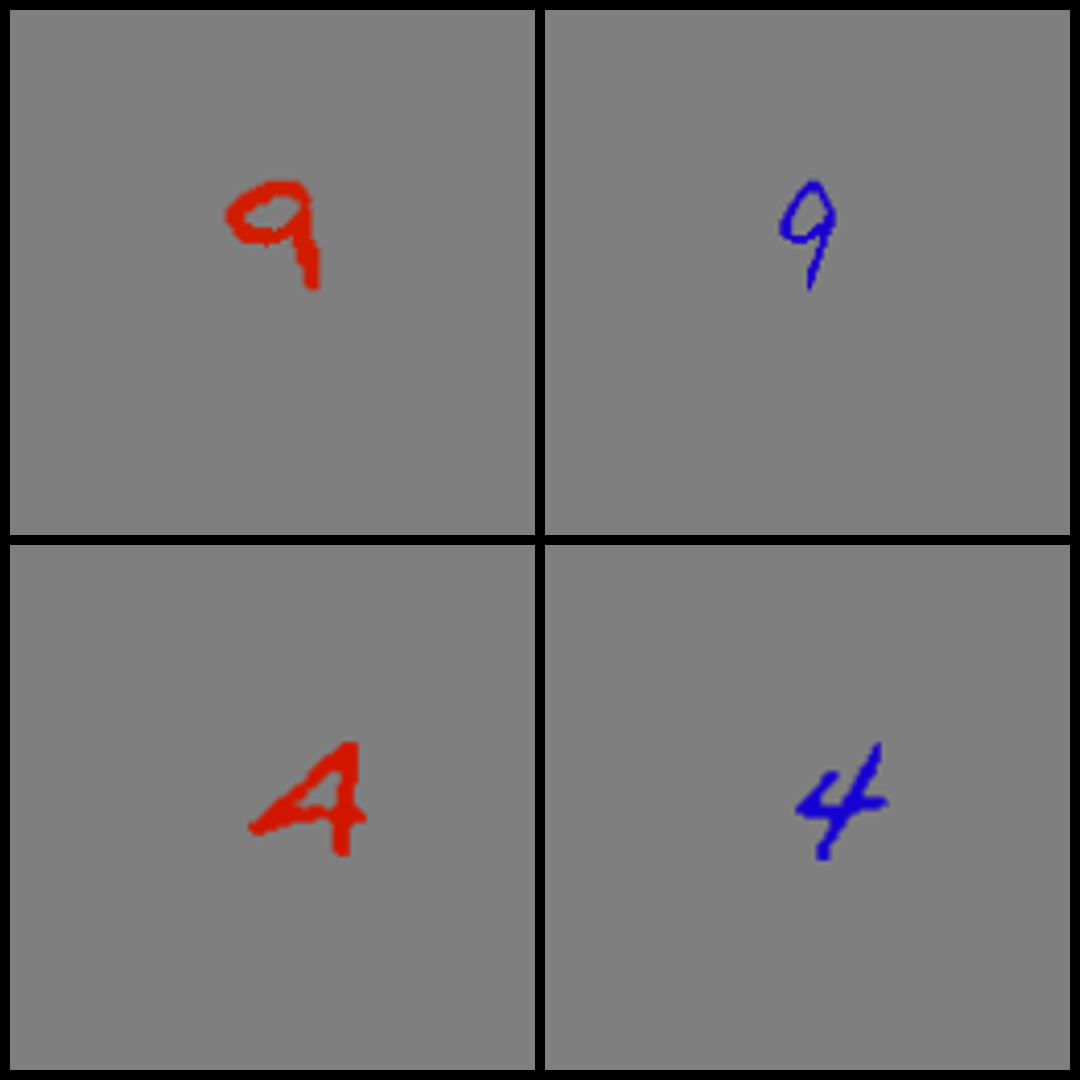
\includegraphics[height=2cm]{img/results_discussion/datashift/dsimages/train_collage.png}
        \caption*{Train}
    \end{subfigure}%
    \hfill
    \begin{subfigure}[b]{0.2\textwidth}
        \centering
        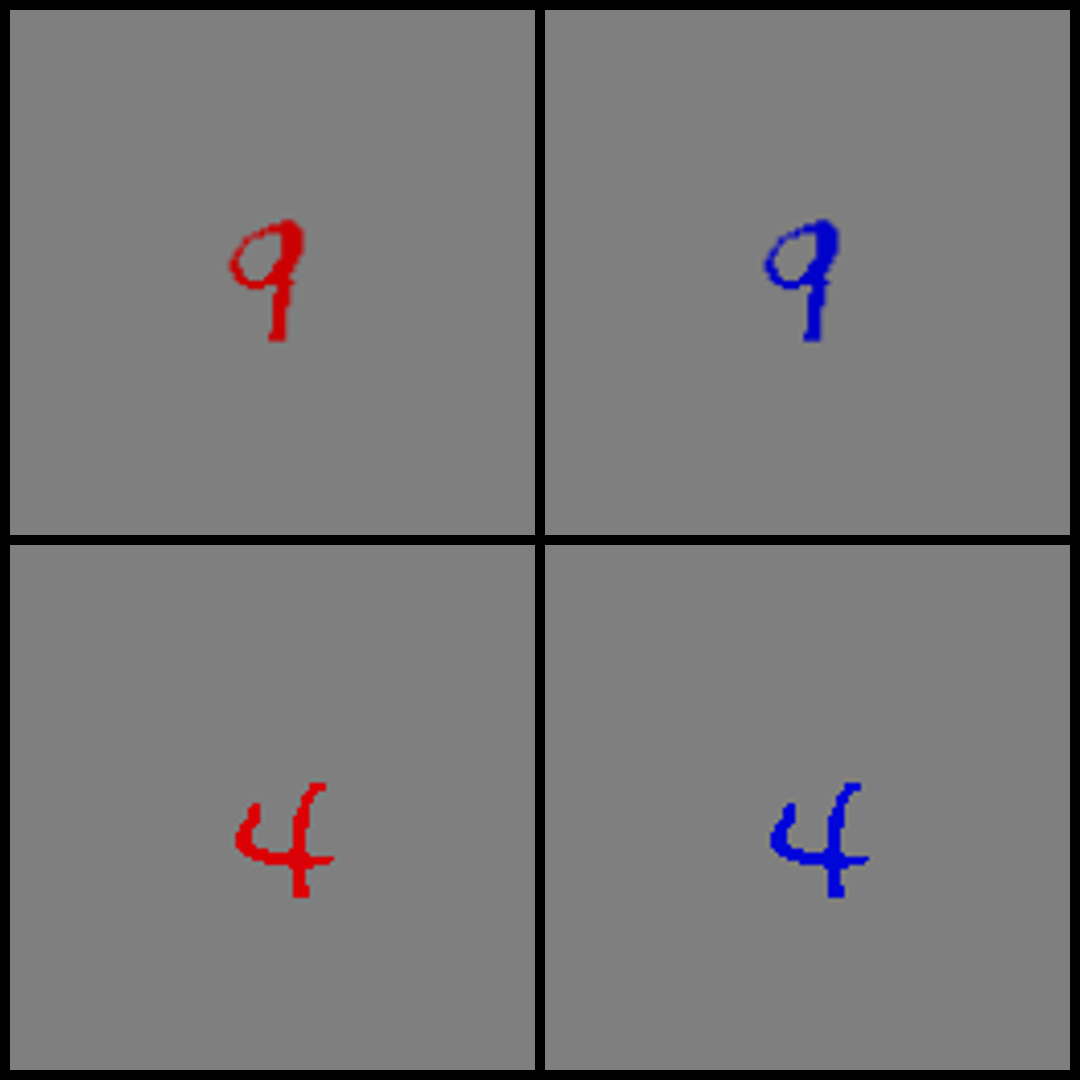
\includegraphics[height=2cm]{img/results_discussion/datashift/dsimages/val_collage.png}
        \caption*{Validation}
    \end{subfigure}%
    \hfill
    \begin{subfigure}[b]{0.6\textwidth}
        \centering
        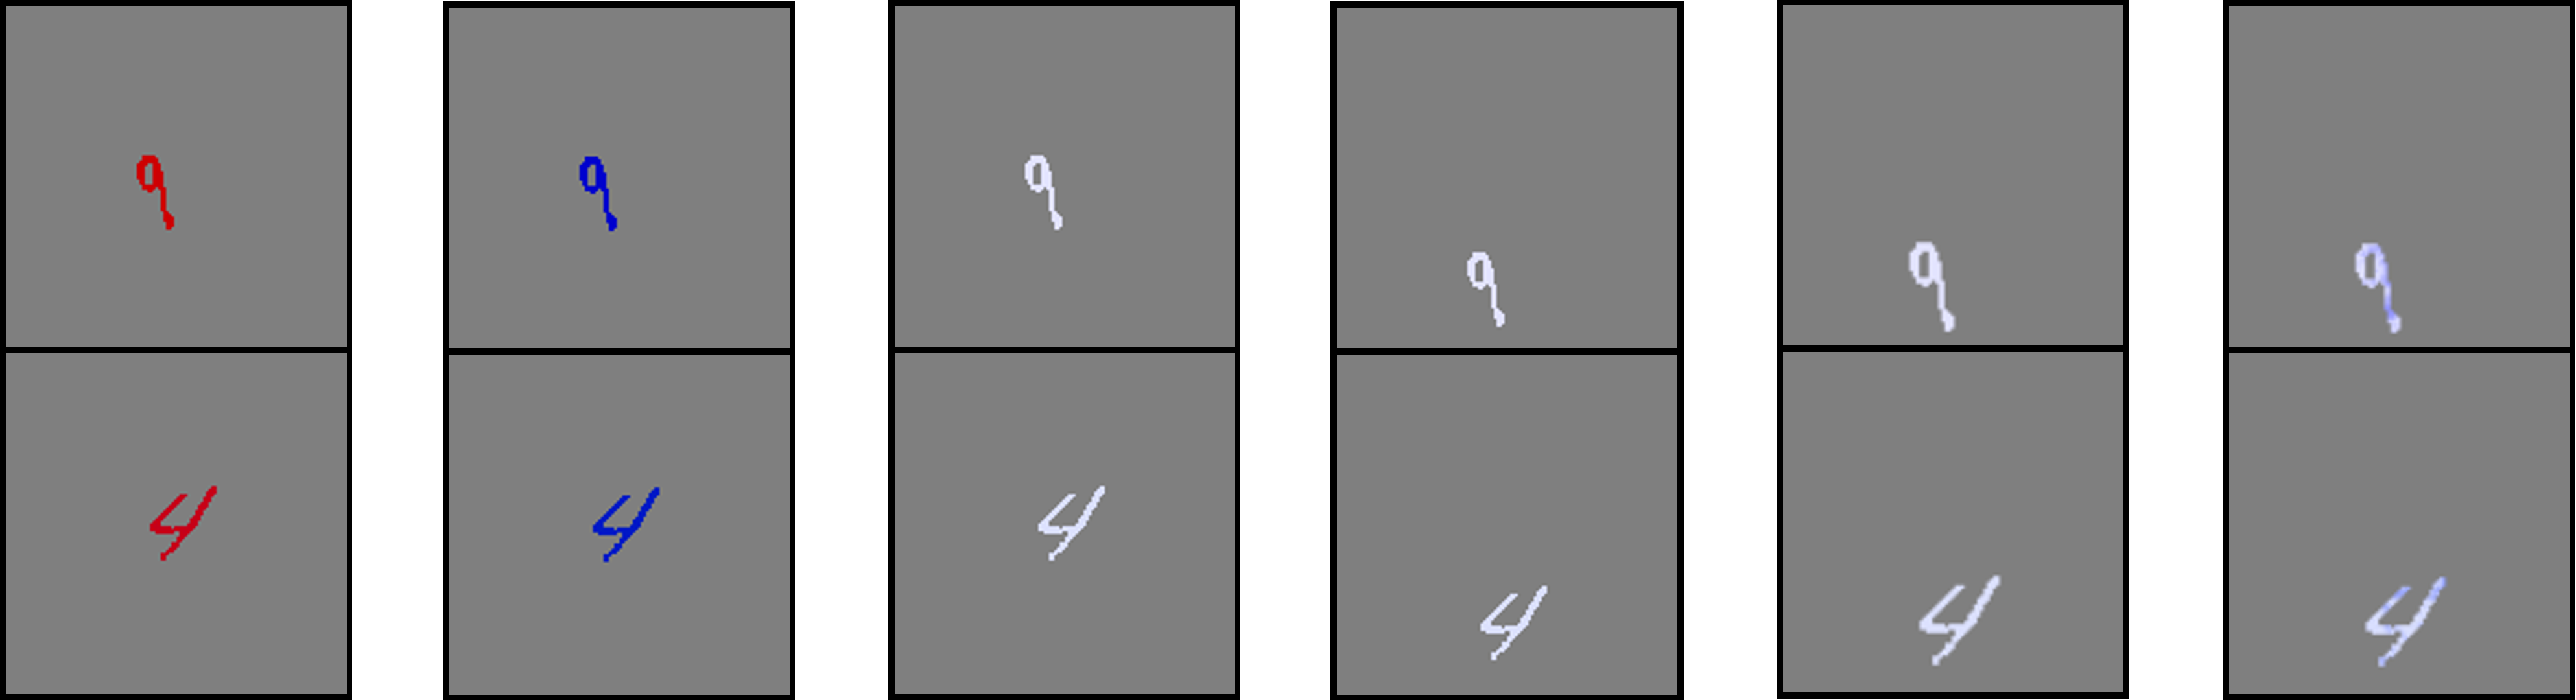
\includegraphics[height=2cm]{img/results_discussion/datashift/dsimages/test_collage2.png}
        \caption*{Test (1 - 5)}
    \end{subfigure}
    \caption{
    Illustration of the training, validation and test datasets. Samples for each
    training environment belong to different MNIST subsets, whereas samples of
    validation and test are corresponding.
    }
    \label{fig:data_shift_images}
\end{figure}


Results obtained in this setup show that PA succeeds at discriminating the 
different models by their predictive response under increasing number of shifted samples and 
under increasing shift power. In particular, ERM can be identified to be non-robust by the fact 
that its score is maximum for the first shifted factor, but decays rapidly to the minimum value 
after the second factor. In contrast, IRM and LISA show a reduced rate of decay and even display a
slight increase in performance for the last shift factor. \\

\begin{figure}[H]
    \centering
    \begin{subfigure}[b]{0.3\textwidth}
        \centering
        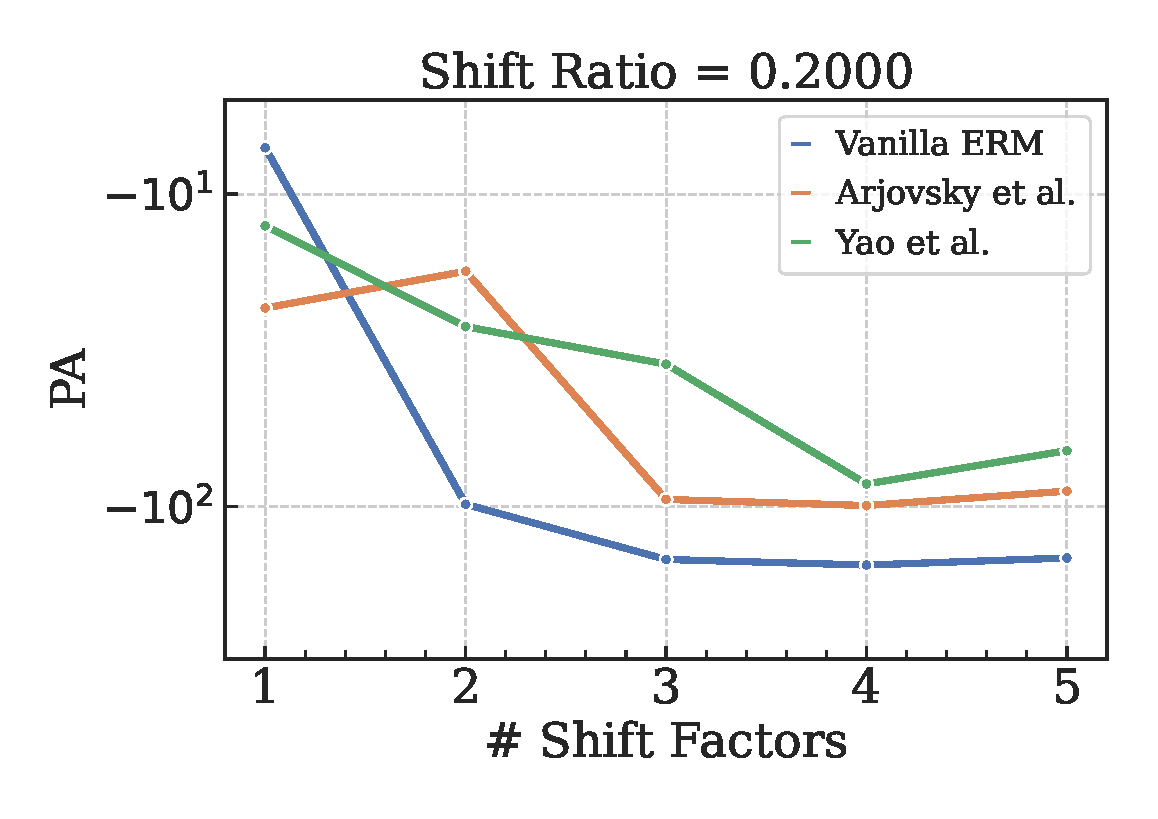
\includegraphics[width=\textwidth]{img/results_discussion/datashift/shift_ratio=0.200.pdf}
    \end{subfigure}
    \hfill
    \begin{subfigure}[b]{0.3\textwidth}
        \centering
        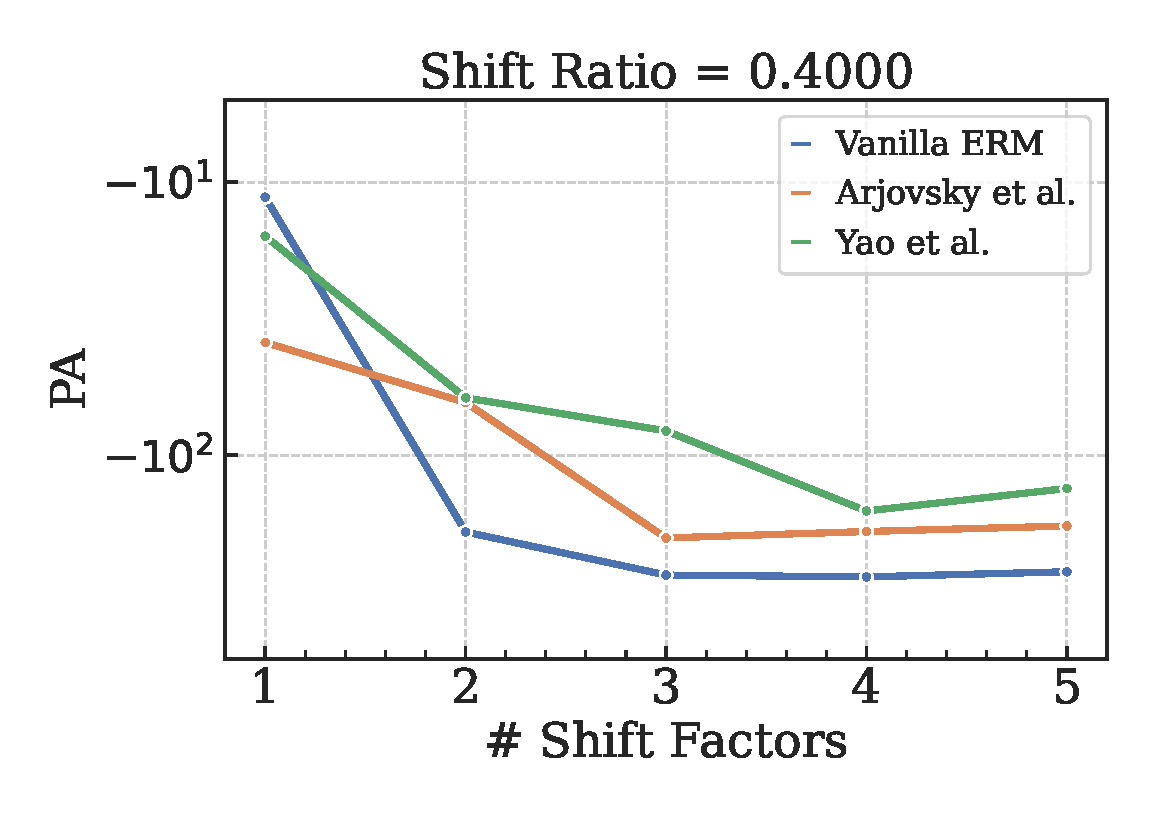
\includegraphics[width=\textwidth]{img/results_discussion/datashift/shift_ratio=0.400.pdf}
    \end{subfigure}
    \hfill
    \begin{subfigure}[b]{0.3\textwidth}
        \centering
        \includegraphics[width=\textwidth]{img/results_discussion/datashift/shift_ratio=0.600.pdf}
    \end{subfigure}

    \vspace{1em}

    \begin{subfigure}[b]{0.3\textwidth}
        \centering
        \includegraphics[width=\textwidth]{img/results_discussion/datashift/shift_ratio=0.800.pdf}
    \end{subfigure}
    \hspace{13pt}
    \begin{subfigure}[b]{0.3\textwidth}
        \centering
        \includegraphics[width=\textwidth]{img/results_discussion/datashift/shift_ratio=1.000.pdf}
    \end{subfigure}

    \caption{Evolution of PA under increasing levels of shift power. Weights maximizing validation
    accuracy were selected for ERM, IRM and LISA algorithms. Results for incremental presence of shifted
    samples indicate that PA is able to differentiate weak and robust models.
    }
    \label{fig:six_figures}
\end{figure}

The unexpected increase in PA after four shifted factors seems
inconsistent with the alleged non-increasing behaviour of PA, as per
Section \ref{sec:robustness_to_covariate_shift}. Nevertheless, this phenomenon 
only highlights that robustness does not stem from the data generation process but instead 
from the latent representation of the model and the features selected for the construction 
of its inductive bias, as discussed in the introductive chapter. In this particular case, 
Table \ref{tab:CS_shift} shows that
there is a clear discontinuity in the feature representation of the data when the texture
factor is shifted, which results in a different discriminator function that ultimately
leads to a predictive behaviour that aligns slightly better with the original predictions. \\

\begin{table}[H]
    \centering
    \begin{tabular}{l|c|c|c|c|c}
    \# Shift Factors & 1 & 2 & 3 & 4 & 5 \\
    \midrule
    {\color{tab:blue} \textbf{Vanilla ERM}} & 0.9978 & 0.9303 & 0.9562 & 0.9561 & \textbf{0.6661} \\
    {\color{tab:orange} \textbf{Arjovsky et al.}} & 0.9967 & 0.9018 & 0.9296 & 0.9374 & \textbf{0.5585} \\
    {\color{tab:green} \textbf{Yao et al.}}  & 0.9980 & 0.9431 & 0.9431 & 0.9641 & \textbf{0.7130} \\
    \bottomrule
    \end{tabular}
    \caption{
    Pairwise cosine similarity between feature space representations of original and
    augmented images, for each of the shifted datasets. The abrupt decrease in similarity
    for the fifth environment indicates a discontinuity in the feature representation of images,
    which leads to non-comparable predictive outcomes.
    }
    \label{tab:CS_shift}
    \end{table}


% - Here explain that PA can also be approximated by considering $\beta$ a fixed beta and evaluating
% in many environments. This validity of this approximation will be higher the lower is the decrease
% in performance of the model under increasing shift power. In any case, the assessment won't be optimal
% but can be used to spare computational ressources. Figure \ref{fig:datashift_eval_pa} shows the evaluated PA (i.e. $\beta^{*}$ computed only for the
% first two environments) for each model against the standard accuracy displayed during the whole
% optimization process. \\


% \begin{figure}[H]
%     \centering
%     \begin{subfigure}[b]{0.45\textwidth}
%         \centering
%         \includegraphics[width=\textwidth]{img/results_discussion/datashift/paper_oracle_all_erm.png}
%     \end{subfigure}
%     \hfill
%     \begin{subfigure}[b]{0.45\textwidth}
%         \centering
%         \includegraphics[width=\textwidth]{img/results_discussion/datashift/paper_PA_all_erm.png}
%     \end{subfigure}

%     \vspace{1em}

%     \begin{subfigure}[b]{0.45\textwidth}
%         \centering
%         \includegraphics[width=\textwidth]{img/results_discussion/datashift/paper_oracle_all_irm.png}
%     \end{subfigure}
%     \hfill
%     \begin{subfigure}[b]{0.45\textwidth}
%         \centering
%         \includegraphics[width=\textwidth]{img/results_discussion/datashift/paper_PA_all_irm.png}
%     \end{subfigure}

%     \caption{PA evaluation.}
%     \label{fig:datashift_eval_pa}
% \end{figure}

% \begin{figure}
%     \centering
%     \includegraphics[width=0.7\textwidth]{img/results_discussion/datashift/model_selection.png}
%     \caption{Model selection capabilities.}
%     \label{fig:model_selection_capabilities}
% \end{figure}



\begin{table}[h]
    \centering
    \resizebox{\textwidth}{!}{%
    \begin{tabular}{l|ccc|ccc|ccc}
    \multirow{2}{*}{} & \multicolumn{3}{c|}{1 Shifted Factor} & \multicolumn{3}{c|}{3 Shifted Factors} & \multicolumn{3}{c}{5 Shifted Factors} \\
     & PA & $\operatorname{AFR}_{\text{P}}$ & $\operatorname{AFR}_{\text{T}}$ & PA & $\operatorname{AFR}_{\text{P}}$  & $\operatorname{AFR}_{\text{T}}$ & PA & $\operatorname{AFR}_{\text{P}}$  & $\operatorname{AFR}_{\text{T}}$ \\
    \midrule
    {\color{tab:blue} \textbf{Vanilla ERM}} & \textbf{-24.91}  & 0.999 & 0.993 & -625.6 & 0.979 & 0.975 & -579.38 & 0.976 & 0.873 \\
    {\color{tab:orange} \textbf{Arjovsky et al.}} & -76.76 & 0.998 & 0.993 & -514.2 & 0.976 & 0.978  & -464.2 & 0.976 & 0.911 \\
    {\color{tab:green} \textbf{Yao et al.}} & -26.21 & \textbf{0.999} & \textbf{0.994} & \textbf{-201.2} & \textbf{0.985} & \textbf{0.980} & \textbf{-324.4} & \textbf{0.988} & \textbf{0.945} \\
    \bottomrule
    \end{tabular}
    }
    \caption{
        Comparison of PA, $\operatorname{AFR}_{\text{P}}$ and $\operatorname{AFR}_{\text{T}}$ scores
        for ERM, IRM and LISA learning algorithms under different levels of shift power. The highest robustness 
        score is emboldened for every case. PA is able to discriminate algorithms consistently and distinguish
        the first shifted factor, which is seen by the model during training, from the rest.
    }
    \label{tab:shift_comparison_table}
\end{table}

% As shown in Figure \ref{fig:datashift_selection}, PA-based model selection behaves differently in robust
% and non-robust algorithms. Following the reasoning derived in previous sections, it is likely that the PA
% assessment on ERM is mostly driven by standard generalization error, due to the fact that ERM is agnostic
% of the environment to which each sample belongs to and therefore to the accountable source of randomness represented
% by the environment shift. The risk minimization problem under these conditions should give rise to less informative
% predictive outcomes, given that the domain-invariant features associated with the task are less accessible, and
% thus reduce the penalization weight of mismatching samples. This intuition is supported by the fact that ERM
% optimization yields models that performs worse in all test datasets than the ones obtained through IRM,
% as can be seen in Figure \ref{fig:datashift_eval_pa}. Besides, results show that the selected model for ERM 
% performs better an all metrics for the first test environment, which contains
% the same factor configuration as one of the validation environments, and maintains or slightly decreases its performance
% for increasing levels of shift. In addition, the PA-selected model appears to encode a slight variation of the 
% decision rule from that of the accuracy-selected model, given that samples near to the decision boundary are now
% more likely classified as nines than fours, which increases specificity as much as it decreases sensitivity. \\

% Regarding PA-based model selection in robust learners, we observe the opposite behaviour. Since models are more likely
% to represent domain-invariant features, each with its distinctive strategy, predictive outcomes are expected to
% be more informative and thus increase the penalization contribution of mismatching samples, which will be the ones
% containing domain-invariant features that are not sufficiently considered in the inductive bias of the model. PA
% model selection under these conditions is thus more likely to favor sets of weights that perform better under
% increasing levels of shift, at the expense of losing predictive power on the environments in which it operated. 
% Results align with this interpretation, as we observe a notable increase in performance across all shifted datasets
% with respect to the accuracy-selected model, especially in the LISA case, at the expense of significantly decreasing
% performance on the first environment.\\


% \begin{figure}[H]
%     \centering
%     \begin{subfigure}[b]{0.6\textwidth}
%         \centering
%         \includegraphics[width=\textwidth]{img/results_discussion/datashift/paper_selection_ppred=1.0_met=acc.png}
%     \end{subfigure}

%     \begin{subfigure}[b]{0.6\textwidth}
%         \centering
%         \includegraphics[width=\textwidth]{img/results_discussion/datashift/paper_selection_ppred=1.0_met=sensitivity.png}
%     \end{subfigure}

%     \begin{subfigure}[b]{0.6\textwidth}
%         \centering
%         \includegraphics[width=\textwidth]{img/results_discussion/datashift/paper_selection_ppred=1.0_met=specificity.png}
%     \end{subfigure}
%     \caption{
%     Accuracy, sensitivity and precision displayed by sets of ResNet18 weights on
%     shifted test datasets, obtained through ERM, IRM and LISA
%     training procedures. Accuracy-based selection is compared to PA-based selection, both
%     operating with a validation dataset composed of samples of environments 0 and 1.
%     }
%     \label{fig:datashift_selection}
% \end{figure}



% Model:  0
% Accuracy:  [88.08000088 97.94499874 98.05499911 97.94499874 99.44000244]
% PA_diff:  [ 6.52999878e+00 -5.00082970e-03 -3.19999456e-01 -1.19996071e-01
%  -7.50005245e-02]
% Model:  1
% Accuracy:  [89.34500217 98.00500274 97.43499756 97.11999893 99.36000109]
% PA_diff:  [-6.13500476  0.          0.41000247  0.88000298  0.01499653]
% Model:  2
% Accuracy:  [89.74499702 95.35499811 95.3700006  95.59500217 99.32000041]
% PA_diff:  [-4.24499512  1.85500383  1.87000036  1.78999901  0.06999969]



% \begin{table}[H]
%     \centering
%     \resizebox{\textwidth}{!}{%
%     \begin{tabular}{l|cl|cl|cl|cl|cl|cl}
%     \multirow{2}{*}{} & \multicolumn{2}{c|}{\textbf{0}} & \multicolumn{2}{c|}{\textbf{1}} & \multicolumn{2}{c|}{\textbf{2}} & \multicolumn{2}{c|}{\textbf{3}} & \multicolumn{2}{c|}{\textbf{4}} & \multicolumn{2}{c}{\textbf{5}} \\
%     \textbf{{\color{tab:blue} \textbf{ERM}}} & Acc. & $\Delta_{\operatorname{PA}}$ & Acc. & $\Delta_{\operatorname{PA}}$ & Acc. & $\Delta_{\operatorname{PA}}$ & Acc. & $\Delta_{\operatorname{PA}}$ & Acc. & $\Delta_{\operatorname{PA}}$ & Acc. & $\Delta_{\operatorname{PA}}$ \\
%     \midrule
%     Specificity & 99.4 & \PlusMinus 0.01 & 68.0 & {\color{tab:green}  \textbf{\Plus 10.1}} & 45.2 & {\color{tab:red} \textbf{\Minus 10.1}} & 42.1 & {\color{tab:red} \textbf{\Minus 6.0}} & 42.9 & {\color{tab:red} \textbf{\Minus 9.3}} & 32.0 & {\color{tab:red} \textbf{\Minus 3.8}} \\
%     Sensitivity & \textbf{99.4} & \PlusMinus 0.01 & 67.1 & {\color{tab:red} \textbf{\Minus 7.9}} & 44.9 & {\color{tab:green}  \textbf{\Plus 0.8}} & 42.7 & {\color{tab:green}  \textbf{\Plus 1.3}} & 39.1 & {\color{tab:green}  \textbf{\Plus 1.5}} & 30.3 & {\color{tab:green}  \textbf{\Plus 1.4}} \\
%     \midrule
%     Accuracy & 88.1 & \PlusMinus 0.01 & 97.9 & \PlusMinus 0.01 & 98.1 & \PlusMinus 0.01 & 97.9 & \PlusMinus 0.01 & 42.5 & \PlusMinus 0.01 & 32.8 & \PlusMinus 0.01 \\
%     \midrule
%     \addlinespace
%     \addlinespace
%     \textbf{{\color{tab:orange} \textbf{IRM}}} & Acc. & $\Delta_{\operatorname{PA}}$ & Acc. & $\Delta_{\operatorname{PA}}$ & Acc. & $\Delta_{\operatorname{PA}}$ & Acc. & $\Delta_{\operatorname{PA}}$ & Acc. & $\Delta_{\operatorname{PA}}$ & Acc. & $\Delta_{\operatorname{PA}}$ \\
%     \midrule
%     Specificity & 99.4 & \PlusMinus 0.01 & 68.0 & {\color{tab:green}  \textbf{\Plus 10.1}} & 45.2 & {\color{tab:red} \textbf{\Minus 10.1}} & 42.1 & {\color{tab:red} \textbf{\Minus 6.0}} & 42.9 & {\color{tab:red} \textbf{\Minus 9.3}} & 32.0 & {\color{tab:red} \textbf{\Minus 3.8}} \\
%     Sensitivity & \textbf{99.4} & \PlusMinus 0.01 & 67.1 & {\color{tab:red} \textbf{\Minus 7.9}} & 44.9 & {\color{tab:green}  \textbf{\Plus 0.8}} & 42.7 & {\color{tab:green}  \textbf{\Plus 1.3}} & 39.1 & {\color{tab:green}  \textbf{\Plus 1.5}} & 30.3 & {\color{tab:green}  \textbf{\Plus 1.4}} \\
%     \midrule
%     Accuracy & 99.4 & \PlusMinus 0.01 & 59.3 & \PlusMinus 0.01 & 46.7 & \PlusMinus 0.01 & 44.9 & \PlusMinus 0.01 & 42.5 & \PlusMinus 0.01 & 32.8 & \PlusMinus 0.01 \\
%     \midrule
%     \addlinespace
%     \addlinespace
%     \textbf{{\color{tab:green} \textbf{LISA}}} & Acc. & $\Delta_{\operatorname{PA}}$ & Acc. & $\Delta_{\operatorname{PA}}$ & Acc. & $\Delta_{\operatorname{PA}}$ & Acc. & $\Delta_{\operatorname{PA}}$ & Acc. & $\Delta_{\operatorname{PA}}$ & Acc. & $\Delta_{\operatorname{PA}}$ \\
%     \midrule
%     Specificity & 99.4 & \PlusMinus 0.01 & 68.0 & {\color{tab:green}  \textbf{\Plus 10.1}} & 45.2 & {\color{tab:red} \textbf{\Minus 10.1}} & 42.1 & {\color{tab:red} \textbf{\Minus 6.0}} & 42.9 & {\color{tab:red} \textbf{\Minus 9.3}} & 32.0 & {\color{tab:red} \textbf{\Minus 3.8}} \\
%     Sensitivity & \textbf{99.4} & \PlusMinus 0.01 & 67.1 & {\color{tab:red} \textbf{\Minus 7.9}} & 44.9 & {\color{tab:green}  \textbf{\Plus 0.8}} & 42.7 & {\color{tab:green}  \textbf{\Plus 1.3}} & 39.1 & {\color{tab:green}  \textbf{\Plus 1.5}} & 30.3 & {\color{tab:green}  \textbf{\Plus 1.4}} \\
%     \midrule
%     Accuracy & 99.4 & \PlusMinus 0.01 & 59.3 & \PlusMinus 0.01 & 46.7 & \PlusMinus 0.01 & 44.9 & \PlusMinus 0.01 & 42.5 & \PlusMinus 0.01 & 32.8 & \PlusMinus 0.01 \\
%     \bottomrule
%     \end{tabular}%
%     }
%     \caption{REMOVEopt=adam-lr=0.0001-mf=hue-npair=FalseREMOVE Test performance on increasingly shifted datasets for models selected during ERM and IRM procedures. Different validation datasets are used, and the selection capabilities of PA and validation accuracy are compared.}
%     \label{tab:paper_msel}
%     \end{table}


\cleardoublepage

\cleardoublepage
\chapter{Model selection}\label{chapter:model_selection}

Chapter \ref{chapter:robustness_assessment} explored the robustness assessment
capabilities of the PA kernel in image classification tasks, and provided extensive 
evidence of its suitability as an algorithm selection criterion in covariate shift settings. 
This chapter extends our previous findings by investigating 
how the PA kernel can be leveraged for robust epoch-wise model selection
with early stopping, potentially mitigating overfitting and enhancing
generalization performance under distribution shifts.

\section{Model selection under controled experimental conditions}\label{chapter:msel_controlled}

Building upon the exploratory results on the domain generalization setting previously obtained, 
we will assess the robust model selection capabilities of PA across a
wide range of distribution shift settings in a controlled experimental setup. In particular,
different shift factors will be considered for the source environments and also different learning
targets. These findings will help identify the experimental conditions in which the 
discriminative rationale of PA is most effective. \\

Experiments have been conducted in a setting similar to that described in Section 
\ref{results_domain_generalization}, with a reduced dataset size to avoid repetition of MNIST 
samples. This approach ensures that each training sample uniquely represents a specific instance 
of the "number drawing experiment", along with the corresponding domain 
shift perturbation. Given that shift perturbations are not entirely deterministic 
(see \texttt{diagvibsix} implementation), this approach prevents the model's inductive bias 
from being influenced by an implicit data augmentation process. \\

Both SGD and Adam optimizers under various learning rate values have been considered, 
so that the most informative results are displayed. In practice, Adam should be intuitively preferred
in this setting, as it navigates the loss landscape in a less continuous way and
explores a wider range of feature combinations, thus increasing the likelihood that domain-invariant
features are considereed for PA assessment. Nevertheless, SGD is more stable and can be used to
analyze the convergence of PA across training epochs. \\

One of the key parameters analyzed in these experiments is the shape factor of the images, which 
serves as the learning objective for the classification task. First, ERM and IRM learners are 
trained for a binary classification task involving the digit pair (1, 7), which have 
close latent representations and thus entail higher variability in learning outcomes. In this 
setting, optimal posteriors are less informative and thus agreement in the non-predicted
class is relevant for the PA penalization, as can be seen in Figure \ref{fig:modsel_17_posterior}. 
This behaviour is relevant for domain generalization, as models with similar validation accuracy 
might display different confidence levels in their
predictions and thus different generalization capabilities to unseen domains. \\

These results will be contrasted with those obtained through a 4-class classification 
involving the digits (1, 7, 4, 9). Given that (1, 7) and (4, 9) pairs are likely to be easily
discriminated, the behavior of validation accuracy should be similar to that of a binary 
classification task. However, PA is expected to discriminate both experiments and select the 
weights that better encode a domain-invariant representation by considering the whole posterior, 
not only the predicted class. An alternative experiment that considers binary classification of 
the digit pairs themselves was not pursued, as we seek a consistent inductive bias across all
the experiments presented in this work, which should be constructed only from the features 
determining each digit and the implicit contribution of shifted factors. \\

HERE PLOT OF THE POSTERIORS. \\

YOU MUST ADD A CONTROL DATASET WITH ONLY RANDOMNESS !!! \\

The characterization of the inductive bias is outside of the scope of this work, but given the
simplicity of the experimental setup and the learning task associated, it is reasonable to assume 
that it encompassess all the relevant features that are present in the data,
including the noise instantiation, the nature of the shift, and their relative frequency in the
dataset. The optimization process will iteratively navigate the loss landscape and implicitly
balance these features in a different way, leading to different predictive outcomes.  \\

In this regard, will examine two primary sources of inductive bias by varying the nature of the
shift defining environments 0 and 1, namely based on the hue factor, as was the case in the
previous chapter, and based on the position factor. These represent the two most significant 
sources of variability from an image representation perspective, and comparing the model selection 
capabilities across these settings will provide insight into the consistency of the metric. \\

The last variable to consider is the availability of target domains during validation; that is,
for model selection purposes. The domain generalization challenge requires that target domains are
inaccessible, which in our case helps select robustness-fostering algorithms from the 
vanilla ERM. Nevetheless, with the purpose of increasing the characterization of the robustness 
selection criterion, we will consider different degrees of incremental shift on the validation 
dataset, which should improve the effectiveness of the selection. \\

The last variable that will be considered is the availability of target domains during validation; 
that is, for model selection purposes. The domain generalization setting requires the assumption
that target domains are entirely inaccessible, thus discriminating robustness-fostering learners
from vanilla ERM. However, with the purpose of increasing the characterization of the robustness 
selection criterion, we will consider different degrees of incremental shift on the validation 
dataset, which should improve the effectiveness of the 
selection. Tables \ref{tab:msel_hue} and \ref{tab:msel_pos} describe the data composition of the
experiments considered. \\

HERE DATASETS. \\

NOTE THAT FIRST ENVIRONMENT IS COMMON. TAKE IT INTO ACCOUNT WHEN GIVING RESULTS. \\

- Results to show: Table with accuracy and F1 of the selected models under all conditions. 
Maybe compare validation accuracy, etc \\

- Single plot. x axis is the configuration of the validation and model selection dataset,
and y axis is the percentage of increase in performance of the accuracy-selected model With
respect to the PA-selected model. \\

It is important to note that test datasets corresponding to the first shifted factor have the same
configuration in both cases, which allows the comparison not only of different 
robustness configurations but also of algorithms that are trained to perform the same task but 
are subject to shifts of different nature.  \\

\begin{table}[H]
    \centering
    \resizebox{\textwidth}{!}{%
    \begin{tabular}{l|cl|cl|cl|cl|cl|cl}
    \multirow{2}{*}{} & \multicolumn{2}{c|}{\textbf{0}} & \multicolumn{2}{c|}{\textbf{1}} & \multicolumn{2}{c|}{\textbf{2}} & \multicolumn{2}{c|}{\textbf{3}} & \multicolumn{2}{c|}{\textbf{4}} & \multicolumn{2}{c}{\textbf{5}} \\
    \textbf{{\color{tab:blue} \textbf{ERM}}} & Acc. & $\Delta_{\operatorname{PA}}$ & Acc. & $\Delta_{\operatorname{PA}}$ & Acc. & $\Delta_{\operatorname{PA}}$ & Acc. & $\Delta_{\operatorname{PA}}$ & Acc. & $\Delta_{\operatorname{PA}}$ & Acc. & $\Delta_{\operatorname{PA}}$ \\
    \midrule
    SD & 99.4 & \PlusMinus 0.01 & 68.0 & {\color{tab:green}  \textbf{\Plus 10.1}} & 45.2 & {\color{tab:red} \textbf{\Minus 10.1}} & 42.1 & {\color{tab:red} \textbf{\Minus 6.0}} & 42.9 & {\color{tab:red} \textbf{\Minus 9.3}} & 32.0 & {\color{tab:red} \textbf{\Minus 3.8}} \\
    ID & \textbf{99.4} & \PlusMinus 0.01 & 67.1 & {\color{tab:red} \textbf{\Minus 7.9}} & 44.9 & {\color{tab:green}  \textbf{\Plus 0.8}} & 42.7 & {\color{tab:green}  \textbf{\Plus 1.3}} & 39.1 & {\color{tab:green}  \textbf{\Plus 1.5}} & 30.3 & {\color{tab:green}  \textbf{\Plus 1.4}} \\
    1F-MD & 99.4 & \PlusMinus 0.01 & 59.3 & \PlusMinus 0.01 & 46.7 & \PlusMinus 0.01 & 44.9 & \PlusMinus 0.01 & 42.5 & \PlusMinus 0.01 & 32.8 & \PlusMinus 0.01 \\
    5F-MD & 99.2 & \PlusMinus 0.01 & \textbf{74.5} & {\color{tab:red} \textbf{\Minus 13.9}} & \textbf{60.7} & {\color{tab:red} \textbf{\Minus 19.7}} & \textbf{52.9} & {\color{tab:red} \textbf{\Minus 10.0}} & \textbf{46.0} & {\color{tab:red} \textbf{\Minus 3.7}} & \textbf{38.1} & {\color{tab:red} \textbf{\Minus 1.7}} \\
    OOD & 99.2 & \PlusMinus 0.01 & 74.5 & \PlusMinus 0.01 & 60.7 & \PlusMinus 0.01 & 52.9 & \PlusMinus 0.01 & 46.0 & \PlusMinus 0.01 & 38.1 & \PlusMinus 0.01 \\
    \midrule
    \addlinespace
    \addlinespace
    \textbf{{\color{tab:orange} \textbf{IRM}}} & Acc. & $\Delta_{\operatorname{PA}}$ & Acc. & $\Delta_{\operatorname{PA}}$ & Acc. & $\Delta_{\operatorname{PA}}$ & Acc. & $\Delta_{\operatorname{PA}}$ & Acc. & $\Delta_{\operatorname{PA}}$ & Acc. & $\Delta_{\operatorname{PA}}$ \\
    \midrule
    SD & 99.4 & {\color{tab:red} \textbf{\Minus 0.2}} & 77.0 & {\color{tab:green}  \textbf{\Plus 3.2}} & 34.7 & {\color{tab:green}  \textbf{\Plus 5.5}} & 39.5 & {\color{tab:green}  \textbf{\Plus 2.3}} & 42.0 & {\color{tab:green}  \textbf{\Plus 1.9}} & 29.1 & {\color{tab:green}  \textbf{\Plus 2.4}} \\
    ID & \textbf{99.4} & {\color{tab:red} \textbf{\Minus 0.2}} & 71.2 & {\color{tab:green}  \textbf{\Plus 12.6}} & \textbf{51.2} & {\color{tab:red} \textbf{\Minus 0.8}} & \textbf{55.1} & {\color{tab:green}  \textbf{\Plus 0.1}} & \textbf{52.8} & {\color{tab:red} \textbf{\Minus 1.5}} & \textbf{38.4} & {\color{tab:red} \textbf{\Minus 1.3}} \\
    1F-MD & 99.2 & \PlusMinus 0.01 & \textbf{80.2} & \PlusMinus 0.01 & 40.2 & \PlusMinus 0.01 & 41.8 & \PlusMinus 0.01 & 43.9 & \PlusMinus 0.01 & 31.5 & \PlusMinus 0.01 \\
    5F-MD & 99.4 & {\color{tab:red} \textbf{\Minus 0.7}} & 71.2 & {\color{tab:red} \textbf{\Minus 14.8}} & 51.2 & {\color{tab:green}  \textbf{\Plus 4.8}} & 55.1 & {\color{tab:red} \textbf{\Minus 1.8}} & 52.8 & {\color{tab:red} \textbf{\Minus 6.8}} & 38.4 & {\color{tab:red} \textbf{\Minus 8.1}} \\
    OOD & 99.2 & \PlusMinus 0.01 & 69.1 & \PlusMinus 0.01 & 46.3 & \PlusMinus 0.01 & 49.4 & \PlusMinus 0.01 & 46.6 & \PlusMinus 0.01 & 31.8 & \PlusMinus 0.01 \\
    \bottomrule
    \end{tabular}%
    }
    \caption{REMOVEopt=adam-lr=0.0001-mf=hue-npair=FalseREMOVE Test performance on increasingly shifted datasets for models selected during ERM and IRM procedures. Different validation datasets are used, and the selection capabilities of PA and validation accuracy are compared.}
    \label{tab:label}
    \end{table}
    
    \begin{table}[H]
    \centering
    \resizebox{\textwidth}{!}{%
    \begin{tabular}{l|cl|cl|cl|cl|cl|cl}
    \multirow{2}{*}{} & \multicolumn{2}{c|}{\textbf{0}} & \multicolumn{2}{c|}{\textbf{1}} & \multicolumn{2}{c|}{\textbf{2}} & \multicolumn{2}{c|}{\textbf{3}} & \multicolumn{2}{c|}{\textbf{4}} & \multicolumn{2}{c}{\textbf{5}} \\
    \textbf{{\color{tab:blue} \textbf{ERM}}} & Acc. & $\Delta_{\operatorname{PA}}$ & Acc. & $\Delta_{\operatorname{PA}}$ & Acc. & $\Delta_{\operatorname{PA}}$ & Acc. & $\Delta_{\operatorname{PA}}$ & Acc. & $\Delta_{\operatorname{PA}}$ & Acc. & $\Delta_{\operatorname{PA}}$ \\
    \midrule
    SD & \textbf{99.4} & {\color{tab:red} \textbf{\Minus 0.1}} & 59.3 & {\color{tab:green}  \textbf{\Plus 8.3}} & 46.7 & {\color{tab:green}  \textbf{\Plus 1.5}} & 44.9 & {\color{tab:green}  \textbf{\Plus 1.5}} & 42.5 & {\color{tab:green}  \textbf{\Plus 0.9}} & 32.8 & {\color{tab:red} \textbf{\Minus 1.5}} \\
    ID & 99.4 & {\color{tab:red} \textbf{\Minus 0.1}} & 59.3 & {\color{tab:green}  \textbf{\Plus 8.3}} & 46.7 & {\color{tab:green}  \textbf{\Plus 1.5}} & 44.9 & {\color{tab:green}  \textbf{\Plus 1.5}} & 42.5 & {\color{tab:green}  \textbf{\Plus 0.9}} & 32.8 & {\color{tab:red} \textbf{\Minus 1.5}} \\
    1F-MD & 99.4 & \PlusMinus 0.01 & 59.3 & \PlusMinus 0.01 & 46.7 & \PlusMinus 0.01 & 44.9 & \PlusMinus 0.01 & 42.5 & \PlusMinus 0.01 & 32.8 & \PlusMinus 0.01 \\
    5F-MD & 99.2 & \PlusMinus 0.01 & \textbf{74.5} & {\color{tab:red} \textbf{\Minus 13.9}} & \textbf{60.7} & {\color{tab:red} \textbf{\Minus 19.7}} & \textbf{52.9} & {\color{tab:red} \textbf{\Minus 10.0}} & \textbf{46.0} & {\color{tab:red} \textbf{\Minus 3.7}} & \textbf{38.1} & {\color{tab:red} \textbf{\Minus 1.7}} \\
    OOD & 99.2 & \PlusMinus 0.01 & 74.5 & \PlusMinus 0.01 & 60.7 & \PlusMinus 0.01 & 52.9 & \PlusMinus 0.01 & 46.0 & \PlusMinus 0.01 & 38.1 & \PlusMinus 0.01 \\
    \midrule
    \addlinespace
    \addlinespace
    \textbf{{\color{tab:orange} \textbf{IRM}}} & Acc. & $\Delta_{\operatorname{PA}}$ & Acc. & $\Delta_{\operatorname{PA}}$ & Acc. & $\Delta_{\operatorname{PA}}$ & Acc. & $\Delta_{\operatorname{PA}}$ & Acc. & $\Delta_{\operatorname{PA}}$ & Acc. & $\Delta_{\operatorname{PA}}$ \\
    \midrule
    SD & \textbf{99.4} & \PlusMinus 0.01 & 74.4 & {\color{tab:red} \textbf{\Minus 4.7}} & 41.4 & {\color{tab:green}  \textbf{\Plus 14.2}} & 43.8 & {\color{tab:green}  \textbf{\Plus 14.5}} & 41.6 & {\color{tab:green}  \textbf{\Plus 14.9}} & 26.9 & {\color{tab:green}  \textbf{\Plus 11.5}} \\
    ID & 99.3 & {\color{tab:red} \textbf{\Minus 0.2}} & 81.9 & {\color{tab:red} \textbf{\Minus 12.9}} & 52.4 & {\color{tab:red} \textbf{\Minus 6.1}} & 54.5 & {\color{tab:red} \textbf{\Minus 5.1}} & 54.1 & {\color{tab:red} \textbf{\Minus 7.6}} & 36.5 & {\color{tab:red} \textbf{\Minus 4.7}} \\
    1F-MD & 99.2 & \PlusMinus 0.01 & 80.2 & \PlusMinus 0.01 & 40.2 & \PlusMinus 0.01 & 41.8 & \PlusMinus 0.01 & 43.9 & \PlusMinus 0.01 & 31.5 & \PlusMinus 0.01 \\
    5F-MD & 99.4 & \PlusMinus 0.01 & \textbf{84.1} & {\color{tab:red} \textbf{\Minus 2.0}} & \textbf{54.3} & {\color{tab:red} \textbf{\Minus 3.2}} & \textbf{56.3} & {\color{tab:red} \textbf{\Minus 2.0}} & \textbf{54.7} & {\color{tab:red} \textbf{\Minus 0.8}} & \textbf{38.3} & {\color{tab:red} \textbf{\Minus 1.1}} \\
    OOD & 99.2 & \PlusMinus 0.01 & 69.1 & \PlusMinus 0.01 & 46.3 & \PlusMinus 0.01 & 49.4 & \PlusMinus 0.01 & 46.6 & \PlusMinus 0.01 & 31.8 & \PlusMinus 0.01 \\
    \bottomrule
    \end{tabular}%
    }
    \caption{REMOVEopt=adam-lr=0.0001-mf=hue-npair=TrueREMOVE Test performance on increasingly shifted datasets for models selected during ERM and IRM procedures. Different validation datasets are used, and the selection capabilities of PA and validation accuracy are compared.}
    \label{tab:label}
    \end{table}
    
    \begin{table}[H]
    \centering
    \resizebox{\textwidth}{!}{%
    \begin{tabular}{l|cl|cl|cl|cl|cl|cl}
    \multirow{2}{*}{} & \multicolumn{2}{c|}{\textbf{0}} & \multicolumn{2}{c|}{\textbf{1}} & \multicolumn{2}{c|}{\textbf{2}} & \multicolumn{2}{c|}{\textbf{3}} & \multicolumn{2}{c|}{\textbf{4}} & \multicolumn{2}{c}{\textbf{5}} \\
    \textbf{{\color{tab:blue} \textbf{ERM}}} & Acc. & $\Delta_{\operatorname{PA}}$ & Acc. & $\Delta_{\operatorname{PA}}$ & Acc. & $\Delta_{\operatorname{PA}}$ & Acc. & $\Delta_{\operatorname{PA}}$ & Acc. & $\Delta_{\operatorname{PA}}$ & Acc. & $\Delta_{\operatorname{PA}}$ \\
    \midrule
    ID & 99.3 & {\color{tab:green}  \textbf{\Plus 0.2}} & 99.4 & {\color{tab:green}  \textbf{\Plus 0.2}} & 86.6 & {\color{tab:red} \textbf{\Minus 1.3}} & \textbf{68.5} & {\color{tab:green}  \textbf{\Plus 5.7}} & 50.8 & {\color{tab:green}  \textbf{\Plus 4.0}} & 47.4 & {\color{tab:green}  \textbf{\Plus 8.2}} \\
    1F-MD & \textbf{99.3} & {\color{tab:red} \textbf{\Minus 0.1}} & \textbf{99.5} & {\color{tab:red} \textbf{\Minus 0.1}} & 84.9 & {\color{tab:green}  \textbf{\Plus 4.0}} & 66.3 & {\color{tab:green}  \textbf{\Plus 1.8}} & 52.0 & {\color{tab:green}  \textbf{\Plus 1.6}} & 46.3 & {\color{tab:green}  \textbf{\Plus 7.4}} \\
    5F-MD & 99.2 & \PlusMinus 0.01 & 99.3 & {\color{tab:green}  \textbf{\Plus 0.1}} & 80.9 & {\color{tab:green}  \textbf{\Plus 3.8}} & 64.5 & {\color{tab:red} \textbf{\Minus 0.8}} & \textbf{66.8} & {\color{tab:green}  \textbf{\Plus 2.8}} & \textbf{58.3} & {\color{tab:red} \textbf{\Minus 1.3}} \\
    OOD & 99.3 & {\color{tab:green}  \textbf{\Plus 0.1}} & 99.4 & \PlusMinus 0.01 & \textbf{89.0} & {\color{tab:red} \textbf{\Minus 4.7}} & 68.0 & {\color{tab:red} \textbf{\Minus 7.6}} & 53.6 & {\color{tab:red} \textbf{\Minus 6.7}} & 53.6 & {\color{tab:red} \textbf{\Minus 8.7}} \\
    \midrule
    \addlinespace
    \addlinespace
    \textbf{{\color{tab:orange} \textbf{IRM}}} & Acc. & $\Delta_{\operatorname{PA}}$ & Acc. & $\Delta_{\operatorname{PA}}$ & Acc. & $\Delta_{\operatorname{PA}}$ & Acc. & $\Delta_{\operatorname{PA}}$ & Acc. & $\Delta_{\operatorname{PA}}$ & Acc. & $\Delta_{\operatorname{PA}}$ \\
    \midrule
    ID & \textbf{99.4} & {\color{tab:red} \textbf{\Minus 0.2}} & \textbf{99.5} & {\color{tab:red} \textbf{\Minus 0.1}} & 86.4 & {\color{tab:red} \textbf{\Minus 3.5}} & 50.4 & {\color{tab:green}  \textbf{\Plus 12.0}} & 48.2 & {\color{tab:green}  \textbf{\Plus 22.2}} & 39.8 & {\color{tab:green}  \textbf{\Plus 19.8}} \\
    1F-MD & 99.4 & \PlusMinus 0.01 & 99.5 & \PlusMinus 0.01 & 86.5 & {\color{tab:green}  \textbf{\Plus 0.1}} & 50.7 & {\color{tab:red} \textbf{\Minus 4.1}} & 48.3 & {\color{tab:green}  \textbf{\Plus 0.6}} & 39.0 & {\color{tab:red} \textbf{\Minus 3.1}} \\
    5F-MD & 99.2 & \PlusMinus 0.01 & 99.5 & \PlusMinus 0.01 & 83.0 & \PlusMinus 0.01 & \textbf{62.4} & \PlusMinus 0.01 & \textbf{70.4} & \PlusMinus 0.01 & \textbf{59.6} & \PlusMinus 0.01 \\
    OOD & 99.4 & \PlusMinus 0.01 & 99.5 & \PlusMinus 0.01 & \textbf{86.6} & \PlusMinus 0.01 & 46.5 & \PlusMinus 0.01 & 48.8 & \PlusMinus 0.01 & 35.9 & \PlusMinus 0.01 \\
    \bottomrule
    \end{tabular}%
    }
    \caption{REMOVEopt=adam-lr=0.0001-mf=pos-npair=FalseREMOVE Test performance on increasingly shifted datasets for models selected during ERM and IRM procedures. Different validation datasets are used, and the selection capabilities of PA and validation accuracy are compared.}
    \label{tab:label}
    \end{table}
    
    \begin{table}[H]
    \centering
    \resizebox{\textwidth}{!}{%
    \begin{tabular}{l|cl|cl|cl|cl|cl|cl}
    \multirow{2}{*}{} & \multicolumn{2}{c|}{\textbf{0}} & \multicolumn{2}{c|}{\textbf{1}} & \multicolumn{2}{c|}{\textbf{2}} & \multicolumn{2}{c|}{\textbf{3}} & \multicolumn{2}{c|}{\textbf{4}} & \multicolumn{2}{c}{\textbf{5}} \\
    \textbf{{\color{tab:blue} \textbf{ERM}}} & Acc. & $\Delta_{\operatorname{PA}}$ & Acc. & $\Delta_{\operatorname{PA}}$ & Acc. & $\Delta_{\operatorname{PA}}$ & Acc. & $\Delta_{\operatorname{PA}}$ & Acc. & $\Delta_{\operatorname{PA}}$ & Acc. & $\Delta_{\operatorname{PA}}$ \\
    \midrule
    SD & 99.4 & {\color{tab:red} \textbf{\Minus 0.2}} & \textbf{99.5} & {\color{tab:red} \textbf{\Minus 0.1}} & 78.6 & {\color{tab:green}  \textbf{\Plus 8.1}} & \textbf{77.3} & {\color{tab:red} \textbf{\Minus 13.2}} & 36.7 & {\color{tab:green}  \textbf{\Plus 13.3}} & 38.1 & {\color{tab:green}  \textbf{\Plus 13.7}} \\
    ID & 99.3 & {\color{tab:green}  \textbf{\Plus 0.1}} & 99.5 & {\color{tab:red} \textbf{\Minus 0.1}} & 84.9 & {\color{tab:green}  \textbf{\Plus 1.6}} & 66.3 & {\color{tab:green}  \textbf{\Plus 2.7}} & 52.0 & {\color{tab:red} \textbf{\Minus 1.7}} & 46.3 & {\color{tab:green}  \textbf{\Plus 1.8}} \\
    1F-MD & 99.3 & {\color{tab:green}  \textbf{\Plus 0.1}} & 99.5 & {\color{tab:red} \textbf{\Minus 0.1}} & 84.9 & {\color{tab:green}  \textbf{\Plus 1.6}} & 66.3 & {\color{tab:green}  \textbf{\Plus 2.7}} & 52.0 & {\color{tab:red} \textbf{\Minus 1.7}} & 46.3 & {\color{tab:green}  \textbf{\Plus 1.8}} \\
    5F-MD & 99.4 & \PlusMinus 0.01 & 99.5 & \PlusMinus 0.01 & \textbf{87.4} & \PlusMinus 0.01 & 74.5 & \PlusMinus 0.01 & 56.4 & {\color{tab:red} \textbf{\Minus 0.1}} & \textbf{57.6} & \PlusMinus 0.01 \\
    OOD & \textbf{99.5} & \PlusMinus 0.01 & 99.5 & {\color{tab:red} \textbf{\Minus 0.1}} & 87.0 & {\color{tab:red} \textbf{\Minus 0.5}} & 75.1 & {\color{tab:red} \textbf{\Minus 6.1}} & \textbf{56.9} & {\color{tab:red} \textbf{\Minus 6.7}} & 57.5 & {\color{tab:red} \textbf{\Minus 9.4}} \\
    \midrule
    \addlinespace
    \addlinespace
    \textbf{{\color{tab:orange} \textbf{IRM}}} & Acc. & $\Delta_{\operatorname{PA}}$ & Acc. & $\Delta_{\operatorname{PA}}$ & Acc. & $\Delta_{\operatorname{PA}}$ & Acc. & $\Delta_{\operatorname{PA}}$ & Acc. & $\Delta_{\operatorname{PA}}$ & Acc. & $\Delta_{\operatorname{PA}}$ \\
    \midrule
    SD & \textbf{99.4} & {\color{tab:red} \textbf{\Minus 0.1}} & 99.4 & {\color{tab:green}  \textbf{\Plus 0.1}} & \textbf{86.2} & {\color{tab:red} \textbf{\Minus 8.5}} & 51.1 & {\color{tab:green}  \textbf{\Plus 6.3}} & 48.9 & {\color{tab:green}  \textbf{\Plus 7.0}} & 38.6 & {\color{tab:green}  \textbf{\Plus 11.9}} \\
    ID & 99.3 & \PlusMinus 0.01 & \textbf{99.5} & \PlusMinus 0.01 & 77.7 & \PlusMinus 0.01 & 57.4 & \PlusMinus 0.01 & 55.9 & \PlusMinus 0.01 & 50.4 & \PlusMinus 0.01 \\
    1F-MD & 99.3 & {\color{tab:red} \textbf{\Minus 0.1}} & 99.5 & \PlusMinus 0.01 & 84.6 & {\color{tab:red} \textbf{\Minus 6.9}} & \textbf{69.8} & {\color{tab:red} \textbf{\Minus 12.4}} & 64.4 & {\color{tab:red} \textbf{\Minus 8.5}} & 57.5 & {\color{tab:red} \textbf{\Minus 7.1}} \\
    5F-MD & 99.2 & \PlusMinus 0.01 & 99.5 & \PlusMinus 0.01 & 83.0 & \PlusMinus 0.01 & 62.4 & \PlusMinus 0.01 & \textbf{70.4} & \PlusMinus 0.01 & \textbf{59.6} & \PlusMinus 0.01 \\
    OOD & 99.3 & \PlusMinus 0.01 & 99.5 & \PlusMinus 0.01 & 84.6 & \PlusMinus 0.01 & 69.8 & \PlusMinus 0.01 & 64.4 & \PlusMinus 0.01 & 57.5 & \PlusMinus 0.01 \\
    \bottomrule
    \end{tabular}%
    }
    \caption{REMOVEopt=adam-lr=0.0001-mf=pos-npair=TrueREMOVE Test performance on increasingly shifted datasets for models selected during ERM and IRM procedures. Different validation datasets are used, and the selection capabilities of PA and validation accuracy are compared.}
    \label{tab:label}
    \end{table}

\section{ID model selection}

In the preceding chapters, evidence was provided supporting PA as a suitable robustness metric 
that effectively captures generalization capabilities under both sampling randomness and 
covariate shift. So far, experiments in the domain generalization setting have been conducted 
under synthetic conditions in which distribution shift is the only accountable source of randomenss 
between  $\bm{x}$ and $\bm{x}^{\prime \prime}$. These experiments have shown that PA successfully 
discriminates robust from non-robust learners and also provides increased early-stopping performance compared with
current baseline metrics. \\

However, real-world datasets are subject to sampling randomness and often exhibit feature
distributions that are severely misaligned with the true distribution in the sample space, 
which is commonly known as subpopulation shift. This section aims to reproduce these conditions 
by considering controlled environments where the presence of certain image factors is deliberately 
manipulated to induce an inductive bias towards suboptimal representations. These representations 
may generalize well to sampling variability within source environments but fail to adapt to 
distributional shifts in target environments, which poses an additional challenge to
our domain generalization problem. \\

Epoch-wise model selection under these conditions entails a fundamentally different approach,
especially regarding experiments performed in the previous chapter. Evaluating PA on a model
selected by performance standards (i.e. validation accuracy) and 

- Here interpretation of the validation accuracy.

- The datasets should be explained maybe. \\


\begin{definition}[SO/GO in DiagVib-6]\label{def:zso_theory}
    Let shape, hue, lightness, position, scale and texture be MNIST image factors that can be manipulated
    throught the DiagViB-6 data generation pipeline. Let $F^P$ be the factor to be predicted by the 
    classifier, and $F^L$ the factor taking different values in the training and validation datasets,
    thus defining source environments. \\
    
    The inductive bias of the model will be influenced by
    spurious correlations between $F^P$ and $F^L$ if the co-occurrence of their instances is
    not uniform \cite{euligDiagViB6DiagnosticBenchmark2021}. From that perspective, 
    a shortcut opportunity (SO) will be induced when a specific instance of $F^P$ is exclusively co-occurrent with a specific instance of $F^L$.
    Conversely, a generalization opportunity (GO) will arise when such $F^P$ and $F^L$ instances
    are each additionally co-occurrent with other instances of $F^L$ and $F^P$, respectively, thus breaking
    the exclusivity. In this work, we will consider three particular settings:

    \begin{itemize}
        \item Zero generalization opportunities (ZGO): Each instance of $F^P$ is exclusively co-occurrent with a 
        unique instance of $F^L$. The model is expected to overfit to spurious correlations and thus generalize
        poorly to datasets in which these are not present.
        \item Compositional generalization opportunities (CGO): Starting from the ZGO setting, the exclusive co-occurrence
        between some instances of $F^P$ and $F^L$ is broken by the presence of generalization opportunities. The model 
        should be increasingly robust to unseen combinations the higher is the number of generalization opportunities.
        \item Zero shortcut opportunities (ZSO): All instances of $F^P$ are uniformly co-occurrent with all 
        instances of $F^L$, so that all combinations of factors are present in source domains.
    \end{itemize}

    The setting for ID model selection requires that validation datasets contain the
    same configuration of factors than the training datasets. Experiments will be performed for
    ZGO, ZSO and single, double and triple CGO.

    \begin{figure}[H]
        \centering
        % LEGEND
        \begin{subfigure}[b]{\textwidth}
            \centering
            % Here, you would include your legend, for example, a dummy image
            \includegraphics[width=0.6\textwidth]{img/datasets/_legend_theory.pdf}
        \end{subfigure}
        \vspace{-0.2cm} % Add some vertical space between the legend and the subfigures

        \begin{subfigure}[b]{0.17\textwidth}
            \includegraphics[width=\textwidth]{img/datasets/_ZGO.pdf}
        \end{subfigure}
        \hfill
        \begin{subfigure}[b]{0.17\textwidth}
            \includegraphics[width=\textwidth]{img/datasets/_1-CGO.pdf}
        \end{subfigure}
        \hfill
        \begin{subfigure}[b]{0.17\textwidth}
            \includegraphics[width=\textwidth]{img/datasets/_2-CGO.pdf}
        \end{subfigure}
        \hfill
        \begin{subfigure}[b]{0.17\textwidth}
            \includegraphics[width=\textwidth]{img/datasets/_3-CGO.pdf}
        \end{subfigure}
        \hfill
        \begin{subfigure}[b]{0.17\textwidth}
            \includegraphics[width=\textwidth]{img/datasets/_ZSO.pdf}
        \end{subfigure}
        
        \caption{Blabla...}
    \end{figure}
\end{definition}




can be used as an early stopping criterion
for model selection. Nevertheless, real world applications do not usually have a 



More especifically,
we aim at characterizing the response of the metric under different variations in the inductive
bias of the model, which implicitly shifts according to the availability of certain features
in the data. In this regard, two 

1. Why epochwise is different than general model selection. KEY: Validation accuracy. The
main problem in any robustness measurement is that we are not able to distinguish sampling
randomness from robustness to adversarial shifts


2. We want to explore the difference between validation accuracy and PA for different inductive
bias.

Best optimization hyperparameters were selected so that the
best accuracy performance was obtained. No complex heuristic was
needed given that the best hyperparameters were also the best
for both learnes and for all datasets with very few exceptions.
Otherwise select the highest on the first domain, as the other
domains are less significant. 
For that reason, odels in the same table contain the same hyperparameters. \\

REMOVE ENV 1 FOR ZSO \\

3. Results show that. What we do is paired because we want to make sure that
the model overfits to the domains. \\

\begin{table}[H]
    \centering
    \resizebox{\textwidth}{!}{%
    \begin{tabular}{l|cl|cl|cl|cl|cl|cl}
    \multirow{2}{*}{} & \multicolumn{2}{c|}{\textbf{0}} & \multicolumn{2}{c|}{\textbf{1}} & \multicolumn{2}{c|}{\textbf{2}} & \multicolumn{2}{c|}{\textbf{3}} & \multicolumn{2}{c|}{\textbf{4}} & \multicolumn{2}{c}{\textbf{5}} \\
    \textbf{{\color{tab:blue} \textbf{ERM}}} & Acc. & $\Delta_{\operatorname{PA}}$ & Acc. & $\Delta_{\operatorname{PA}}$ & Acc. & $\Delta_{\operatorname{PA}}$ & Acc. & $\Delta_{\operatorname{PA}}$ & Acc. & $\Delta_{\operatorname{PA}}$ & Acc. & $\Delta_{\operatorname{PA}}$ \\
    \midrule
    ZGO & 99.9 & {\color{tab:red} \textbf{\Minus 45.6}} & 30.4 & {\color{tab:green}  \textbf{\Plus 4.0}} & 33.3 & {\color{tab:green}  \textbf{\Plus 2.4}} & 28.8 & {\color{tab:red} \textbf{\Minus 0.3}} & 33.6 & {\color{tab:red} \textbf{\Minus 0.3}} & 33.4 & {\color{tab:green}  \textbf{\Plus 1.4}} \\
    1-CGO & 99.4 & {\color{tab:red} \textbf{\Minus 51.8}} & 23.5 & {\color{tab:green}  \textbf{\Plus 5.1}} & 25.1 & {\color{tab:green}  \textbf{\Plus 4.0}} & 14.8 & {\color{tab:green}  \textbf{\Plus 13.5}} & 32.7 & {\color{tab:red} \textbf{\Minus 2.4}} & 33.4 & {\color{tab:red} \textbf{\Minus 2.3}} \\
    2-CGO & 98.5 & \PlusMinus 0.01 & 57.5 & \PlusMinus 0.01 & 58.3 & \PlusMinus 0.01 & 37.1 & \PlusMinus 0.01 & 38.9 & \PlusMinus 0.01 & 38.5 & \PlusMinus 0.01 \\
    3-CGO & 98.3 & \PlusMinus 0.01 & 65.7 & \PlusMinus 0.01 & 66.0 & \PlusMinus 0.01 & 42.8 & \PlusMinus 0.01 & 41.8 & \PlusMinus 0.01 & 40.3 & \PlusMinus 0.01 \\
    ZSO & 97.8 & \PlusMinus 0.01 & 97.7 & \PlusMinus 0.01 & 65.5 & \PlusMinus 0.01 & 44.4 & \PlusMinus 0.01 & 43.5 & \PlusMinus 0.01 & 43.7 & \PlusMinus 0.01 \\
    \midrule
    \addlinespace
    \addlinespace
    \textbf{{\color{tab:orange} \textbf{IRM}}} & Acc. & $\Delta_{\operatorname{PA}}$ & Acc. & $\Delta_{\operatorname{PA}}$ & Acc. & $\Delta_{\operatorname{PA}}$ & Acc. & $\Delta_{\operatorname{PA}}$ & Acc. & $\Delta_{\operatorname{PA}}$ & Acc. & $\Delta_{\operatorname{PA}}$ \\
    \midrule
    ZGO & 100.0 & {\color{tab:red} \textbf{\Minus 32.9}} & 30.2 & {\color{tab:green}  \textbf{\Plus 5.4}} & 33.9 & {\color{tab:green}  \textbf{\Plus 1.9}} & 28.3 & {\color{tab:green}  \textbf{\Plus 4.0}} & 32.6 & {\color{tab:green}  \textbf{\Plus 1.0}} & 32.7 & {\color{tab:green}  \textbf{\Plus 2.3}} \\
    1-CGO & 99.6 & {\color{tab:red} \textbf{\Minus 40.0}} & 22.7 & {\color{tab:green}  \textbf{\Plus 2.3}} & 24.8 & {\color{tab:green}  \textbf{\Plus 1.7}} & 10.7 & {\color{tab:green}  \textbf{\Plus 17.9}} & 32.9 & {\color{tab:red} \textbf{\Minus 3.9}} & 33.4 & {\color{tab:red} \textbf{\Minus 2.2}} \\
    2-CGO & 98.9 & {\color{tab:red} \textbf{\Minus 0.1}} & 59.2 & {\color{tab:red} \textbf{\Minus 0.6}} & 57.7 & {\color{tab:red} \textbf{\Minus 0.2}} & 40.5 & {\color{tab:red} \textbf{\Minus 0.4}} & 39.2 & {\color{tab:red} \textbf{\Minus 0.3}} & 38.3 & {\color{tab:red} \textbf{\Minus 0.1}} \\
    3-CGO & 98.5 & \PlusMinus 0.01 & 67.7 & \PlusMinus 0.01 & 67.7 & \PlusMinus 0.01 & 45.5 & \PlusMinus 0.01 & 43.1 & \PlusMinus 0.01 & 41.9 & \PlusMinus 0.01 \\
    ZSO & 98.5 & \PlusMinus 0.01 & 98.2 & \PlusMinus 0.01 & 68.4 & \PlusMinus 0.01 & 46.6 & \PlusMinus 0.01 & 45.2 & \PlusMinus 0.01 & 45.4 & \PlusMinus 0.01 \\
    \bottomrule
    \end{tabular}%
    }
    \caption{REMOVEopt=sgd-lr=0.0001-mf=hue-npair=FalseREMOVE Test performance on increasingly shifted datasets for models selected during ERM and IRM procedures. Different validation datasets are used, and the selection capabilities of PA and validation accuracy are compared.}
    \label{tab:label}
    \end{table}



If the goal is to show that it performs better than accuracy, that can be easily shown, but the improvement is non-significative.
. But the principal challenge is theoretical: real-world covariate shift encompasses both distribution shift and sampling randomness, and PA (in the way we have been handling it) does not distinguish between them. When we compare the evolution of the training in between epochs, we will select the most robust features, but they won't necessarily be the most generalizable ones, they will depend on the nature of the data.
=> Here follows experiments on GO/SO. Explain the conclusions derived by those experiments.
    1) Even when features are very similar, PA keeps increasing.
    2) Model with more generalization opportunities is the least robust in high-shift scenarios. THIS IS THE KEY. The fact that robustness is so disentangled from accuracy (cite theoretical properties again) turns against us because what we want is actually to perform good. The reason is that SO entail a reduction in the effective feature space that the model navigates, which makes it more robust by definition.
=> Show the simple GO/SO experiment with paired samples. No sampling noise between X' and X'', only distribution shift.
. Alternative way of thinking about it is forgetting about images. We are comparing different models
 trained on different instantiations of the features that represent our data. The randomness 
 associated with the sampling process does not present homeocedasticity, as noise magnitude 
 increases with the distance between domains. The more generalizable, the more room for variation. 
 In such case, PA would select the best model when the goal is to make features converge. In some 
 sense it is, but overfitting to examples or subpopulation shifts would yield the same response.

 For instance, I try to justify why PA does not always select the best performing model by reformulating the problem so that the inputs are image features rather than images themselves. Every epoch represents an instantiation of the "feature extraction" experiment, and in such case a model overfitting to the shortcut opportunities in the data is also considered robust, since we don't control how much of the robustness "value" is attributed to sampling randomness and how much to the distribution shift. Sampling randomness can be modelled with the taus, and the key is that it presents heterocedasticity, in the sense that its "spread" is reduced when the model learns (also if it learns the wrong features) and that affects the PA value.

 The most "elegant" way I have been able to devise (in the sense that it compiles both a measure of sampling noise and a measure of distribution shift) is comparing the first PCA direction in the feature space between both environments. The spread of each label in the PCA direction accounts for sampling randomness, whereas the MSE between components of the same sample in different environments accounts for distribution shift.

 \section{Model selection on benchmark datasets}

In light of the results obtained in the previous sections, we will finally assess the model selection
capabilities of PA on benchmark datasets. In particular, several WILDS 
\cite{kohWILDSBenchmarkIntheWild2021} datasets will be considered, as they provide a comprehensive
set of domain generalization tasks that are representative of real-world scenarios. Each of the
datasets under consideration entails a specific configuration of learning opportunities that will
shift the inductive bias towards suboptimal representations for out-of-distribution
generalization. The performance displayed by PA in the previous chapter will be considered when
evaluating its behaviour under these conditions.\\


 - Show plot of the posteriors for each dataset. \\
 - Show table with results on model selection. \\

 \cleardoublepage
\cleardoublepage

% \chapter{Blabla}\label{sec:blabla}

\section{References and Footnotes}\label{sec:references}
References to literature are included using the command \texttt{\textbackslash
cite\{.\}}. For example \cite{optreg,motsys}. Your references must be entered in the file \texttt{bibliography.bib}. Making changes or adding new references in the bibliography file can be done manually or by using specialized software such as \textit{JabRef} which is free of charge.
 
Cross-referencing within the text is easily done using \texttt{\textbackslash label\{.\}} and \texttt{\textbackslash ref\{.\}}. For example, this paragraph is part of chapter~\ref{sec:working}; more specifically section~\ref{sec:references} on page~\pageref{sec:references}. You will need to compile your document twice in order for the cross-referencing to be updated.

Footnotes\footnote{The use of footnotes is generally not recommended.} are added using the command \texttt{\textbackslash footnote\{.\}}, but try to avoid the used of footnotes altogether.

\section{Lists}\label{sec:lists}
Three types of list-environments are commonly used: \texttt{itemize}, \texttt{enumerate}, and \texttt{description}. The following example uses \texttt{itemize} to create a list without numbering
\begin{itemize}
  \item point one; and
  \item point two
\end{itemize}
created using
\begin{verbatim}
\begin{itemize}
  \item point one; and
  \item point two
\end{itemize}
\end{verbatim}

The following example uses \texttt{enumerate} to create a list with numbering
\begin{enumerate}
  \item point one; and
  \item point two
\end{enumerate}
created using
\begin{verbatim}
\begin{enumerate}
  \item point one; and
  \item point two
\end{enumerate}
\end{verbatim}

The following example uses \texttt{description} to create a list with custom text as bullet-points
\begin{description}
  \item[P1] point one; and
  \item[P2] point two
\end{description}
created using
\begin{verbatim}
\begin{description}
  \item[P1] point one; and
  \item[P2] point two
\end{description}
\end{verbatim}


\section{Tables}\label{sec:tables}
Table~\ref{tab:table} shows an example of a simple table-layout. Try to avoid vertical lines on tables. The Internet contains countless resources on how to create special elements and structures in tables such as cells spanning multiple rows, rotated text, sideways tables, justification of cell elements, etc.
\begin{table}[ht]
\begin{center}
\caption{Driving cycle data of ECE-15, EUDC, and NEDC.}\vspace{1ex}
\label{tab:table}
\begin{tabular}{llccc}\hline
Description & Unit & ECE & EUDC & NEDC \\ \hline
Duration & s & 780 & 400 & 1180 \\
Distance & km & 4.052 & 6.955 & 11.007 \\
Average velocity & km/h & 18.7 &  62.6 & 33.6 \\
Idle speed & \% & 36 & 10 & 27 \\ \hline
\end{tabular}
\end{center}
\end{table}

This table was created using
\begin{verbatim}
\begin{table}[ht]
\begin{center}
\caption{Driving cycle data of ECE-15, EUDC, and NEDC.}\vspace{1ex}
\label{tab:table}
\begin{tabular}{llccc}\hline
Description & Unit & ECE & EUDC & NEDC \\ \hline
Duration & s & 780 & 400 & 1180 \\
Distance & km & 4.052 & 6.955 & 11.007 \\
Average velocity & km/h & 18.7 &  62.6 & 33.6 \\
Idle speed & \% & 36 & 10 & 27 \\ \hline
\end{tabular}
\end{center}
\end{table}
\end{verbatim}
Table~\ref{tab:table_advanced} shows a more advanced version of Tab.~\ref{tab:table} using the \texttt{booktabs} package. Inspect the source code of this document to see how this was done.
\begin{table}[ht]
\begin{center}
\small
\caption{Driving cycle data of ECE-15, EUDC, and NEDC.}\vspace{1ex}
\label{tab:table_advanced}
\begin{tabular}{@{}lcccc@{}}\toprule[1.5pt]
& & \multicolumn{3}{c}{\bf Driving cycle}\\
\cmidrule{3-5}
Description & Unit & {ECE} & {EUDC} & {NEDC} \\ \midrule
Duration & \unit[]{s} & 780 & 400 & 1180 \\
Distance & \unit[]{km} & 4.052 & 6.955 & 11.007 \\
Average velocity & \unitfrac[]{km}{h} & 18.7 &  62.6 & 33.6 \\
Idle speed & \unit[]{\%} & 36 & 10 & 27 \\ \bottomrule[1.5pt]
\end{tabular}
\end{center}
\end{table}



\section{Working with Units}
The package \texttt{\textbackslash usepackage\{units\}} enables two useful commands, namely \texttt{\textbackslash unit[.]\{.\}} and \\ \texttt{\textbackslash unitfrac[.]\{.\}\{.\}}. Use these commands to display units in a concise way, for example
\begin{align}
\delta t &= \unit[1]{s}\\
v &= \unitfrac[5]{m}{s}.
\end{align}
This example was done using
\begin{verbatim}
\begin{align}
\delta t &= \unit[1]{s}\\
v &= \unitfrac[5]{m}{s}.
\end{align}
\end{verbatim}

\section{Including Graphics}\label{sec:epsgraph}
It is recommended that you only use encapsulated post-script graphics \texttt{.eps} in your report. If you mix \texttt{.eps} with other formats such as \texttt{.png}, \texttt{.jpeg} or \texttt{.gif}, you will most likely not be able to compile your report without errors. Note that figures created in \textsc{Matlab} are easily saved in \texttt{.eps} format.

The inclusion of a figure can be done in the following way:
\begin{verbatim}
\begin{figure}[ht]
   \centering
   \includegraphics[width=0.75\textwidth]{img/k_surf.eps}
   \caption{Example of a figure.}
   \label{img:k_surf}
\end{figure}
\end{verbatim}

\begin{figure}[ht]
   \centering
   \includegraphics[width=0.75\textwidth]{img/k_surf.eps}
   \caption{Example of a figure.}
   \label{img:k_surf}
\end{figure}

Two figures are displayed next to each other using
\begin{verbatim}
\begin{figure}[ht]
  \begin{minipage}[t]{0.48\textwidth}
    \includegraphics[width = \textwidth]{img/cycle_we.eps}
  \end{minipage}
  \hfill
  \begin{minipage}[t]{0.48\textwidth}
    \includegraphics[width = \textwidth]{img/cycle_ml.eps}
  \end{minipage}
  \caption{Two figures next to each other.}
  \label{img:cycle}
\end{figure}
\end{verbatim}

\begin{figure}[ht]
  \begin{minipage}[t]{0.48\textwidth}
    \includegraphics[width = \textwidth]{img/cycle_we.eps}
  \end{minipage}
  \hfill
  \begin{minipage}[t]{0.48\textwidth}
    \includegraphics[width = \textwidth]{img/cycle_ml.eps}
  \end{minipage}
  \caption{Two figures next to each other.}
  \label{img:cycle}
\end{figure}

The positioning parameter \texttt{h} (here) forces your figure to be placed in the current position relative to your text. You may add \texttt{t} (top), \texttt{b} (bottom), and/or \texttt{p} (page) to allow for more flexible positioning within your document. For instance, \texttt{[tb]} forces your figure to be placed either on the top or bottom of a page.


\section{Equations}\label{sec:math}
The most common way to include equations is using the \texttt{equation} environment.
\begin{equation}\label{eq:p_me0f}
 p_\mathrm{me0f}(T_e,\omega_e) \ = \ k_1(T_e) \cdot (k_2+k_3 S^2
 \omega_e^2) \cdot \Pi_\mathrm{max} \cdot \sqrt{\frac{k_4}{B}} \, .
\end{equation}
It is recommended to use \texttt{\textbackslash mathrm\{.\}} for subscripts comprising more than two letters since it reduces the width of the subscript significantly and improves readability. The corresponding code is
\begin{verbatim}
\begin{equation}\label{eq:p_me0f}
 p_\mathrm{me0f}(T_e,\omega_e) \ = \ k_1(T_e) \cdot (k_2+k_3 S^2
 \omega_e^2) \cdot \Pi_\mathrm{max} \cdot \sqrt{\frac{k_4}{B}} \, .
\end{equation}
\end{verbatim}
Equations, such as Eq.~\eqref{eq:p_me0f}, may be referenced using \texttt{\textbackslash eqref\{.\}}. In-line mathematical content is created using \texttt{\$.\$}, for example $a^2+b^2=c^2$. It is practically possible to typeset any equation in \LaTeX. Equation~\eqref{eq:advanced} shows an example of a more advance structure.
\begin{equation}\label{eq:advanced}
x^k_n(i) = \left\{\begin{array}{ll}y(i) & \text{if}\quad x^k_{n-1}(i)\leq \mathbf{x}\\
z(i) & \text{otherwise}\end{array}\right., \text{for}\quad i=\{1,\ldots,N\}.
\end{equation}



\section{Including Code in your Document}
Include samples from your Matlab code using the \texttt{lstlistings} environment, for example
\lstset{language=Matlab,numbers=none}
\begin{lstlisting}[frame=lines]
% Evaluate y = 2x
for i = 1:length(x)

  y(i) = 2*x(i);

end
\end{lstlisting}
This example was created using
\begin{verbatim}
\lstset{language=Matlab,numbers=none}
\begin{lstlisting}[frame=lines]
% Evaluate y = 2x
for i = 1:length(x)

  y(i) = 2*x(i);

end
\end{lstlisting}
\end{verbatim}
where \texttt{\textbackslash usepackage\{mcode\}} must be included in the preamble of your document. If you want to include the entire content of a file \texttt{mycode.m} in your document, simply input the path to \texttt{mycode.m} instead of pasting the entire content into your \TeX -file
\begin{verbatim}
\lstset{language=Matlab,numbers=left}
\lstinputlisting{path/to/mycode.m}
\end{verbatim}
Including the path to your m-file also ensures that the code in your report is always up-to-date. The \texttt{\textbackslash lstset\{language=Matlab\}} command ensures that \textsc{Matlab} syntax definitions are used, but many other languages are recognised as well such as \texttt{Fortran} and \texttt{C++}.

% \cleardoublepage

% \input{}
% \cleardoublepage
% \input{}
% \cleardoublepage
% ...

% Appendix______________________________________________________________________
\appendix
\chapter{Supplementary material}\label{sec:something}

We will define some notation shortcuts for the following proofs.



\section{Proof of problem formulation}\label{sec:proofs}

\begin{lemma} 
    
    Let $N, K \in \mathbb{N}$ and let $\left\{\mathcal{E}_{i j} \mid i \leq N, j \leq K\right\}$ be an indexed set of values. Then,
    $$
    \sum_{c \in \mathcal{C}} \prod_{i=1}^N \mathcal{E}_{i, c(i)}=\prod_{i=1}^N \sum_{j=1}^K \mathcal{E}_{i j}
    $$
\end{lemma}

\begin{proof}
By induction on $N$. For the $N=1$ base case, observe that $\mathcal{C}$ has only $K$ elements, as there are only $K$ functions mapping $\{1\}$ to $\{1, \ldots, K\}$. Then
$$
\sum_{c \in \mathcal{C}} \prod_{i \leq N} \mathcal{E}_{i, c(i)}=\sum_{c \in \mathcal{C}} \mathcal{E}_{1, c(1)}=\sum_{j \leq K} \mathcal{E}_{1, j}=\prod_{i \leq N} \sum_{j \leq K} \mathcal{E}_{i, j} .
$$

Assume now that the result holds for some $N$. We demonstrate then that it also holds for $N+1$. Observe that there is a bijection between $\mathcal{C}$ and $\{1, \ldots, K\}^N$. Therefore, we identify every function $c \in \mathcal{C}$ with the tuple $(c(1), \ldots, c(N))$. Conversely, we identify every tuple $\left(c_1, \ldots, c_N\right) \in\{1, \ldots, K\}^N$, with the function $c$ that maps $i$ to $c_i$.

$$
\begin{aligned}
    & \sum_{c \in \mathcal{C}} \prod_{i \leq N+1} \mathcal{E}_{i, c(i)}= \\
    & =\sum_{\left(c_1, \ldots, c_{N+1}\right) \in\{1, \ldots, K\}^{N+1}} \prod_{i \leq N+1} \mathcal{E}_{i, c_i} \\
    & =\sum_{\substack{\left(c_1, \ldots, c_N\right) \in\{1, \ldots, K\}^N \\
    c_{N+1} \leq K}} \prod_{i \leq N+1} \mathcal{E}_{i, c_i} \\
    & =\sum_{\left(c_1, \ldots, c_N\right) \in\{1, \ldots, K\}^N} \sum_{c_{N+1} \leq K} \prod_{i \leq N+1} \mathcal{E}_{i, c_i} \\
    & =\sum_{\left(c_1, \ldots, c_N\right) \in\{1, \ldots, K\}^N} \sum_{c_{N+1} \leq K}\left(\mathcal{E}_{N+1, c(N+1)} \prod_{i \leq N} \mathcal{E}_{i, c_i}\right) \\
    & =\left(\sum_{c_{N+1} \leq K} \mathcal{E}_{N+1, c(N+1)}\right) \sum_{\left(c_1, \ldots, c_N\right) \in\{1, \ldots, K\}^N} \prod_{i \leq N} \mathcal{E}_{i, c_i} \\
    & =\left(\sum_{c_{N+1} \leq K} \mathcal{E}_{N+1, c(N+1)}\right) \prod_{i \leq N} \sum_{j \leq K} \mathcal{E}_{i, j} \\
    & =\left(\sum_{j \leq K} \mathcal{E}_{N+1, j}\right) \prod_{i \leq N} \sum_{j \leq K} \mathcal{E}_{i, j} \\
    & =\prod_{i \leq N+1} \sum_{j \leq K} \mathcal{E}_{i, j} . \\
    &
    \end{aligned}
$$
\end{proof}


\begin{theorem}[Posterior factorization]

    The posterior distribution for a classification problem can be factorized as follows:
    $$
    \mathbf{P}^c(\theta \mid \bm{x}) = \prod_i^N  \mathbf{P}^c(\theta_i \mid \bm{x}) = \prod_{i=1}^N \frac{\exp \left ( \beta F_{\theta_i}(x_i) \right )}{\sum_{j=1}^K \exp \left ( \beta F_j(x_i) \right )}
    $$
\end{theorem}

\begin{proof}
    The posterior distribution solution to the MAP problem is the following:

    $$
    \mathbf{P}^c(\theta \mid \bm{x}) \frac{\exp \left ( \beta \sum_{i=1}^N F_{\theta_i}(x_i) \right )}{\sum_{\theta \in \Theta} \exp \left ( \beta \sum_{i=1}^N F_{\theta_i}(x_i) \right )}
    = \frac{\prod_{i=1}^N \exp \left ( \beta F_{\theta_i}(x_i) \right )}{\sum_{\theta \in \Theta} \prod_{i=1}^N \exp \left ( \beta  F_{\theta_i}(x_i) \right )}
    $$

    Using Lemma \ref{lemma:exchangeability} we can rewrite the denominator as:

    $$
    \sum_{\theta \in \Theta} \prod_{i=1}^N \exp \left ( \beta  F_{\theta_i}(x_i) \right ) = \prod_{i=1}^N \sum_{\theta \in \Theta} \exp \left ( \beta  F_{\theta_i}(x_i) \right )
    $$

    Therefore, the posterior distribution can be written as:

    $$
    \mathbf{P}^c(\theta \mid \bm{x}) = \prod_{i=1}^N  \mathbf{P}^c(\theta_i \mid \bm{x}) = \prod_{i=1}^N \frac{\exp \left ( \beta F_{\theta_i}(x_i) \right )}{\sum_{\theta \in \Theta} \exp \left ( \beta R(\theta, \bm{x}) \right )}
    $$

\end{proof}

\section{Properties of the PA kernel}\label{sec:kernel}

\begin{theorem}[Symmetry of the PA kernel]
    The posterior agreement kernel is symmetric with respect to the definition of $X'$ and $X''$.

    $$
    PA(\bm{x}', \bm{x}'') = PA(\bm{x}'', \bm{x}')
    $$
\end{theorem}

\begin{theorem}[Non-negativity of the PA kernel]
    The posterior agreement kernel is non-negative.

    $$
    PA(\bm{x}', \bm{x}'') \geq 0
    $$  
\end{theorem}

\begin{theorem}[Concavity of the PA kernel]
    The posterior agreement kernel is concave in $\mathbb{R}^+$, and therefore
    has a unique maximum.
\end{theorem}

\begin{proof}

The posterior agreement kernel has been shown to have the following form:

$$
\operatorname{PA}\left(\bm{x}', \bm{x}'' \right) \propto \sum_{n=1}^N \log \left[ \sum_{j=1}^K \mathbf{P}_n^c(\theta \mid x_n') \mathbf{P}_n^c(\theta \mid x_n'') \right]
$$

where the posteriors $\mathbf{P}_n^c(\theta \mid x_n)$ are Gibbs distributions for each observation.

$$
\mathbf{P}_n^c(\theta \mid x_n') = \frac{e^{\beta F_j(x_n)}}{\sum_{k=1}^K e^{\beta F_k(x_n)}}
$$

We will require three important results from optimization theory:

\begin{description}
    \item[T1] The minimum of $G(\beta) = -\operatorname{PA}(X', X'')$ over the convex set $\mathbb{R}^+$ is unique $\iff$ $G(\beta)$ is convex.
    \item[T2] $G$ is absolutely convex $\iff$ $\frac{d^2}{d \beta^2} G(\beta) > 0$.
    \item[T3] The sum of convex functions is also convex.
\end{description}


To streamline the derivation, the following notation will be used:

$$
F_j(x_n') = F'_j
$$

$$
e^{\beta F_j(x_n')} = e^{\beta F'_j} = e'_j
$$

The observation index $n$ will be omitted as it does not affect the convexity derivation (see \textbf{T3}). With that notation in mind, we can define $G(\beta)$ properly:

$$
G(\beta) = -k(\bm{x}', \bm{x}'') = \sum_{n=1}^N - \log \left [\sum_{j=1}^K e'_j e''_j \right] + \sum_{n=1}^N \log \left [ \sum_{k=1}^K e'_k \sum_{p=1}^K e''_p \right] 
$$

We will focus on the first term: $G^n_1(\beta) = G_1(\beta) = \log \left [\sum_{j=1}^K e'_j e''_j \right]$.

$$
\frac{d}{d \beta} G_1(\beta) = \frac{\sum_{j=1}^K (F'_j + F''_j)e'_j e''_j }{\sum_{j=1}^K e'_j e''_j }
$$

The derivative $\frac{d}{d \beta} e'_j e''_k$ will be used recurrently in this section:

$$
\frac{d}{d \beta} e'_j e''_k = F'_j e'_j e''_k +e'_j F''_k  e''_k = (F'_j + F''_k) e'_j e''_k
$$

The second derivative is straightforward:

$$
\frac{d^2}{d \beta ^2} G_1(\beta) = \frac{\sum_{j=1}^K (F'_j + F''_j)^2 e'_j e''_j }{\sum_{j=1}^K e'_j e''_j } - \frac{\left (\sum_{j=1}^K (F'_j + F''_j) e'_j e''_j \right ) ^2}{\left (\sum_{j=1}^K e'_j e''_j \right )^2}
$$

We impose the convexity condition and see whether it can be contradicted.

$$
\frac{d^2}{d \beta ^2} G_1(\beta) > 0 \iff \left(\sum_{j=1}^K e'_j e''_j \right ) \left( \sum_{j=1}^K (F'_j + F''_j)^2 e'_j e''_j  \right ) - \left (\sum_{j=1}^K (F'_j + F''_j) e'_j e''_j \right )^2 > 0
$$

Using the distributive property of the product over the sum, we can reindex our expression:

$$
\sum_{k=1}^K \sum_{j=1}^K (F'_j + F''_j)^2 e'_j e''_j e'_k e''_k - \sum_{k=1}^K \sum_{j=1}^K (F'_j + F''_j) (F'_k + F''_k) e'_j e''_j e'_k e''_k > 0 \iff
$$

$$
\iff \sum_{k=1}^K \sum_{j=1}^K [(F'_j + F''_j) - (F'_k + F''_k) ] (F'_j + F''_j) e'_j e''_j e'_k e''_k  > 0
$$

As we can see, $\Delta_{(jj), (kk)} $ corresponds to the difference in the cost attributed to reference class $j$ and the cost attributed to class $k$, accumulated over $\bm{x}', \bm{x}''$. We can intuitively devise some symmetry in these terms, and we formalize it as follows:

$$
E_{jk} = e'_j e''_j e'_k e''_k = E_{kj}
$$

$$
\Delta_{(jj), (kk)} = (F'_j + F''_j) - (F'_k + F''_k) = (F'_j - F'_k) + (F''_j - F''_k) = - \Delta_{(kk), (jj)}
$$

 Even if $\Delta_{(jj), (jj)} = 0$, we will still include this term to facilitate with the indexing. Overall, the sum can be expressed as:

$$
 \sum_{k=1}^K \sum_{j=1}^K [(F'_j + F''_j) - (F'_k + F''_k) ] (F'_j + F''_j) e'_j e''_j e'_k e''_k = \sum_{k=1}^K \sum_{j=1}^K (F'_j + F''_j) E_{jk} \Delta_{(jj), (kk)} = \sum_{k=1}^K \sum_{j=1}^K S_{(jj), (kk)}
$$


Then, the pairwise sum of symmetric combinations of indexes $k$ and $j$ yields

$$
\begin{aligned}
    S_{(jj), (kk)} + S_{(kk), (jj)} & = (F'_j + F''_j) E_{jk} \Delta_{(jj), (kk)} + (F'_k + F''_k) E_{kj} \Delta_{(kk), (jj)} \\
    & = E_{jk}\Delta_{(jj), (kk)} [(F'_j + F''_j) - (F'_k + F''_k)] = E_{jk}\Delta_{(jj), (kk)}^2 > 0
\end{aligned}
$$


Given that the indexing sets in our nested sum are the same, it's straightforward to see that all the terms will be strictly positive, and the overall sum will be zero only if $e_j = 0 \; \forall j=\{ 1,...K \}$, which is not possible in a classification setting since $\beta \in \mathbb{R}^+$. We end up with the following expression:

$$
\frac{d^2}{d \beta ^2} G_1(\beta) = \sum_{k=1}^K \sum_{j<k}^K E_{jk}\Delta_{(jj), (kk)}^2 > 0
$$

Now we proceed analogously with the second term: 

$$
G^n_2(\beta) = G_2(\beta) = \log \left [\sum_{j=1}^K e'_j \sum_{k=1}^K e''_k \right] = \log \left [\sum_{k=1}^K \sum_{j=1}^K e'_j e''_k \right]
$$

$$
\frac{d}{d \beta} G_2(\beta) = \frac{\sum_{k=1}^K \sum_{j=1}^K (F'_j + F''_k) e'_j e''_k}{\sum_{k=1}^K \sum_{j=1}^K e'_j e''_k}
$$

$$
\frac{d^2}{d^2 \beta} G_2(\beta) = \frac{\sum_{k=1}^K \sum_{j=1}^K (F'_j + F''_k)^2 e'_j e''_k}{\sum_{k=1}^K \sum_{j=1}^K e'_j e''_k} - \frac{\left(\sum_{k=1}^K \sum_{j=1}^K (F'_j + F''_k) e'_j e''_k \right)^2}{\left( \sum_{k=1}^K \sum_{j=1}^K e'_j e''_k\right)^2} > 0 \iff
$$
$$
\iff \left(\sum_{k=1}^K \sum_{j=1}^K e'_j e''_k \right) \left(\sum_{k=1}^K \sum_{j=1}^K (F'_j + F''_k)^2 e'_j e''_k \right) - \left(\sum_{k=1}^K \sum_{j=1}^K (F'_j + F''_k) e'_j e''_k \right)^2 > 0 \iff
$$
$$
\iff \sum_{k=1}^K \sum_{q=1}^K \sum_{j=1}^K \sum_{i=1}^K (F'_j + F''_k)^2 e'_j e''_k e'_i e''_q - (F'_j + F''_k) e'_j e''_k (F'_i + F''_q) e'_i e''_q > 0 \iff
$$
$$
\iff \sum_{k=1}^K \sum_{q=1}^K \sum_{j=1}^K \sum_{i=1}^K (F'_j + F''_k) e'_j e''_k e'_i e''_q [(F'_j + F''_k) - (F'_i + F''_q)] > 0
$$

We can define as well:

$$
\frac{d^2}{d^2 \beta} G_2(\beta) = \sum_{k=1}^K \sum_{q=1}^K \sum_{j=1}^K \sum_{i=1}^K S_{(jk),(iq)} = \sum_{k=1}^K \sum_{q=1}^K \sum_{j=1}^K \sum_{i=1}^K (F'_j + F''_k) E_{(jk),(iq)} \Delta_{(jk),(iq)} 
$$

$$
E_{(jk),(iq)} = e'_j e''_k e'_i e''_q = E_{(ik),(jq)} = E_{(jq),(ik)} = E_{(iq),(jk)}
$$

$$
\Delta_{(jk),(iq)} = (F'_j - F'_i) + (F''_k - F''_q) = - \Delta_{(iq),(jk)}
$$

The symmetry arises when adding two elements that have mirror indexes in both $\bm{x}'$ and $\bm{x}''$.

$$
\begin{aligned}
S_{(jk),(iq)} + S_{(iq),(jk)} & = (F'_j + F''_k) E_{(jk),(iq)} \Delta_{(jk),(iq)} + (F'_i + F''_q) E_{(iq),(jk)} \Delta_{(iq),(jk)} \\
& = E_{(jk),(iq)} \Delta_{(jk),(iq)} [(F'_j + F''_k) - (F'_i + F''_q)] = E_{(jk),(iq)} \Delta_{(jk),(iq)}^2 > 0
\end{aligned}
$$

Given that symmetries are independent for $\bm{x}'$ and $\bm{x}''$, we end up with a similar expression:

$$
\frac{d^2}{d \beta ^2} G_2(\beta) = \sum_{k=1}^K \sum_{q<k}^K \sum_{j=1}^K \sum_{i<j}^K E_{(jk),(iq)}\Delta_{(jk),(iq)}^2 > 0
$$

Even if a further simplified version can be obtained, this one will allow us to complete the proof. We can now define the function $G(\beta)$ as the sum of the two terms:

$$
\frac{d^2}{d \beta ^2} G(\beta) = \sum_{n=1}^N \left [ \sum_{k=1}^K \sum_{q<k}^K \sum_{j=1}^K \sum_{i<j}^K E_{(jk),(iq)}\Delta_{(jk),(iq)}^2 - \sum_{k=1}^K \sum_{q<k}^K E_{(qq), (kk)}\Delta_{(qq), (kk)}^2 \right ]
$$

where we can clearly see that the particular case $\{ k=j, q=i \}$ cancels the negative terms:

$$
\begin{aligned}
    \frac{d^2}{d \beta ^2} F^n(\beta) & = \sum_{k=1}^K \sum_{q<k}^K \sum_{j = \{ 1:K \} \setminus \{ k \} } \sum_{i = \{ 1:K | i < j\} \setminus \{ k \} } E_{(jk),(iq)}\Delta_{(jk),(iq)}^2  \\ 
    & + \sum_{k=1}^K \sum_{q<k}^K E_{(qq), (kk)}\Delta_{(qq), (kk)}^2 - \sum_{k=1}^K \sum_{q<k}^K E_{(qq), (kk)}\Delta_{(qq), (kk)}^2 = \\
    & = \sum_{k=1}^K \sum_{q<k}^K \sum_{j = \{ 1:K \} \setminus \{ k \} } \sum_{i = \{ 1:K | i < j\} \setminus \{ k \} } E_{(jk),(iq)}\Delta_{(jk),(iq)}^2 > 0
\end{aligned}
$$

Which proves that $G(\beta)$ is absolutely convex in $\mathbb{R}^+$:

$$
 \frac{d^2}{d \beta ^2} G(\beta) = \sum_{n=1}^N \frac{d^2}{d \beta ^2} G^n(\beta) = \sum_{n=1}^N \left[ \sum_{k=1}^K \sum_{q<k}^K \sum_{j = \{ 1:K \} \setminus \{ k \} } \sum_{i = \{ 1:K | i < j\} \setminus \{ k \} } E_{(jk),(iq)}\Delta_{(jk),(iq)}^2 \right] > 0
$$

We must note that on the limit $\beta \to \infty$ the curvature is not defined, so it will be always a good practice to start the numerical procedure at a value $\beta_0 = 0^+$:

$$
\lim_{\beta \to 0^+} \frac{d^2}{d \beta ^2} G(\beta) > 0
$$

\end{proof}

\cleardoublepage


\chapter{Again Something}\label{sec:again_something}

Blah, blah \dots

 \cleardoublepage



% Bibliography__________________________________________________________________
% Literature (Additional references can be added to the .bib-file manually, or by using, for example, the free application JabRef). Compile in the following order: latex -bibtex -latex -latex

\bibliographystyle{plain}
\bibliography{bibliography}

\end{document}
